\documentclass[12pt, a4paper]{article}

% ── Packages ──────────────────────────────────────────────────────
\usepackage{fontspec}
\setmainfont{Arial}
\usepackage{amsmath, amssymb, amsthm}
\usepackage{mathtools}
\usepackage{enumitem}
\usepackage{tikz}
\usetikzlibrary{calc, positioning, arrows.meta, fit, patterns, decorations.pathreplacing, shapes.geometric}
\usepackage{geometry}
\geometry{margin=2.4cm}
\usepackage{xcolor}
\usepackage{colortbl}
\usepackage{tcolorbox}
\tcbuselibrary{theorems, skins, breakable}
\usepackage{booktabs}
\usepackage{docmute} % Allows including standalone documents
\usepackage{hyperref}
\hypersetup{
    colorlinks=true,
    linkcolor=blue!60!black,
    urlcolor=blue!60!black,
    pdftitle={Discrete Mathematics Solutions},
    pdfauthor={YSU}
}

\setlength{\parindent}{0pt}
\setlength{\parskip}{6pt}

% ── Colours ───────────────────────────────────────────────────────
\definecolor{setA}{RGB}{66, 133, 244}   % blue
\definecolor{setB}{RGB}{234, 67, 53}    % red
\definecolor{setC}{RGB}{251, 188, 4}    % yellow
\definecolor{theoryBg}{RGB}{232, 245, 253}
\definecolor{theoryFrame}{RGB}{66, 133, 244}
\definecolor{stmtBg}{RGB}{255, 243, 224}
\definecolor{stmtFrame}{RGB}{230, 126, 34}
\definecolor{ansBg}{RGB}{232, 250, 232}
\definecolor{ansFrame}{RGB}{39, 174, 96}

% Extra colors from Practice 2-3
\definecolor{newEdge}{RGB}{39, 174, 96} % green for added edges
\definecolor{diagGray}{gray}{0.85}      % matrix diagonal shading
\definecolor{mirrorBlue}{RGB}{173,216,230}  % mirrored pair highlight (light blue)
\definecolor{mirrorRose}{RGB}{255,204,204}  % mirrored pair highlight (light rose)

% ── Environments ──────────────────────────────────────────────────
\newtcolorbox{theorybox}[1][]{%
  colback=theoryBg, colframe=theoryFrame,
  fonttitle=\bfseries, title={\small Տեսության ամփոփում. #1},
  breakable, enhanced, arc=2mm,
  left=5pt, right=5pt, top=5pt, bottom=5pt
}

\newtcolorbox{problembox}{%
  colback=stmtBg, colframe=stmtFrame,
  fonttitle=\bfseries, title={\small Խնդրի դրվածք},
  breakable, enhanced, arc=2mm,
  left=5pt, right=5pt, top=5pt, bottom=5pt
}

\newtcolorbox{answerbox}{%
  colback=ansBg, colframe=ansFrame,
  arc=2mm, left=5pt, right=5pt, top=3pt, bottom=3pt
}

% ── Commands ──────────────────────────────────────────────────────
\providecommand{\Z}{\mathbb{Z}}
\providecommand{\R}{\mathbb{R}}
\providecommand{\N}{\mathbb{N}}
\providecommand{\Q}{\mathbb{Q}}
\providecommand{\powset}[1]{2^{#1}}
\providecommand{\comp}[1]{\overline{#1}}
\providecommand{\symdiff}{\mathbin{\triangle}}
\DeclareMathOperator{\armgcd}{ԱԸԲ}
\renewcommand\proofname{Ապացույց}

% ── Title ─────────────────────────────────────────────────────────
\title{\textbf{Դիսկրետ Մաթեմատիկա}\\[4pt]
       \large Գործնական պարապմունքների ընտրված խնդիրների լուծումներ}
\author{Երևանի Պետական Համալսարան}
\date{\today}

% ── Redefine maketitle/toc to avoid repetition in subfiles ───────
% Note: docmute ignores preambles, so title/author in subfiles are ignored.
% maketitle in subfiles will execute. We redefine it to do nothing.
\let\oldmaketitle\maketitle
\renewcommand{\maketitle}{}

\let\oldtableofcontents\tableofcontents
\renewcommand{\tableofcontents}{}

\begin{document}

% ── Main Title Page ──────────────────────────────────────────────
\oldmaketitle
\newpage

% ── Main Table of Contents ───────────────────────────────────────
\oldtableofcontents
\newpage

% ── Practice 1 ───────────────────────────────────────────────────
\section{Գործնական 1 — Բազմությունների տեսություն}
\documentclass[12pt, a4paper]{article}

% ── Packages ──────────────────────────────────────────────────────
\usepackage{fontspec}
\setmainfont{Arial}
\usepackage{amsmath, amssymb, amsthm}
\usepackage{mathtools}
\usepackage{enumitem}
\usepackage{tikz}
\usetikzlibrary{calc, positioning, arrows.meta, fit, patterns, decorations.pathreplacing}
\usepackage{geometry}
\geometry{margin=2.4cm}
\usepackage{xcolor}
\usepackage{tcolorbox}
\tcbuselibrary{theorems, skins, breakable}
\usepackage{booktabs}
\usepackage{hyperref}
\hypersetup{colorlinks=true, linkcolor=blue!60!black, urlcolor=blue!60!black}

\setlength{\parindent}{0pt}
\setlength{\parskip}{6pt}

% ── Colours ───────────────────────────────────────────────────────
\definecolor{setA}{RGB}{66, 133, 244}   % blue
\definecolor{setB}{RGB}{234, 67, 53}    % red
\definecolor{setC}{RGB}{251, 188, 4}    % yellow
\definecolor{theoryBg}{RGB}{232, 245, 253}
\definecolor{theoryFrame}{RGB}{66, 133, 244}
\definecolor{stmtBg}{RGB}{255, 243, 224}
\definecolor{stmtFrame}{RGB}{230, 126, 34}
\definecolor{ansBg}{RGB}{232, 250, 232}
\definecolor{ansFrame}{RGB}{39, 174, 96}

% ── Environments ──────────────────────────────────────────────────
\newtcolorbox{theorybox}[1][]{%
  colback=theoryBg, colframe=theoryFrame,
  fonttitle=\bfseries, title={\small Տեսության ամփոփում. #1},
  breakable, enhanced, arc=2mm,
  left=5pt, right=5pt, top=5pt, bottom=5pt
}

\newtcolorbox{problembox}{%
  colback=stmtBg, colframe=stmtFrame,
  fonttitle=\bfseries, title={\small Խնդրի դրվածք},
  breakable, enhanced, arc=2mm,
  left=5pt, right=5pt, top=5pt, bottom=5pt
}

\newtcolorbox{answerbox}{%
  colback=ansBg, colframe=ansFrame,
  arc=2mm, left=5pt, right=5pt, top=3pt, bottom=3pt
}

\newcommand{\Z}{\mathbb{Z}}
\newcommand{\R}{\mathbb{R}}
\newcommand{\N}{\mathbb{N}}
\newcommand{\powset}[1]{2^{#1}}
\newcommand{\comp}[1]{\overline{#1}}
\newcommand{\symdiff}{\mathbin{\triangle}}

% ── Title ─────────────────────────────────────────────────────────
\title{\textbf{Գործնական 1 — Բազմությունների տեսություն}\\[4pt]
       \large Ընտրված խնդիրների լուծումներ\\[2pt]
       \normalsize Խնդիրներ 2, 7, 11, 16, 20, 54\,(3,\,11), 58, 60}
\author{Դիսկրետ մաթեմատիկա — ԵՊՀ}
\date{}

\begin{document}
\maketitle
\tableofcontents
\newpage

% ══════════════════════════════════════════════════════════════════
\section{Խնդիր 2 — Պատկանելիություն $\varnothing$-ի և $\{\varnothing\}$-ի հետ}
% ══════════════════════════════════════════════════════════════════

\begin{theorybox}[Պատկանելիություն ($\in$) թե՞ ենթաբազմություն ($\subseteq$)]
Այս երկու հարաբերությունները սկզբունքորեն տարբեր են։
\begin{itemize}[nosep]
  \item $a \in S$ նշանակում է «$a$-ն $S$-ի \textbf{տարր} է»։
  \item $A \subseteq S$ նշանակում է «$A$-ի յուրաքանչյուր տարր նաև $S$-ի մեջ է»։
\end{itemize}

\medskip
Դատարկ բազմությունը՝ $\varnothing$, տարրեր չունի։
$\{\varnothing\}$ բազմությունը դատարկ \textbf{չէ}։ այն ունի մեկ տարր, որն էլ հենց $\varnothing$-ն է։
Անմիջականորեն պարզելու համար՝ արդյոք $x \in S$, թվարկեք $S$-ի տարրերը և տեսեք՝ արդյոք $x$-ը դրանց թվում է։

\begin{center}
\begin{tikzpicture}[
  box/.style={draw, rounded corners=3pt, minimum width=2.4cm,
              minimum height=1.1cm, align=center, font=\small},
  >=Stealth
]
  \node[box, fill=gray!8] (e0)
    {$\varnothing = \{\,\}$\\[-1pt]\footnotesize 0 տարր};
  \node[box, fill=setA!8, right=1.6cm of e0] (e1)
    {$\{\varnothing\}$\\[-1pt]\footnotesize 1 տարր՝ $\varnothing$};
  \node[box, fill=setB!8, right=1.6cm of e1] (e2)
    {$\{\{\varnothing\}\}$\\[-1pt]\footnotesize 1 տարր՝ $\{\varnothing\}$};
  \draw[->, thick, gray!70!black] (e0) -- (e1)
    node[midway, above, font=\footnotesize]{ներառել փակագծերում};
  \draw[->, thick, gray!70!black] (e1) -- (e2)
    node[midway, above, font=\footnotesize]{ներառել փակագծերում};
\end{tikzpicture}
\end{center}
Յուրաքանչյուր փաթեթավորման քայլ ստեղծում է նոր բազմություն, որի միակ տարրը նախորդ բազմությունն է։
\end{theorybox}

\begin{problembox}
Հետևյալ պնդումներից որո՞նք են ճիշտ։
\begin{enumerate}[label=2.\arabic*.]
  \item $\varnothing \in \{\varnothing,\; \{\varnothing\}\}$
  \item $\{\varnothing\} \in \{\{\varnothing\}\}$
  \item $\varnothing \in \{\{\varnothing\}\}$
\end{enumerate}
\end{problembox}

\medskip
\begin{tcolorbox}[colback=blue!3, colframe=setA!60!black, arc=2mm, left=5pt, right=5pt, top=5pt, bottom=5pt, title={\small Արկղի անալոգիա. Ինչպե՞ս է աշխատում $\in$-ը}]
Պատկերացրեք յուրաքանչյուր բազմություն որպես \textbf{արկղ}։ $\in$ օպերատորը բացում է արկղը և նայում, թե ինչ կա \emph{անմիջապես} ներսում։ այն նայում է միայն \textbf{մեկ մակարդակ խորությամբ}։ Այն երբեք չի բացում ներսի արկղերը։

\begin{itemize}[nosep]
  \item $\varnothing$-ն \textbf{դատարկ արկղ} է։ բացում եք և ներսում ոչինչ չեք գտնում։
        Հետևաբար $|\varnothing| = 0$։
  \item $\{\varnothing\}$-ն \textbf{մեկ իր պարունակող արկղ} է՝ մեկ այլ (դատարկ) արկղ։
        Բացում եք $\{\varnothing\}$-ն և տեսնում եք մեկ բան՝ դատարկ $\varnothing$ արկղը։
        Հետևաբար $|\{\varnothing\}| = 1$։
\end{itemize}

\medskip
Ահա թե ինչու $\varnothing \neq \{\varnothing\}$. դատարկ արկղը նույնը չէ, ինչ դատարկ արկղ պարունակող արկղը, ճիշտ այնպես, ինչպես դատարկ ծրարը նույնը չէ, ինչ մեկ այլ դատարկ ծրար պարունակող ծրարը։

Երբ ստուգում եք «$x \in S$», բացեք $S$ արկղը, նայեք անմիջապես տեսանելի իրերին (մեկ մակարդակ խորությամբ) և ստուգեք, թե արդյոք $x$-ը դրանցից մեկն է։ \textbf{Երբեք մի բացեք իրերի ներսում գտնվող իրերը։}
\end{tcolorbox}

\medskip
\textbf{Մեթոդ.} Նախ թվարկեք յուրաքանչյուր արտաքին բազմության տարրերը՝ $\{\varnothing,\;\{\varnothing\}\}$, $\{\{\varnothing\}\}$: Այնուհետև ստուգեք, թե արդյոք $\in$-ի ձախ կողմի օբյեկտը համընկնում է թվարկված որևէ տարրի հետ։

\subsection*{Լուծում}

Ռազմավարությունը միշտ նույնն է։ \emph{թվարկեք արտաքին բազմության տարրերը},
ապա ստուգեք, թե արդյոք $\in$-ի ձախ կողմի օբյեկտը համընկնում է դրանցից որևէ մեկի հետ։

\begin{center}
\begin{tikzpicture}[
  elem/.style={draw, rounded corners=4pt, minimum width=1.1cm,
               minimum height=0.9cm, inner sep=2pt, font=\small, align=center},
  container/.style={draw, rounded corners=8pt, inner sep=12pt, thick},
  >=Stealth
]
  % ── 2.1 ──
  \begin{scope}[xshift=0cm]
    \node[font=\footnotesize\bfseries] at (0.55, 2.6) {2.1};
    \node[elem, fill=setA!15] (a1) at (0, 0.7) {$\varnothing$};
    \node[elem, fill=setB!15] (a2) at (1.1, 0.7) {$\{\varnothing\}$};
    \node[container, fit=(a1)(a2),
          label={[font=\scriptsize, yshift=4pt]above:$\{\varnothing,\;\{\varnothing\}\}$}] {};
    \draw[->, thick, setA!70!black]
      (0, -0.7) node[below, font=\scriptsize]{$\varnothing$} -- (a1.south);
    \node[font=\scriptsize\bfseries, green!50!black] at (0.55, -1.5)
      {Համընկնում է $\checkmark$ \;\textbf{ՃԻՇՏ Է}};
  \end{scope}

  % ── 2.2 ──
  \begin{scope}[xshift=4.3cm]
    \node[font=\footnotesize\bfseries] at (0, 2.6) {2.2};
    \node[elem, fill=setB!15] (b1) at (0, 0.7) {$\{\varnothing\}$};
    \node[container, fit=(b1),
          label={[font=\scriptsize, yshift=4pt]above:$\{\{\varnothing\}\}$}] {};
    \draw[->, thick, setB!70!black]
      (0, -0.7) node[below, font=\scriptsize]{$\{\varnothing\}$} -- (b1.south);
    \node[font=\scriptsize\bfseries, green!50!black] at (0, -1.5)
      {Համընկնում է $\checkmark$ \;\textbf{ՃԻՇՏ Է}};
  \end{scope}

  % ── 2.3 ──
  \begin{scope}[xshift=8cm]
    \node[font=\footnotesize\bfseries] at (0, 2.6) {2.3};
    \node[elem, fill=setB!15] (c1) at (0, 0.7) {$\{\varnothing\}$};
    \node[container, fit=(c1),
          label={[font=\scriptsize, yshift=4pt]above:$\{\{\varnothing\}\}$}] {};
    \draw[->, thick, red!70!black]
      (0, -0.7) node[below, font=\scriptsize]{$\varnothing$} -- (c1.south);
    \node[font=\scriptsize\bfseries, red!70!black] at (0, -1.5)
      {$\varnothing \neq \{\varnothing\}$ \;\textbf{ՍԽԱԼ Է}};
  \end{scope}
\end{tikzpicture}
\end{center}

\begin{center}
\renewcommand{\arraystretch}{1.4}
\begin{tabular}{lll}
\toprule
\textbf{Ձախ օբյեկտ} & \textbf{Արտաքին բազմության տարրեր} & \textbf{Համընկնո՞ւմ են} \\
\midrule
$\varnothing$ & $\varnothing,\;\{\varnothing\}$ & Այո — \textbf{ՃԻՇՏ Է} \\
$\{\varnothing\}$ & $\{\varnothing\}$ & Այո — \textbf{ՃԻՇՏ Է} \\
$\varnothing$ & $\{\varnothing\}$ & Ոչ ($\varnothing \neq \{\varnothing\}$) — \textbf{ՍԽԱԼ Է} \\
\bottomrule
\end{tabular}
\end{center}

\textbf{2.1.}\; $\varnothing \in \{\varnothing,\;\{\varnothing\}\}$
\;---\; \textbf{ՃԻՇՏ Է։}
Բազմությունն ունի երկու տարր՝ $\varnothing$ և $\{\varnothing\}$։
$\varnothing$ օբյեկտը հստակորեն դրանցից մեկն է։

\textbf{2.2.}\; $\{\varnothing\} \in \{\{\varnothing\}\}$
\;---\; \textbf{ՃԻՇՏ Է։}
$\{\{\varnothing\}\}$ բազմությունն ունի ճիշտ մեկ տարր՝ $\{\varnothing\}$։
Ձախ կողմի օբյեկտը $\{\varnothing\}$-ն է, որը համընկնում է։

\textbf{2.3.}\; $\varnothing \in \{\{\varnothing\}\}$
\;---\; \textbf{ՍԽԱԼ Է։}
Միակ տարրը $\{\varnothing\}$-ն է։
Մեզ պետք է, որ $\varnothing = \{\varnothing\}$, բայց $|\varnothing|=0$, մինչդեռ $|\{\varnothing\}|=1$,
ուստի դրանք հավասար չեն։

\begin{answerbox}
\centering 2.1 — Ճիշտ է \qquad 2.2 — Ճիշտ է \qquad 2.3 — Սխալ է
\end{answerbox}

% ══════════════════════════════════════════════════════════════════
\section{Խնդիր 7 — $\in$-ը տրանզիտիվ չէ}
% ══════════════════════════════════════════════════════════════════

\begin{theorybox}[$\in$-ը տրանզիտիվ չէ]
$\subseteq$-ը \textbf{տրանզիտիվ է}.
$A \subseteq B \land B \subseteq C \;\Longrightarrow\; A \subseteq C$.

$\in$-ը \textbf{տրանզիտիվ չէ}.
$A \in B \land B \in C \;\not\Longrightarrow\; A \in C$.

\medskip
\textbf{Ինչո՞ւ:} $\in$-ը հատում է ներդրման մեկ «մակարդակ»։
Երկու հաջորդական $\in$ քայլերը հատում են երկու մակարդակ, ուստի $A$-ն ներդրված է $C$-ի մեջ,
սակայն վերջինիս անմիջական տարրը չէ։

\begin{center}
\begin{tikzpicture}[font=\small, >=Stealth]
  % Three nested boxes with clear level labels
  \fill[setC!8, rounded corners=10pt] (-0.2,-0.2) rectangle (8.2, 3.4);
  \draw[thick, setC!70!black, rounded corners=10pt] (-0.2,-0.2) rectangle (8.2, 3.4);
  \node[anchor=north west, font=\footnotesize\bfseries, setC!70!black] at (0, 3.3) {$C$};

  \fill[setB!10, rounded corners=7pt] (0.3, 0.3) rectangle (5.7, 2.7);
  \draw[thick, setB!70!black, rounded corners=7pt] (0.3, 0.3) rectangle (5.7, 2.7);
  \node[anchor=north west, font=\footnotesize\bfseries, setB!70!black] at (0.5, 2.6) {$B$};

  \fill[setA!15, rounded corners=4pt] (0.8, 0.7) rectangle (2.6, 2.1);
  \draw[thick, setA!70!black, rounded corners=4pt] (0.8, 0.7) rectangle (2.6, 2.1);
  \node[font=\bfseries, setA!70!black] at (1.7, 1.4) {$A$};

  % Other elements
  \node[font=\small, gray] at (4.2, 1.4) {$2$};
  \node[font=\small, gray] at (7.0, 1.6) {$3$};

  % Annotations
  \draw[<-, thick, setA!70!black] (1.7, 0.55) -- (1.7, -0.6)
    node[below, font=\footnotesize]{$A \in B$ (մակարդակ 1)};
  \draw[<-, thick, setB!70!black] (3.8, 0.15) -- (3.8, -1.1)
    node[below, font=\footnotesize]{$B \in C$ (մակարդակ 2)};
  \node[font=\footnotesize, red!70!black, align=center] at (7.0, -1.1)
    {$A$-ն $C$-ի անմիջական\\տարր \emph{չէ}};
\end{tikzpicture}
\end{center}
\end{theorybox}

\begin{problembox}
Բերեք $A$, $B$, $C$ բազմությունների օրինակներ, որտեղ
$A \in B$, \;$B \in C$, \;բայց $A \notin C$.
\end{problembox}

\begin{tcolorbox}[colback=yellow!5, colframe=stmtFrame!80!black, arc=2mm, left=5pt, right=5pt, top=5pt, bottom=5pt, title={\small Իրական աշխարհի անալոգիա. Մակարդակների թռիչքներ}]
\textbf{Անձ, հանձնաժողով և աշխատանքային խումբ:}

Ենթադրենք Պրոֆեսոր $A$-ն Ուսումնական հանձնաժողով $B$-ի \emph{անդամ} է, իսկ Ուսումնական հանձնաժողով $B$-ն Համալսարանի աշխատանքային խումբ $C$-ի \emph{անդամ} է (մարմին, որի անդամները ամբողջական հանձնաժողովներ են, այլ ոչ թե անհատ մարդիկ):

\begin{itemize}[nosep]
  \item $A \in B$: պրոֆեսորը հանձնաժողովի կազմում է։
  \item $B \in C$: հանձնաժողովը աշխատանքային խմբի կազմում է։
  \item $A \notin C$: պրոֆեսորը անհատապես աշխատանքային խմբի անդամ \textbf{չէ}։ միայն ամբողջական հանձնաժողովներն են աշխատանքային խմբի անդամ։
\end{itemize}

Հիմնական գաղափարը. $\in$-ը հատում է պարունակության ճիշտ \textbf{մեկ մակարդակ}։ Երկու $\in$-քայլերը հատում են \emph{երկու} մակարդակ, ուստի անհատը ($A$) թաղված է $C$-ի ներսում երկու մակարդակ խորությամբ, բայց $C$-ի \emph{ուղղակի} անդամ չէ։
\end{tcolorbox}

\subsection*{Լուծում}
Դիցուք՝
\[
  A = 1, \qquad B = \{1, 2\}, \qquad C = \bigl\{\{1, 2\},\; 3\bigr\}.
\]

\begin{center}
\renewcommand{\arraystretch}{1.4}
\begin{tabular}{lll}
\toprule
\textbf{Պայման} & \textbf{Ստուգում} & \textbf{Արդյունք} \\
\midrule
$A \in B$ & Արդյո՞ք $1 \in \{1, 2\}$: & Այո $\checkmark$ \\
$B \in C$ & Արդյո՞ք $\{1,2\} \in \bigl\{\{1,2\},\, 3\bigr\}$: & Այո $\checkmark$ \\
$A \notin C$ & Արդյո՞ք $1 \in \bigl\{\{1,2\},\, 3\bigr\}$:
  Տարրերն են՝ $\{1,2\}$ և $3$: & $1 \notin C$ \;$\checkmark$ \\
\bottomrule
\end{tabular}
\end{center}

\textbf{Հիմնական գաղափար.}\;
$1$ թիվը $B$-ի տարր է, իսկ $B$-ն՝ $C$-ի տարր,
բայց $C$-ի տարրերն են $\{1,2\}$-ը (բազմություն) և $3$-ը (թիվ)։
$1$ թիվը դրանցից ոչ մեկը չէ, ուստի $1 \notin C$։

\medskip
\textbf{Հակադրություն.}\; $A \notin C$ եզրակացությունը ավտոմատ չէ։ այն կարող է չիրականանալ։
Դիցուք՝ $A = 1$, $B = \{1\}$, $C = \{1, \{1\}\}$։
Այդ դեպքում $A \in B$ ($1 \in \{1\}$), $B \in C$ ($\{1\} \in \{1, \{1\}\}$),
և նաև $A \in C$ ($1 \in \{1, \{1\}\}$)։
Այսպիսով, $\in$-ը երբեմն \emph{պատահաբար} կարող է լինել տրանզիտիվ, բայց ոչ միշտ։

% ══════════════════════════════════════════════════════════════════
\section{Խնդիր 11 — $\in$-ի և $\subseteq$-ի խառնուրդ}
% ══════════════════════════════════════════════════════════════════

\begin{theorybox}[$\in$-ի և $\subseteq$-ի խառնուրդ]
Երկու հարաբերությունները գործում են տարբեր «մակարդակներում»։
\begin{itemize}[nosep]
  \item $A \subseteq B$: երկուսն էլ գտնվում են նույն մակարդակում։ $A$-ի յուրաքանչյուր տարր
        նաև $B$-ի տարր է։
  \item $B \in C$: $B$-ն ինքնին դառնում է օբյեկտ $C$-ի ներսում։ թռիչք մեկ մակարդակ \emph{վեր}։
\end{itemize}

\begin{center}
\begin{tikzpicture}[font=\small, >=Stealth, node distance=1.8cm]
  \node[draw, rounded corners, fill=setA!10, minimum width=1.2cm] (A) {$A$};
  \node[draw, rounded corners, fill=setA!10, minimum width=1.2cm, right=of A] (B) {$B$};
  \node[draw, rounded corners, fill=setB!10, minimum width=1.2cm, right=of B] (C) {$C$};
  \node[draw, rounded corners, fill=setB!10, minimum width=1.2cm, right=of C] (D) {$D$};
  \node[draw, rounded corners, fill=setB!10, minimum width=1.2cm, right=of D] (E) {$E$};

  \draw[->, thick, setA!70!black] (A) -- (B)
    node[midway, above, font=\footnotesize]{$\subseteq$}
    node[midway, below, font=\tiny, gray]{նույն մակարդակ};
  \draw[->, thick, red!60!black, dashed] (B) -- (C)
    node[midway, above, font=\footnotesize]{$\in$}
    node[midway, below, font=\tiny, gray]{մակարդակի թռիչք};
  \draw[->, thick, setC!80!black] (C) -- (D)
    node[midway, above, font=\footnotesize]{$\subseteq$};
  \draw[->, thick, setC!80!black] (D) -- (E)
    node[midway, above, font=\footnotesize]{$\subseteq$};
\end{tikzpicture}
\end{center}
\end{theorybox}

\begin{problembox}
Բերեք $A, B, C, D, E$ բազմությունների օրինակներ, որոնք բավարարում են.
\[
  A \subseteq B, \quad B \in C, \quad C \subseteq D, \quad D \subseteq E:
\]
\end{problembox}

\subsection*{Լուծում}

\begin{tcolorbox}[colback=gray!3, colframe=gray!60, arc=2mm, left=5pt, right=5pt, top=5pt, bottom=5pt, title={\small Գունային ուղեցույց. Ներդրված մակարդակների տեսանելիություն}]
Երբ բազմությունները պարունակում են այլ բազմություններ որպես տարրեր, օգտակար է մակարդակները գունավորել։
\begin{itemize}[nosep]
  \item \textcolor{blue}{Կապույտ} = սովորական թվեր (ամենացածր մակարդակի օբյեկտներ):
  \item \textcolor{red}{Կարմիր փակագծեր} = ներքին բազմության ձևավոր փակագծեր, որը ինքնին արտաքին բազմության \emph{տարր} է։
  \item Սև փակագծեր = արտաքին բազմության սահմանները։
\end{itemize}

\medskip
Օրինակ՝ $C = \bigl\{\textcolor{red}{\{}\textcolor{blue}{1,2}\textcolor{red}{\}},\;\textcolor{blue}{3}\bigr\}$ ունի երկու տարր։
$\textcolor{red}{\{}\textcolor{blue}{1,2}\textcolor{red}{\}}$ բազմությունը (ներքին բազմություն, նշված կարմիր փակագծերով) և $\textcolor{blue}{3}$ թիվը (սովորական թիվ կապույտով)։

\medskip
Նմանապես՝
\[
  D = \bigl\{\textcolor{red}{\{}\textcolor{blue}{1,2}\textcolor{red}{\}},\;\textcolor{blue}{3},\;\textcolor{blue}{4}\bigr\},
  \qquad
  E = \bigl\{\textcolor{red}{\{}\textcolor{blue}{1,2}\textcolor{red}{\}},\;\textcolor{blue}{3},\;\textcolor{blue}{4},\;\textcolor{blue}{5}\bigr\}
\]
Յուրաքանչյուր դեպքում \textcolor{red}{կարմիր փակագծերով} տարրը բազմության տեսքով տարր է (մեկ մակարդակ վեր), իսկ \textcolor{blue}{կապույտ} տարրերը թվեր են։
\end{tcolorbox}

\[
  A = \{1\}, \quad B = \{1,2\}, \quad C = \bigl\{\{1,2\},\;3\bigr\}, \quad
  D = \bigl\{\{1,2\},\;3,\;4\bigr\}, \quad E = \bigl\{\{1,2\},\;3,\;4,\;5\bigr\}
\]

\begin{center}
\renewcommand{\arraystretch}{1.35}
\begin{tabular}{lcp{7.5cm}}
\toprule
\textbf{Պայման} & \textbf{Տիպ} & \textbf{Ստուգում} \\
\midrule
$A \subseteq B$ & ենթաբազմություն &
  $\{1\}$-ի յուրաքանչյուր տարր $\{1,2\}$-ում է։ $1 \in \{1,2\}$ \;\checkmark \\
$B \in C$ & պատկանելիություն &
  $\{1,2\}$-ը նշված է որպես $\bigl\{\{1,2\},3\bigr\}$-ի տարր \;\checkmark \\
$C \subseteq D$ & ենթաբազմություն &
  $C$-ի $\{1,2\}$ և $3$ տարրերը երկուսն էլ $D$-ում են \;\checkmark \\
$D \subseteq E$ & ենթաբազմություն &
  $D$-ի $\{1,2\}$, $3$, $4$ տարրերը բոլորն էլ $E$-ում են \;\checkmark \\
\bottomrule
\end{tabular}
\end{center}

\medskip
\textbf{Մակարդակային կառուցվածք.}
\begin{itemize}[nosep]
  \item $A, B$. \emph{թվերի} բազմություններ (տարրերն են՝ $1, 2$)։
  \item $C, D, E$. բազմություններ, որոնց տարրերը \emph{ներառում են բազմություն} ($\{1,2\}$-ը տարր է $3, 4, 5$-ի նման թվերի կողքին)։
\end{itemize}
$\in$-քայլը $B$-ից $C$ այն տեղն է, որտեղ տեղի է ունենում մակարդակի թռիչքը։

\textbf{Ինչու է սա աշխատում.}\;
$\subseteq$-ը պահպանում է «մակարդակը»։ $A$-ն և $B$-ն պարունակում են նույն տեսակի օբյեկտներ (թվեր)։
$\in$-քայլը $B$-ին դարձնում է $C$-ի ներսում գտնվող օբյեկտ, որից հետո
$C$-ն, $D$-ն, $E$-ն բոլորը գտնվում են ավելի բարձր մակարդակում (նրանց տարրերը ներառում են բազմություններ, ինչպիսիք են $\{1,2\}$-ը):

% ══════════════════════════════════════════════════════════════════
\section{Խնդիր 16 — Բազմությունների նկարագրումը գործողությունների ներքո}
% ══════════════════════════════════════════════════════════════════

\begin{theorybox}[Գործողություններ բազմությունների հետ]
$U$ ունիվերսալ բազմության ենթաբազմությունների համար.

\smallskip
\begin{center}
\renewcommand{\arraystretch}{1.25}
\begin{tabular}{lcl}
\toprule
\textbf{Գործողություն} & \textbf{Նշանակում} & \textbf{Սահմանում} \\
\midrule
Լրացում & $\comp{A}$ & $\{x \in U \mid x \notin A\}$ \\
Տարբերություն & $A \setminus B$ & $\{x \in A \mid x \notin B\}$ \\
Սիմետրիկ տարբերություն & $A \symdiff B$ &
  $(A \setminus B) \cup (B \setminus A)$
  $=$ տարրեր ճիշտ մեկում \\
\bottomrule
\end{tabular}
\end{center}

\begin{center}
\begin{tikzpicture}[scale=0.82]
  % --- Complement ---
  \begin{scope}[xshift=0cm]
    % U background with hatching for complement
    \begin{scope}
      \clip (-1.8,-1.5) rectangle (1.8,1.5);
      \fill[pattern=north east lines, pattern color=setA!40]
           (-1.8,-1.5) rectangle (1.8,1.5);
      \fill[white] (0,0) circle (0.9);
    \end{scope}
    \fill[setA!25] (0,0) circle (0.9);
    \draw[thick, setA] (0,0) circle (0.9);
    \draw[thick, gray] (-1.8,-1.5) rectangle (1.8,1.5);
    \node[font=\footnotesize, gray] at (1.5,1.25) {$U$};
    \node[font=\small\bfseries, setA!70!black] at (0,0) {$A$};
    \node[font=\scriptsize, setA!50!black] at (1.2, -1.0) {$\comp{A}$};
    \node[font=\footnotesize\bfseries] at (0,-2.0) {Լրացում};
  \end{scope}

  % --- Symmetric Difference ---
  \begin{scope}[xshift=5.5cm]
    % A only (shade)
    \begin{scope}
      \clip (-0.55,0) circle (1);
      \fill[setA!25] (-2,-2) rectangle (2,2);
      \fill[white] (0.55,0) circle (1);
    \end{scope}
    % B only (shade)
    \begin{scope}
      \clip (0.55,0) circle (1);
      \fill[setB!25] (-2,-2) rectangle (2,2);
      \fill[white] (-0.55,0) circle (1);
    \end{scope}
    \draw[thick, setA] (-0.55,0) circle (1);
    \draw[thick, setB] (0.55,0) circle (1);
    \node[font=\small\bfseries, setA!70!black] at (-1.15,0) {$A$};
    \node[font=\small\bfseries, setB!70!black] at (1.15,0) {$B$};
    \node[font=\scriptsize, gray] at (0, 0) {բացառված};
    \node[font=\footnotesize\bfseries] at (0,-2.0) {$A \symdiff B$};
  \end{scope}

  % --- Set Difference ---
  \begin{scope}[xshift=10.5cm]
    % A minus B (shade A only)
    \begin{scope}
      \clip (-0.55,0) circle (1);
      \fill[setA!25] (-2,-2) rectangle (2,2);
      \fill[white] (0.55,0) circle (1);
    \end{scope}
    \draw[thick, setA] (-0.55,0) circle (1);
    \draw[thick, setB, dashed] (0.55,0) circle (1);
    \node[font=\small\bfseries, setA!70!black] at (-1.15,0) {$A$};
    \node[font=\small\bfseries, setB!70!black] at (1.15,0) {$B$};
    \node[font=\footnotesize\bfseries] at (0,-2.0) {$A \setminus B$};
  \end{scope}
\end{tikzpicture}
\end{center}
\end{theorybox}

\begin{problembox}
Դիցուք՝ $\Z$-ը ունիվերսալ բազմությունն է։ Սահմանենք.
\begin{align*}
  A &= \{x \in \Z \mid \exists\, y \in \Z^+,\; x = 2y\}
      &&\text{(դրական զույգ ամբողջ թվեր՝ } 2, 4, 6, 8, \ldots) \\
  B &= \{x \in \Z \mid \exists\, y \in \Z^+,\; x = 2y - 1\}
      &&\text{(դրական կենտ ամբողջ թվեր՝ } 1, 3, 5, 7, \ldots) \\
  C &= \{x \in \Z \mid x < 10\}
\end{align*}
Նկարագրեք։ \;$\comp{A}$,\; $A \symdiff B$,\; $\comp{C}$,\;
$A \setminus C$,\; $C \setminus (A \symdiff B)$.
\end{problembox}

\subsection*{Լուծում}

\paragraph{Բազմությունների պատկերումը թվային առանցքի վրա.}

\begin{center}
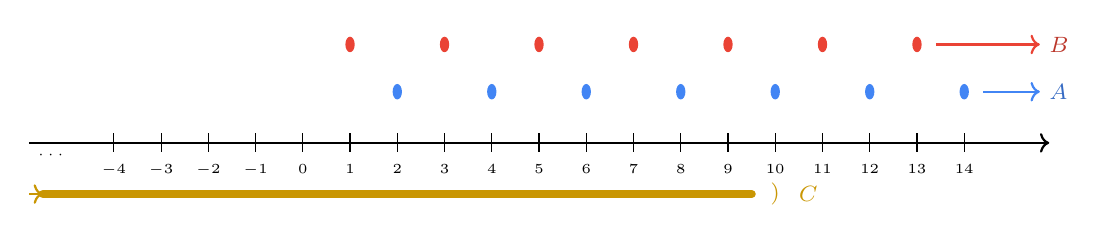
\begin{tikzpicture}[xscale=0.6, font=\small]
  % axis
  \draw[->, thick] (-5.8,0) -- (15.8,0);
  \foreach \x in {-4,-3,...,14} {
    \draw (\x, 0.12) -- (\x, -0.12);
    \node[below, font=\tiny] at (\x, -0.15) {$\x$};
  }
  \node[font=\tiny] at (-5.3, -0.15) {$\cdots$};

  % A: positive evens (blue dots)
  \foreach \x in {2,4,6,8,10,12,14}
    \fill[setA] (\x, 0.65) circle (2.8pt);
  \draw[->, setA, thick] (14.4, 0.65) -- (15.6, 0.65);
  \node[right, setA!80!black, font=\footnotesize] at (15.6, 0.65) {$A$};

  % B: positive odds (red dots)
  \foreach \x in {1,3,5,7,9,11,13}
    \fill[setB] (\x, 1.25) circle (2.8pt);
  \draw[->, setB, thick] (13.4, 1.25) -- (15.6, 1.25);
  \node[right, setB!80!black, font=\footnotesize] at (15.6, 1.25) {$B$};

  % C: x < 10 (yellow bar)
  \draw[setC!80!black, line width=3pt, line cap=round]
    (-5.5, -0.65) -- (9.5, -0.65);
  \draw[<-, setC!80!black, thick] (-5.5, -0.65) -- (-5.8, -0.65);
  \node[setC!80!black, font=\footnotesize] at (10.0, -0.65) {$)$};
  \node[right, setC!80!black, font=\footnotesize] at (10.3, -0.65) {$C$};
\end{tikzpicture}
\end{center}

\textbf{Նախ թարգմանեք յուրաքանչյուր գործողություն բառերով.}
\begin{itemize}[nosep]
  \item $\comp{A}$: ամբողջ թվեր, որոնք դրական զույգ \textbf{չեն}։
  \item $A \symdiff B$: ամբողջ թվեր, որոնք $A, B$-ից \textbf{ճիշտ մեկում} են։
  \item $\comp{C}$: ամբողջ թվեր, որոնք $10$-ից փոքր \textbf{չեն}։
  \item $A \setminus C$: դրական զույգ թվեր, որոնք $C$-ում \textbf{չեն} (այսինքն՝ $\ge 10$)։
  \item $C \setminus (A \symdiff B)$: ամբողջ թվեր $< 10$, որոնք դրական \textbf{չեն}։
\end{itemize}

\medskip
\textbf{(a)\; $\comp{A}$:}\;
Ամեն ինչ $\Z$-ում, որը դրական զույգ ամբողջ թիվ \emph{չէ}։
\[
  \boxed{\comp{A} = \{\ldots, -2, -1, 0\} \;\cup\; \{1, 3, 5, 7, \ldots\}
         = \bigl\{x \in \Z \mid x \le 0 \text{ կամ } x \text{-ը կենտ է}\bigr\}}
\]

\textbf{(b)\; $A \symdiff B$:}\;
Քանի որ $A \cap B = \varnothing$ (ոչ մի ամբողջ թիվ միաժամանակ և՛ դրական զույգ չէ, և՛ դրական կենտ)․
\[
  A \symdiff B = A \cup B = \{1, 2, 3, 4, \ldots\}
\]
Քանի որ յուրաքանչյուր դրական ամբողջ թիվ կա՛մ զույգ է, կա՛մ կենտ (և երբեք միաժամանակ երկուսը լինել չի կարող), ստանում ենք $A \cup B = \Z^+$ և $A \cap B = \varnothing$։
\[
  \boxed{A \symdiff B = \Z^+}
\]

\textbf{(c)\; $\comp{C}$:}\;
Բոլոր ամբողջ թվերը $\ge 10$։
$\quad\boxed{\comp{C} = \{10, 11, 12, \ldots\}}$

\textbf{(d)\; $A \setminus C$:}\;
Դրական զույգ թվեր, որոնք $\ge 10$ են։
$\quad\boxed{A \setminus C = \{10, 12, 14, \ldots\} = \{2k \mid k \ge 5\}}$

\textbf{(e)\; $C \setminus (A \symdiff B)$:}\;
Սա բաղադրյալ գործողություն է։ կատարեք այն քայլ առ քայլ։

\begin{enumerate}[label=\textbf{Քայլ \arabic*։}, leftmargin=*, nosep, itemsep=4pt]
  \item \textbf{Հաշվեք ներքին փակագծերը.}\;
        $A \symdiff B$. Վերևի (b) մասից արդեն գիտենք
        $\boxed{A \symdiff B = \Z^+}$ (բոլոր դրական ամբողջ թվերը)։

  \item \textbf{Տեղադրեք արտաքին գործողության մեջ.}\;
        $C \setminus (A \symdiff B) = C \setminus \Z^+$.
        Սա նշանակում է՝ վերցնել $C$-ի բոլոր տարրերը (ամբողջ թվեր $< 10$) և
        հեռացնել յուրաքանչյուր դրական ամբողջ թիվ։

  \item \textbf{Հաշվեք արդյունքը.}\;
        $C$-ի տարրերը, որոնք դրական \emph{չեն},
        $\ldots, -2, -1, 0$ թվերն են։
\end{enumerate}
\[
  \boxed{C \setminus (A \symdiff B) = \{\ldots, -2, -1, 0\}
         = \{x \in \Z \mid x \le 0\}}
\]

% ══════════════════════════════════════════════════════════════════
\newpage
\section{Խնդիր 20 — $\subseteq$-ի համարժեք բնութագրեր}
% ══════════════════════════════════════════════════════════════════

\begin{theorybox}[Ցիկլային հետևության ապացուցման ռազմավարություն]
Ցույց տալու համար, որ երեք պայմաններ՝ $(a)$, $(b)$, $(c)$, համարժեք են, բավական է ապացուցել
\textbf{հետևությունների ցիկլ}։
\[
  (a) \;\Longrightarrow\; (b) \;\Longrightarrow\; (c) \;\Longrightarrow\; (a):
\]
Սա ավելի արդյունավետ է, քան բոլոր վեց զույգային հետևությունները ուղղակիորեն ապացուցելը։

\begin{center}
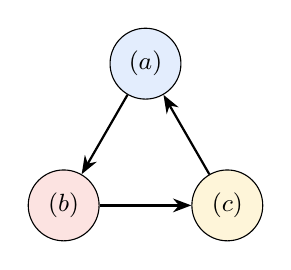
\begin{tikzpicture}[>=Stealth, font=\small]
  \node[draw, circle, minimum size=0.9cm, fill=setA!15] (a) at (90:1.2) {$(a)$};
  \node[draw, circle, minimum size=0.9cm, fill=setB!15] (b) at (210:1.2) {$(b)$};
  \node[draw, circle, minimum size=0.9cm, fill=setC!15] (c) at (330:1.2) {$(c)$};
  \draw[->, thick] (a) -- (b);
  \draw[->, thick] (b) -- (c);
  \draw[->, thick] (c) -- (a);
\end{tikzpicture}
\end{center}
\end{theorybox}

\begin{problembox}
Ապացուցեք, որ $U$ ունիվերսալ բազմության ցանկացած $A, B$ ենթաբազմությունների համար
յուրաքանչյուր խմբի պայմանները համարժեք են․
\begin{enumerate}[nosep]
  \item $A \subseteq B \;\iff\; A \cup B = B \;\iff\; A \cap B = A$
  \item $A \cap B = \varnothing \;\iff\; A \subseteq \comp{B} \;\iff\; B \subseteq \comp{A}$
  \item $A \cup B = U \;\iff\; \comp{A} \subseteq B \;\iff\; \comp{B} \subseteq A$
\end{enumerate}
\end{problembox}

\begin{tcolorbox}[colback=theoryBg, colframe=theoryFrame!80!black, arc=2mm, left=5pt, right=5pt, top=5pt, bottom=5pt, title={\small Տեսողական ինտուիցիա. Ինչո՞ւ են այս պայմանները համարժեք}]
Նախքան ֆորմալ ապացույցին անցնելը, դիտարկեք այս Վենի դիագրամը, որը ցույց է տալիս $A \subseteq B$ (այսինքն՝ $A$-ն ամբողջությամբ գտնվում է $B$-ի ներսում)․

\begin{center}
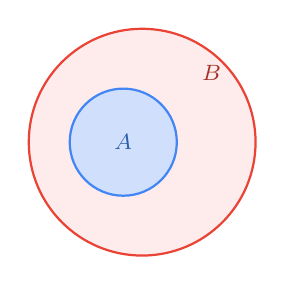
\begin{tikzpicture}[scale=0.8]
  \draw[thick, setB, fill=setB!10] (0,0) circle (1.8);
  \draw[thick, setA, fill=setA!25] (-0.3,0) circle (0.85);
  \node[font=\footnotesize\bfseries, setA!70!black] at (-0.3,0) {$A$};
  \node[font=\footnotesize\bfseries, setB!70!black] at (1.1,1.1) {$B$};
\end{tikzpicture}
\end{center}

\begin{itemize}[nosep]
  \item \textbf{Ինչո՞ւ $A \cup B = B$։} Քանի որ $A$-ն արդեն $B$-ի ներսում է, $A$-ն միավորմանը ավելացնելը ոչինչ չի փոխում։ $A \cup B$-ի ստվերագծված տիրույթը ուղղակի $B$-ն է։
  \item \textbf{Ինչո՞ւ $A \cap B = A$։} $A$-ի յուրաքանչյուր տարր նաև $B$-ում է (քանի որ $A$-ն $B$-ի ներսում է), ուստի $B$-ի հետ հատումը պահպանում է ամբողջ $A$-ն։ $A$-ից ոչինչ չի հեռացվում։
\end{itemize}

Այս պատկերը ստեղծում է տպավորություն, որ բոլոր երեք պայմանները նույն պնդումն են տարբեր բառերով։ Ստորև բերված ֆորմալ ցիկլային հետևության ապացույցը խստորեն հաստատում է դա։
\end{tcolorbox}

% ---- Part 1 ----
\subsection*{Մաս 1.\; $A \subseteq B \;\iff\; A \cup B = B \;\iff\; A \cap B = A$}

\begin{center}
\begin{tikzpicture}[scale=0.72]
  % A subset B
  \draw[thick, setB, fill=setB!10] (0,0) circle (1.6);
  \draw[thick, setA, fill=setA!20] (-0.3,0) circle (0.8);
  \node[font=\footnotesize\bfseries, setA!70!black] at (-0.3,0) {$A$};
  \node[font=\footnotesize\bfseries, setB!70!black] at (0.9,1.0) {$B$};
  \node[font=\footnotesize] at (0, -2.2) {$A \subseteq B$};

  \begin{scope}[xshift=4.5cm]
    \draw[thick, setB, fill=setB!25] (0,0) circle (1.6);
    \draw[thick, setA, dashed] (-0.3,0) circle (0.8);
    \node[font=\footnotesize] at (0, -2.2) {$A \cup B = B$};
    \node[font=\footnotesize, setB!70!black] at (0,0) {ամբողջ $B$-ն};
  \end{scope}

  \begin{scope}[xshift=9cm]
    \draw[thick, setB, dashed] (0,0) circle (1.6);
    \draw[thick, setA, fill=setA!25] (-0.3,0) circle (0.8);
    \node[font=\footnotesize] at (0, -2.2) {$A \cap B = A$};
    \node[font=\footnotesize, setA!70!black] at (-0.3,0) {$A$};
  \end{scope}

  % arrows between diagrams
  \draw[<->, thick, gray] (1.9, 0) -- (2.6, 0);
  \draw[<->, thick, gray] (6.4, 0) -- (7.1, 0);
\end{tikzpicture}
\end{center}

\smallskip
\textit{Հիմնական գաղափար. եթե $A$-ն արդեն $B$-ի ներսում է, $A$-ն միավորմանը ավելացնելը ոչինչ չի փոխում, իսկ $B$-ի հետ հատումը պահպանում է ամբողջ $A$-ն։}

\smallskip
\textbf{$(a) \Rightarrow (b)$։}\;
$A \subseteq B \;\Longrightarrow\; A \cup B = B$.

($\supseteq$)\; $B \subseteq A \cup B$ միշտ։

($\subseteq$)\; Դիցուք $x \in A \cup B$։
Ապա $x \in A$ կամ $x \in B$։
Եթե $x \in A$, ապա $A \subseteq B$-ից հետևում է $x \in B$։
Ցանկացած դեպքում $x \in B$։ \qed

\textbf{$(b) \Rightarrow (c)$։}\;
$A \cup B = B \;\Longrightarrow\; A \cap B = A$.

($\subseteq$)\; $A \cap B \subseteq A$ միշտ։

($\supseteq$)\; Դիցուք $x \in A$։
Ապա $x \in A \cup B = B$, ուստի $x \in B$։
Հետևաբար $x \in A \cap B$։ \qed

\textbf{$(c) \Rightarrow (a)$։}\;
$A \cap B = A \;\Longrightarrow\; A \subseteq B$.

Դիցուք $x \in A$։ Ապա $x \in A = A \cap B$, ուստի $x \in B$։ \qed

% ---- Part 2 ----
\subsection*{Մաս 2.\; $A \cap B = \varnothing \;\iff\; A \subseteq \comp{B} \;\iff\; B \subseteq \comp{A}$}

\begin{center}
\begin{tikzpicture}[scale=0.72]
  \draw[thick, gray] (-2.3,-1.7) rectangle (2.3,1.7);
  \node[gray, font=\scriptsize] at (2.0,1.45) {$U$};
  \draw[thick, setA, fill=setA!20] (-0.85,0) circle (0.9);
  \draw[thick, setB, fill=setB!20] (0.85,0) circle (0.9);
  \node[font=\footnotesize\bfseries, setA!70!black] at (-0.85,0) {$A$};
  \node[font=\footnotesize\bfseries, setB!70!black] at (0.85,0) {$B$};
  \node[font=\footnotesize] at (0,-2.3) {Չհատվող. $A \cap B = \varnothing$};
  \node[font=\scriptsize, gray] at (0, 0) {$\varnothing$};
\end{tikzpicture}
\end{center}

\smallskip
\textit{Հիմնական գաղափար. չհատվող լինելը նշանակում է՝ $A$-ի յուրաքանչյուր տարր գտնվում է $B$-ից դուրս, այսինքն՝ $\comp{B}$-ում։}

\smallskip
\textbf{$(a) \Rightarrow (b)$։}\;
$A \cap B = \varnothing \;\Longrightarrow\; A \subseteq \comp{B}$.

Դիցուք $x \in A$։ Եթե $x \in B$, ապա $x \in A \cap B = \varnothing$, ինչը հակասություն է։
Ուստի $x \notin B$, այսինքն՝ $x \in \comp{B}$։ \qed

\textbf{$(b) \Rightarrow (c)$։}\;
$A \subseteq \comp{B} \;\Longrightarrow\; B \subseteq \comp{A}$.

Դիցուք $x \in B$։ Եթե $x \in A$, ապա $x \in \comp{B}$ (քանի որ $A \subseteq \comp{B}$),
ուստի $x \notin B$, ինչը հակասություն է։ Հետևաբար $x \notin A$, այսինքն՝ $x \in \comp{A}$։ \qed

\textbf{$(c) \Rightarrow (a)$։}\;
$B \subseteq \comp{A} \;\Longrightarrow\; A \cap B = \varnothing$.

Ենթադրենք $x \in A \cap B$։ Ապա $x \in B \subseteq \comp{A}$,
ուստի $x \notin A$, ինչը հակասում է $x \in A \cap B$-ին։ \qed

% ---- Part 3 ----
\subsection*{Մաս 3.\; $A \cup B = U \;\iff\; \comp{A} \subseteq B \;\iff\; \comp{B} \subseteq A$}

\begin{center}
\begin{tikzpicture}[scale=0.72]
  % Shading: entire U is covered
  \draw[thick, gray, fill=gray!8] (-2.3,-1.7) rectangle (2.3,1.7);
  \node[gray, font=\scriptsize] at (2.0,1.45) {$U$};
  \fill[setA!20] (-0.5,0) circle (1.1);
  \fill[setB!20] (0.5,0) circle (1.1);
  % overlap
  \begin{scope}
    \clip (-0.5,0) circle (1.1);
    \fill[purple!15] (0.5,0) circle (1.1);
  \end{scope}
  \draw[thick, setA] (-0.5,0) circle (1.1);
  \draw[thick, setB] (0.5,0) circle (1.1);
  \node[font=\footnotesize\bfseries, setA!70!black] at (-1.1,0) {$A$};
  \node[font=\footnotesize\bfseries, setB!70!black] at (1.1,0) {$B$};
  \node[font=\footnotesize] at (0,-2.3) {Ծածկում. $A \cup B = U$};
\end{tikzpicture}
\end{center}

\smallskip
\textit{Հիմնական գաղափար. եթե $A$-ն և $B$-ն միասին ծածկում են $U$-ն, ապա $A$-ից դուրս ցանկացած բան պետք է լինի $B$-ում։}

\smallskip
\textbf{$(a) \Rightarrow (b)$։}\;
$A \cup B = U \;\Longrightarrow\; \comp{A} \subseteq B$.

Դիցուք $x \in \comp{A}$, այսինքն՝ $x \notin A$։
Քանի որ $x \in U = A \cup B$ և $x \notin A$, ապա պետք է, որ $x \in B$։ \qed

\textbf{$(b) \Rightarrow (c)$։}\;
$\comp{A} \subseteq B \;\Longrightarrow\; \comp{B} \subseteq A$.

Դիցուք $x \in \comp{B}$, այսինքն՝ $x \notin B$։
Եթե $x \notin A$, ապա $x \in \comp{A} \subseteq B$, ինչը տալիս է $x \in B$, որը հակասություն է։
Ուստի $x \in A$։ \qed

\textbf{$(c) \Rightarrow (a)$։}\;
$\comp{B} \subseteq A \;\Longrightarrow\; A \cup B = U$.

Դիցուք $x \in U$։ Կա՛մ $x \in B$ (այդ դեպքում $x \in A \cup B$),
կա՛մ $x \notin B$ (այդ դեպքում $x \in \comp{B} \subseteq A$, ուստի $x \in A \cup B$)։
Քանի որ նաև $A \cup B \subseteq U$, ստանում ենք $A \cup B = U$։ \qed

% ══════════════════════════════════════════════════════════════════
\newpage
\section{Խնդիր 54.3 — $(A \cup B) \setminus C = (A \setminus C) \cup (B \setminus C)$}
% ══════════════════════════════════════════════════════════════════

\begin{theorybox}[Տարբերության բաշխականությունը միավորման նկատմամբ]
Մտավոր մոդել. «$X \setminus C$» նշանակում է
«սկսիր $X$-ից, \textbf{հեռացրու} այն ամենը, ինչ $C$-ում է»։

Միավորումից $C$ բազմությունը հեռացնելը համարժեք է յուրաքանչյուր բազմությունից այն առանձին հեռացնելուն և ստացված մնացորդները միավորելուն։

\begin{center}
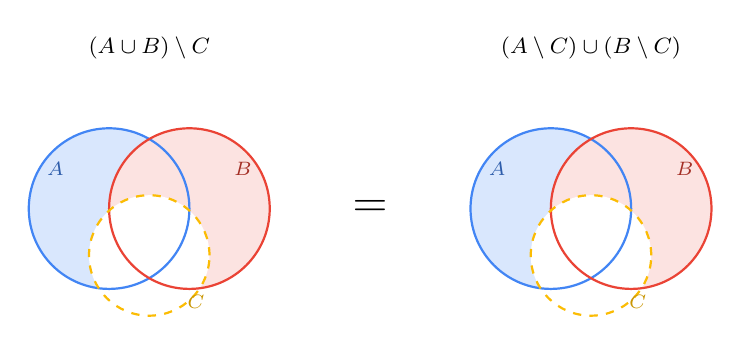
\begin{tikzpicture}[scale=0.85]
  % --- LHS ---
  \begin{scope}[xshift=0cm]
    \node[font=\footnotesize\bfseries] at (0, 2.4) {$(A \cup B) \setminus C$};
    % shade A\C
    \begin{scope}
      \clip (-0.6,0) circle (1.2);
      \fill[setA!20] (-3,-3) rectangle (3,3);
    \end{scope}
    % shade B\C
    \begin{scope}
      \clip (0.6,0) circle (1.2);
      \fill[setB!15] (-3,-3) rectangle (3,3);
    \end{scope}
    % cut out C
    \fill[white] (0, -0.7) circle (0.9);

    \draw[thick, setA] (-0.6, 0) circle (1.2);
    \draw[thick, setB] (0.6, 0) circle (1.2);
    \draw[thick, setC, dashed] (0, -0.7) circle (0.9);
    \node[font=\scriptsize, setA!70!black] at (-1.4, 0.6) {$A$};
    \node[font=\scriptsize, setB!70!black] at (1.4, 0.6) {$B$};
    \node[font=\scriptsize, setC!80!black] at (0.7, -1.4) {$C$};
  \end{scope}

  \node[font=\LARGE] at (3.3, 0) {$=$};

  % --- RHS ---
  \begin{scope}[xshift=6.6cm]
    \node[font=\footnotesize\bfseries] at (0, 2.4) {$(A \setminus C) \cup (B \setminus C)$};
    % shade A\C
    \begin{scope}
      \clip (-0.6,0) circle (1.2);
      \fill[setA!20] (-3,-3) rectangle (3,3);
    \end{scope}
    % shade B\C
    \begin{scope}
      \clip (0.6,0) circle (1.2);
      \fill[setB!15] (-3,-3) rectangle (3,3);
    \end{scope}
    % cut out C
    \fill[white] (0, -0.7) circle (0.9);

    \draw[thick, setA] (-0.6, 0) circle (1.2);
    \draw[thick, setB] (0.6, 0) circle (1.2);
    \draw[thick, setC, dashed] (0, -0.7) circle (0.9);
    \node[font=\scriptsize, setA!70!black] at (-1.4, 0.6) {$A$};
    \node[font=\scriptsize, setB!70!black] at (1.4, 0.6) {$B$};
    \node[font=\scriptsize, setC!80!black] at (0.7, -1.4) {$C$};
  \end{scope}
\end{tikzpicture}
\end{center}
Երկու դիագրամները ստվերագծում են ճիշտ նույն տիրույթը՝ $A$-ի և $B$-ի այն մասերը,
որոնք $C$-ից դուրս են։
\end{theorybox}

\begin{problembox}
Ապացուցեք․\quad $(A \cup B) \setminus C = (A \setminus C) \cup (B \setminus C)$։
\end{problembox}

\subsection*{Լուծում}

Դիցուք $x$-ը կամայական է․
\begin{align*}
  x \in (A \cup B) \setminus C
  &\iff x \in (A \cup B) \;\land\; x \notin C \\
  &\iff (x \in A \;\lor\; x \in B) \;\land\; x \notin C \\
  &\iff (x \in A \land x \notin C)
        \;\lor\; (x \in B \land x \notin C)
        && \text{($\land$-ը բաշխվում է $\lor$-ի նկատմամբ)} \\
  &\iff x \in (A \setminus C) \;\lor\; x \in (B \setminus C) \\
  &\iff x \in (A \setminus C) \cup (B \setminus C):
\end{align*}
Յուրաքանչյուր քայլ $\iff$ է, ուստի բազմությունները հավասար են։ \qed

\smallskip
\textbf{Բազմությունների լեզվով ընթերցում.}\; «$C$-ից դուրս» լինելը «$A$-ում կամ $B$-ում»-ի վրա բաշխելը տրամաբանական $p \land (q \lor r) \iff (p \land q) \lor (p \land r)$ օրենքի բազմությունների տարբերակն է։

\medskip
\begin{tcolorbox}[colback=theoryBg, colframe=theoryFrame!80!black, arc=2mm, left=5pt, right=5pt, top=5pt, bottom=5pt, title={\small Տիրույթների համարակալման մեթոդ — Էմպիրիկ ստուգում}]
\textbf{Տեխնիկա.}\; Երեք բազմությամբ Վենի դիագրամում կան $2^3 = 8$ տիրույթներ։
Համարակալեք դրանք ըստ այն բանի, թե որ բազմություններին են պատկանում․

\begin{center}
\renewcommand{\arraystretch}{1.2}
\begin{tabular}{cl}
\toprule
\textbf{Տիրույթ} & \textbf{Պատկանելիություն} \\
\midrule
1 & միայն $A$ \\
2 & միայն $B$ \\
3 & միայն $C$ \\
4 & միայն $A \cap B$ ($C$-ում չէ) \\
5 & միայն $A \cap C$ ($B$-ում չէ) \\
6 & միայն $B \cap C$ ($A$-ում չէ) \\
7 & $A \cap B \cap C$ \\
8 & Ոչ մեկը ($\comp{A} \cap \comp{B} \cap \comp{C}$) \\
\bottomrule
\end{tabular}
\end{center}

Այժմ արտահայտենք հավասարության յուրաքանչյուր կողմն ըստ իր տիրույթների համարների։
\begin{itemize}[nosep]
  \item $A \cup B = \{1, 2, 4, 5, 6, 7\}$
  \item $(A \cup B) \setminus C$: հեռացնել $C$-ի տիրույթները ($\{3,5,6,7\}$)
        $\;\Longrightarrow\; \boxed{\{1, 2, 4\}}$
  \item $A \setminus C = \{1, 4\}$, \quad $B \setminus C = \{2, 4\}$
  \item $(A \setminus C) \cup (B \setminus C) = \{1, 4\} \cup \{2, 4\} = \boxed{\{1, 2, 4\}}$
\end{itemize}

Երկու կողմերն էլ տալիս են ճիշտ նույն տիրույթները $\{1, 2, 4\}$, ինչը էմպիրիկորեն հաստատում է նույնությունը։

\medskip
\textit{Այս մեթոդը չի փոխարինում ապացույցին, բայց հիանալի միջոց է վստահություն ձեռք բերելու կամ սխալները հայտնաբերելու համար նախքան ապացույցը գրելը։}
\end{tcolorbox}

\end{document}
\newpage

% ── Practice 2-3 ─────────────────────────────────────────────────
\section{Գործնական 2-3 — Հարաբերություններ}
\documentclass[12pt, a4paper]{article}

% ── Packages ──────────────────────────────────────────────────────
\usepackage{fontspec}
\setmainfont{Arial}
\usepackage{amsmath, amssymb, amsthm}
\usepackage{mathtools}
\usepackage{enumitem}
\usepackage{tikz}
\usetikzlibrary{calc, positioning, arrows.meta, fit, patterns, decorations.pathreplacing, shapes.geometric}
\usepackage{geometry}
\geometry{margin=2.4cm}
\usepackage{xcolor}
\usepackage{tcolorbox}
\tcbuselibrary{theorems, skins, breakable}
\usepackage{booktabs}
\usepackage{colortbl}
\usepackage{hyperref}
\hypersetup{colorlinks=true, linkcolor=blue!60!black, urlcolor=blue!60!black}

\setlength{\parindent}{0pt}
\setlength{\parskip}{6pt}

% ── Colours ───────────────────────────────────────────────────────
\definecolor{setA}{RGB}{66, 133, 244}   % blue
\definecolor{setB}{RGB}{234, 67, 53}    % red
\definecolor{setC}{RGB}{251, 188, 4}    % yellow
\definecolor{newEdge}{RGB}{39, 174, 96} % green for added edges
\definecolor{diagGray}{gray}{0.85}      % matrix diagonal shading
\definecolor{mirrorBlue}{RGB}{173,216,230}  % mirrored pair highlight (light blue)
\definecolor{mirrorRose}{RGB}{255,204,204}  % mirrored pair highlight (light rose)
\definecolor{theoryBg}{RGB}{232, 245, 253}
\definecolor{theoryFrame}{RGB}{66, 133, 244}
\definecolor{stmtBg}{RGB}{255, 243, 224}
\definecolor{stmtFrame}{RGB}{230, 126, 34}
\definecolor{ansBg}{RGB}{232, 250, 232}
\definecolor{ansFrame}{RGB}{39, 174, 96}

% ── Environments ──────────────────────────────────────────────────
\newtcolorbox{theorybox}[1][]{%
  colback=theoryBg, colframe=theoryFrame,
  fonttitle=\bfseries, title={\small Տեսության ամփոփում. #1},
  breakable, enhanced, arc=2mm,
  left=5pt, right=5pt, top=5pt, bottom=5pt
}

\newtcolorbox{problembox}{%
  colback=stmtBg, colframe=stmtFrame,
  fonttitle=\bfseries, title={\small Խնդրի դրվածք},
  breakable, enhanced, arc=2mm,
  left=5pt, right=5pt, top=5pt, bottom=5pt
}

\newtcolorbox{answerbox}{%
  colback=ansBg, colframe=ansFrame,
  arc=2mm, left=5pt, right=5pt, top=3pt, bottom=3pt
}

\newcommand{\Z}{\mathbb{Z}}
\newcommand{\R}{\mathbb{R}}
\newcommand{\N}{\mathbb{N}}
\newcommand{\Q}{\mathbb{Q}}

% ── Title ─────────────────────────────────────────────────────────
\title{\textbf{Գործնական 2--3 — Հարաբերություններ}\\[4pt]
       \large Ընտրված խնդիրների լուծումներ\\[2pt]
       \normalsize Խնդիրներ 1.2,\; 2.1,\; 2.2,\; 3.3,\; 4.1,\; 7.2}
\author{Դիսկրետ մաթեմատիկա — ԵՊՀ}
\date{}

\begin{document}
\maketitle
\tableofcontents
\newpage

% ══════════════════════════════════════════════════════════════════
\section{Խնդիր 1.2 — Հարաբերությունների որոշման և արժեքների տիրույթներ}
% ══════════════════════════════════════════════════════════════════

\begin{theorybox}[Որոշման և Արժեքների տիրույթներ]
$\alpha \subseteq A \times B$ հարաբերության համար։
\begin{itemize}[nosep]
  \item \textbf{Որոշման տիրույթ՝} $D_\alpha = \{\,x \mid \exists\, y:\; (x,y) \in \alpha\,\}$ — բոլոր առաջին կոորդինատների բազմությունը։
  \item \textbf{Արժեքների տիրույթ՝} $R_\alpha = \{\,y \mid \exists\, x:\; (x,y) \in \alpha\,\}$ — բոլոր երկրորդ կոորդինատների բազմությունը։
\end{itemize}
\end{theorybox}

\begin{problembox}
Գտեք $D_\alpha$ որոշման տիրույթը և $R_\alpha$ արժեքների տիրույթը հետևյալ հարաբերություններից յուրաքանչյուրի համար։
\end{problembox}

\textbf{Մեթոդ.}\; Որոշման տիրույթը գտնելու համար ֆիքսեք $x$-ը և **ստուգեք՝** արդյոք գոյություն ունի \textbf{որևէ} $y$, որը բավարարում է հարաբերությանը։ Արժեքների տիրույթը գտնելու համար ֆիքսեք $y$-ը և **ստուգեք՝** արդյոք գոյություն ունի \textbf{որևէ} $x$։

\medskip

\begin{tcolorbox}[colback=blue!3, colframe=setA!60, arc=2mm, left=5pt, right=5pt, top=4pt, bottom=4pt,
  fonttitle=\bfseries, title={\small Ինտուիցիա. Ստվերի պրոյեկցիայի անալոգիա}]
Պատկերացրեք $\alpha \subseteq \R^2$ հարաբերությունը որպես $xy$-հարթության վրա գծված \textbf{երկչափ (2D) պատկեր}։
\begin{itemize}[nosep]
  \item \textbf{Որոշման տիրույթը}՝ $D_\alpha$-ն, այն \emph{ստվերն} է, որը պատկերը գցում է $x$-առանցքի վրա
        (լույսն ուղղեք վերևից ներքև և ստուգեք, թե $x$-ի որ արժեքներն են «լուսավորվում»)։
  \item \textbf{Արժեքների տիրույթը}՝ $R_\alpha$-ն, այն ստվերն է, որը գցվում է $y$-առանցքի վրա
        (լույսը ուղղեք աջից և տեսեք, թե որ $y$-արժեքներն են «լուսավորվում»)։
\end{itemize}
\smallskip
Օրինակ՝ $x^2 + y^2 \le 16$ շրջանը 4 շառավղով լցված շրջան է։
Դրա ստվերը յուրաքանչյուր առանցքի վրա $[-4,\,4]$ միջակայքն է, ուստի $D_\alpha$ և $R_\alpha$ հավասար են $[-4,\,4]$։

Այս «ստվերի» պատկերացումը աշխատում է անհավասարությամբ կամ հավասարումով տրված \emph{ցանկացած} երկրաչափական հարաբերության համար։
\end{tcolorbox}

\medskip

%────────────────────────────────────────
\subsection*{(a)\; $\alpha = \{(a,1),\,(a,2),\,(c,1),\,(c,2),\,(c,4),\,(d,5)\}$}

Կարդալով առաջին և երկրորդ կոորդինատները՝

\begin{answerbox}
$D_\alpha = \{a,\, c,\, d\}, \qquad R_\alpha = \{1,\, 2,\, 4,\, 5\}։$
\end{answerbox}

%────────────────────────────────────────
\subsection*{(b)\; $\alpha = \{(1,2),\,(2,4),\,(3,6),\,(4,8),\,\dots\}$}

Օրինաչափությունը $(n,\,2n)$ է $n \in \N$-ի համար, ուստի։

\begin{answerbox}
$D_\alpha = \N = \{1,2,3,\dots\}, \qquad
  R_\alpha = \{2,4,6,8,\dots\} = 2\N։$
\end{answerbox}

%────────────────────────────────────────
\subsection*{(c)\; $\alpha = \{(x,y) \in \R^2 \mid x = y^2\}$}

Քանի որ $x = y^2 \ge 0$ բոլոր $y$-ների համար, և յուրաքանչյուր $x \ge 0$-ի համար գոյություն ունի $y = \pm\sqrt{x}$։
Քառակուսիները երբեք բացասական չեն լինում, ուստի $x$-ի բացասական արժեքները որոշման տիրույթում չեն կարող լինել։

\begin{answerbox}
$D_\alpha = [0, +\infty), \qquad R_\alpha = \R։$
\end{answerbox}

\begin{center}
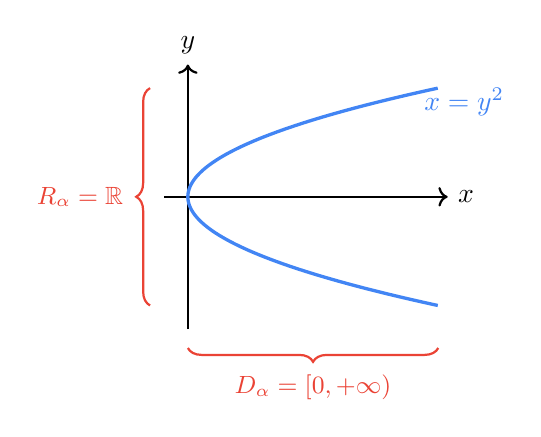
\begin{tikzpicture}[scale=0.6]
  \draw[->, thick] (-0.5,0) -- (5.5,0) node[right] {$x$};
  \draw[->, thick] (0,-2.8) -- (0,2.8) node[above] {$y$};
  \draw[setA, very thick, domain=-2.3:2.3, samples=100] plot ({(\x)^2}, \x);
  \node[setA, right] at (4.8, 2) {$x = y^2$};
  % Braces for D and R
  \draw[thick, setB, decorate, decoration={brace, amplitude=5pt, mirror}]
    (0,-3.2) -- (5.3,-3.2) node[midway, below=6pt, setB] {\small $D_\alpha = [0,+\infty)$};
  \draw[thick, setB, decorate, decoration={brace, amplitude=5pt}]
    (-0.8,-2.3) -- (-0.8,2.3) node[midway, left=6pt, setB] {\small $R_\alpha = \R$};
\end{tikzpicture}
\end{center}

%────────────────────────────────────────
\subsection*{(d)\; $\alpha = \{(x,y) \in \R^2 \mid x^2 + y^2 \le 16\}$}

Սա 4 շառավղով փակ շրջան է՝ կենտրոնացած կոորդինատների սկզբնակետում։
Ցանկացած $x$-ի համար, որտեղ $|x| \le 4$, գոյություն ունի $y$, որը բավարարում է $x^2 + y^2 \le 16$, և հակառակը։

\begin{answerbox}
$D_\alpha = [-4,\, 4], \qquad R_\alpha = [-4,\, 4]։$
\end{answerbox}

\begin{center}
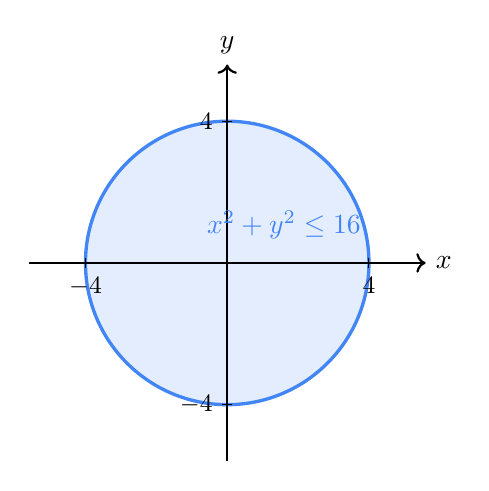
\begin{tikzpicture}[scale=0.6]
  \fill[setA!15] (0,0) circle (3);
  \draw[setA, very thick] (0,0) circle (3);
  \draw[->, thick] (-4.2,0) -- (4.2,0) node[right] {$x$};
  \draw[->, thick] (0,-4.2) -- (0,4.2) node[above] {$y$};
  \foreach \v/\lab in {-3/{-4}, 3/4} {
    \draw (\v, 0.1) -- (\v, -0.1) node[below]{\small $\lab$};
    \draw (0.1, \v) -- (-0.1, \v) node[left]{\small $\lab$};
  }
  \node[setA] at (1.2, 0.8) {$x^2+y^2 \le 16$};
\end{tikzpicture}
\end{center}

%────────────────────────────────────────
\subsection*{(e)\; $\alpha = \{(x,y) \in \N^2 \mid x \le y\}$}

Յուրաքանչյուր $x \in \N$ հարաբերվում է առնվազն $y=x$-ի հետ, ուստի $D_\alpha = \N$։
Յուրաքանչյուր $y \in \N$ հանդես է գալիս որպես երկրորդ կոորդինատ (վերցրեք $x=y$), ուստի $R_\alpha = \N$։

\begin{answerbox}
$D_\alpha = \N, \quad R_\alpha = \N։$
\end{answerbox}

%────────────────────────────────────────
\subsection*{(f)\; $\alpha = \{(x,y) \in \N^2 \mid y \le x\}$}

Նմանապես՝ յուրաքանչյուր $x \in \N$ հարաբերվում է $y=x$-ի հետ, ուստի $D_\alpha = \N$։
Եվ յուրաքանչյուր $y \in \N$-ի համապատասխանում է $x=y$, ուստի $R_\alpha = \N$։

\begin{answerbox}
$D_\alpha = \N, \quad R_\alpha = \N։$
\end{answerbox}

%────────────────────────────────────────
\subsection*{(g)\; $\alpha = \{(x,y) \in \R^2 \mid x + y \ge 0\}$}

Սա $y = -x$ ուղղից վերև և դրա վրա գտնվող կիսահարթությունն է։
Ցանկացած $x \in \R$-ի համար ընտրեք $y = -x + 1$, այդ դեպքում $x + y = 1 \ge 0$։
Ցանկացած $y \in \R$-ի համար ընտրեք $x = -y + 1$։

\begin{answerbox}
$D_\alpha = \R, \quad R_\alpha = \R։$
\end{answerbox}

\begin{center}
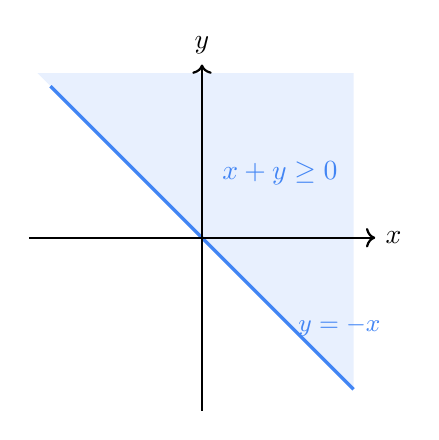
\begin{tikzpicture}[scale=0.55]
  % Shaded half-plane
  \fill[setA!12] (-3.5,3.5) -- (3.5,-3.5) -- (3.5,3.8) -- (-3.8,3.8) -- (-3.5,3.5);
  % Boundary line
  \draw[setA, very thick] (-3.5,3.5) -- (3.5,-3.5);
  % Axes
  \draw[->, thick] (-4,0) -- (4,0) node[right] {$x$};
  \draw[->, thick] (0,-4) -- (0,4) node[above] {$y$};
  \node[setA] at (1.8, 1.5) {$x+y \ge 0$};
  \node[setA, above right] at (2, -2.5) {\small $y=-x$};
\end{tikzpicture}
\end{center}

%────────────────────────────────────────
\subsection*{(h)\; $\alpha = \{(x,y) \in \R^2 \mid 2x \ge 3y\}$}

Համարժեք է $y \le \tfrac{2}{3}\,x$-ին։
Ցանկացած $x$-ի համար ընտրեք $y = 0$ (երբ $x \ge 0$) կամ ցանկացած բավականաչափ փոքր $y$։
Ցանկացած $y$-ի համար ընտրեք $x = \tfrac{3}{2}y$։

\begin{answerbox}
$D_\alpha = \R, \quad R_\alpha = \R։$
\end{answerbox}

% ══════════════════════════════════════════════════════════════════
\newpage
\section{Խնդիր 2.1 — Հարաբերությունների գրաֆ և մատրից}
% ══════════════════════════════════════════════════════════════════

\begin{theorybox}[Հարաբերությունների գրաֆներ և մատրիցներ]
Դիցուք $\alpha$-ն $A = \{a_1,\dots,a_n\}$ վերջավոր բազմության վրա հարաբերություն է։
\begin{itemize}[nosep]
  \item \textbf{Գրաֆ.} $A$-ի յուրաքանչյուր տարր գագաթ է։ Սիմետրիկ հարաբերության համար, եթե $(a_i, a_j) \in \alpha$ և $i \ne j$, տարեք \emph{չուղղորդված} կող $a_i$-ի և $a_j$-ի միջև։
  \item \textbf{Մատրից.} $n \times n$ մատրից $M$, որտեղ $M_{ij} = 1$, եթե $(a_i, a_j) \in \alpha$, և $M_{ij} = 0$ հակառակ դեպքում։ Սիմետրիկ հարաբերության համար $M = M^T$։
\end{itemize}
\end{theorybox}

\begin{problembox}
Կառուցեք գրաֆը և մատրիցը $A = \{a, b, c, d, e\}$ բազմության վրա տրված հետևյալ հարաբերությունների համար։
\end{problembox}

% TikZ style for undirected graph nodes
\tikzset{
  gnode/.style={circle, draw, thick, minimum size=8mm, inner sep=0pt, font=\small},
}

%────────────────────────────────────────
\subsection*{(a)\; $\alpha = \{(a,b),(b,a),(b,c),(c,b),(c,a),(a,c),(d,e),(e,d)\}$}

Քանի որ յուրաքանչյուր զույգ հանդիպում է իր հակառակի հետ, հարաբերությունը սիմետրիկ է։ Չուղղորդված կողեր.
\[
  \boxed{a\text{--}b,\quad b\text{--}c,\quad a\text{--}c,\quad d\text{--}e։}
\]

\begin{center}
\begin{minipage}{0.45\textwidth}\centering
\begin{tikzpicture}
  % Pentagon layout
  \node[gnode] (a) at (90:1.8)  {$a$};
  \node[gnode] (b) at (18:1.8)  {$b$};
  \node[gnode] (c) at (306:1.8) {$c$};
  \node[gnode] (d) at (234:1.8) {$d$};
  \node[gnode] (e) at (162:1.8) {$e$};

  \draw[thick, setA] (a) -- (b);
  \draw[thick, setA] (b) -- (c);
  \draw[thick, setA] (a) -- (c);
  \draw[thick, setA] (d) -- (e);
\end{tikzpicture}
\end{minipage}%
\begin{minipage}{0.5\textwidth}\centering
\textbf{Գունավորված մատրից} (սիմետրիան տեսանելի է)։\\[4pt]
{\small Անկյունագիծ = \colorbox{diagGray}{մոխրագույն},\;
հայելային 1-եր = \colorbox{mirrorBlue}{կապույտ} / \colorbox{mirrorRose}{վարդագույն}։}\\[4pt]
\renewcommand{\arraystretch}{1.15}
$M_\alpha = \left(\;\begin{tabular}{c|ccccc}
  & $a$ & $b$ & $c$ & $d$ & $e$ \\\hline
$a$ & \cellcolor{diagGray}0 & \cellcolor{mirrorBlue}1 & \cellcolor{mirrorRose}1 & 0 & 0 \\
$b$ & \cellcolor{mirrorBlue}1 & \cellcolor{diagGray}0 & \cellcolor{mirrorBlue}1 & 0 & 0 \\
$c$ & \cellcolor{mirrorRose}1 & \cellcolor{mirrorBlue}1 & \cellcolor{diagGray}0 & 0 & 0 \\
$d$ & 0 & 0 & 0 & \cellcolor{diagGray}0 & \cellcolor{mirrorRose}1 \\
$e$ & 0 & 0 & 0 & \cellcolor{mirrorRose}1 & \cellcolor{diagGray}0
\end{tabular}\;\right)$
\end{minipage}
\end{center}

Մատրիցը սիմետրիկ է ($M = M^T$). անկյունագծից վերև գտնվող յուրաքանչյուր ստվերագծված 1-ին համապատասխանում է ներքևում գտնվող ստվերագծված 1։
Երկու կապակցված բաղադրիչներ։ եռանկյունի $\{a,b,c\}$ և կող $\{d,e\}$։

\textbf{Կառուցման կարգ.}\; $A$-ի վրա վերջավոր հարաբերության համար. (1) թվարկեք կարգավորված զույգերը, (2) լրացրեք մատրիցը տող առ տող զույգերից, (3) կարդացեք ուղղորդված գրաֆը մատրիցից։

%────────────────────────────────────────
\subsection*{(b)\; $\alpha = \{(a,b),(b,a),(b,c),(c,b),(c,d),(d,c),(c,a),(a,c)\}$}

Չուղղորդված կողեր.
\[
  \boxed{a\text{--}b,\quad b\text{--}c,\quad c\text{--}d,\quad a\text{--}c։}
\]

\begin{center}
\begin{minipage}{0.45\textwidth}\centering
\begin{tikzpicture}
  \node[gnode] (a) at (90:1.8)  {$a$};
  \node[gnode] (b) at (18:1.8)  {$b$};
  \node[gnode] (c) at (306:1.8) {$c$};
  \node[gnode] (d) at (234:1.8) {$d$};
  \node[gnode] (e) at (162:1.8) {$e$};

  \draw[thick, setA] (a) -- (b);
  \draw[thick, setA] (b) -- (c);
  \draw[thick, setA] (a) -- (c);
  \draw[thick, setA] (c) -- (d);
\end{tikzpicture}
\end{minipage}%
\begin{minipage}{0.5\textwidth}\centering
\renewcommand{\arraystretch}{1.15}
$M_\alpha = \left(\;\begin{tabular}{c|ccccc}
  & $a$ & $b$ & $c$ & $d$ & $e$ \\\hline
$a$ & \cellcolor{diagGray}0 & \cellcolor{mirrorBlue}1 & \cellcolor{mirrorRose}1 & 0 & 0 \\
$b$ & \cellcolor{mirrorBlue}1 & \cellcolor{diagGray}0 & \cellcolor{mirrorBlue}1 & 0 & 0 \\
$c$ & \cellcolor{mirrorRose}1 & \cellcolor{mirrorBlue}1 & \cellcolor{diagGray}0 & \cellcolor{mirrorRose}1 & 0 \\
$d$ & 0 & 0 & \cellcolor{mirrorRose}1 & \cellcolor{diagGray}0 & 0 \\
$e$ & 0 & 0 & 0 & 0 & \cellcolor{diagGray}0
\end{tabular}\;\right)$
\end{minipage}
\end{center}

Եռանկյունի $\{a,b,c\}$, որին կցված է $d$-ն $c$-ի միջոցով; $e$ գագաթը մեկուսացված է։

%────────────────────────────────────────
\subsection*{(c)}

(c) մասը նույնական է (b) մասին սկզբնական խնդրագրքում։ Գրաֆը և մատրիցը նույնն են, ինչ վերևում։

% ══════════════════════════════════════════════════════════════════
\newpage
\section{Խնդիր 2.2 — Հարաբերությունների դիգրաֆ և մատրից}
% ══════════════════════════════════════════════════════════════════

\begin{theorybox}[Ուղղորդված գրաֆներ (Դիգրաֆներ)]
$A$-ի վրա (ոչ անպայման սիմետրիկ) $\alpha$ հարաբերության համար։
\begin{itemize}[nosep]
  \item \textbf{Դիգրաֆ.} Գագաթները $A$-ի տարրերն են։ Յուրաքանչյուր $(a_i,a_j) \in \alpha$-ի համար տարեք սլաք $a_i \to a_j$։ $(a_i,a_i)$ զույգը \emph{օղակ} է։
  \item \textbf{Մատրից.} Նույն կառուցումը; մատրիցը պարտադիր չէ, որ լինի սիմետրիկ։
\end{itemize}
\end{theorybox}

\begin{tcolorbox}[colback=white, colframe=gray!50, arc=2mm, width=0.9\textwidth, halign=center]
  \textbf{Տեսանյութ.} Կառուցել հարաբերության դիգրաֆը և մատրիցը \\
  \href{https://youtu.be/jVi59i_XRBw}{\textbf{[VIDEO]} Դիտել YouTube-ում (ID: jVi59i\_XRBw)}
\end{tcolorbox}

\begin{problembox}
Կառուցեք դիգրաֆը և մատրիցը $A = \{a, b, c, d, e, f\}$ բազմության վրա հետևյալ հարաբերությունների համար։
\end{problembox}

% TikZ style for digraph
\tikzset{
  dnode/.style={circle, draw, thick, minimum size=8mm, inner sep=0pt, font=\small},
  darr/.style={-{Stealth[length=5pt]}, thick, setA},
}

%────────────────────────────────────────
\subsection*{(a)\; $\alpha = \{(a,b),(b,c),(a,c),(b,e),(c,f),(c,d),(d,f),(f,e)\}$}

\begin{center}
\begin{tikzpicture}
  % Layout: top-flow for a→b→c, bottom for e,f,d
  \node[dnode] (a) at (0,2.5)   {$a$};
  \node[dnode] (b) at (2.5,2.5) {$b$};
  \node[dnode] (c) at (5,2.5)   {$c$};
  \node[dnode] (f) at (2.5,0)   {$f$};
  \node[dnode] (e) at (0,0)     {$e$};
  \node[dnode] (d) at (5,0)     {$d$};

  \draw[darr] (a) -- (b);
  \draw[darr] (b) -- (c);
  \draw[darr] (a) edge[bend right=15] (c);
  \draw[darr] (b) edge[bend left=8] (e);
  \draw[darr] (c) -- (f);
  \draw[darr] (c) -- (d);
  \draw[darr] (d) -- (f);
  \draw[darr] (f) -- (e);
\end{tikzpicture}
\end{center}

\[
M_\alpha = \bordermatrix{
  & a & b & c & d & e & f \cr
a & 0 & 1 & 1 & 0 & 0 & 0 \cr
b & 0 & 0 & 1 & 0 & 1 & 0 \cr
c & 0 & 0 & 0 & 1 & 0 & 1 \cr
d & 0 & 0 & 0 & 0 & 0 & 1 \cr
e & 0 & 0 & 0 & 0 & 0 & 0 \cr
f & 0 & 0 & 0 & 0 & 1 & 0 \cr
}
\]

%────────────────────────────────────────
\subsection*{(b)\; $\alpha = \{(a,b),(b,c),(d,c),(d,e),(f,e),(f,a),(b,e)\}$}

\begin{center}
\begin{tikzpicture}
  \node[dnode] (a) at (0,2.5)   {$a$};
  \node[dnode] (b) at (2.5,2.5) {$b$};
  \node[dnode] (c) at (5,2.5)   {$c$};
  \node[dnode] (d) at (5,0)     {$d$};
  \node[dnode] (e) at (2.5,0)   {$e$};
  \node[dnode] (f) at (0,0)     {$f$};

  \draw[darr] (a) -- (b);
  \draw[darr] (b) -- (c);
  \draw[darr] (b) -- (e);
  \draw[darr] (d) -- (c);
  \draw[darr] (d) -- (e);
  \draw[darr] (f) -- (e);
  \draw[darr] (f) -- (a);
\end{tikzpicture}
\end{center}

\[
M_\alpha = \bordermatrix{
  & a & b & c & d & e & f \cr
a & 0 & 1 & 0 & 0 & 0 & 0 \cr
b & 0 & 0 & 1 & 0 & 1 & 0 \cr
c & 0 & 0 & 0 & 0 & 0 & 0 \cr
d & 0 & 0 & 1 & 0 & 1 & 0 \cr
e & 0 & 0 & 0 & 0 & 0 & 0 \cr
f & 1 & 0 & 0 & 0 & 1 & 0 \cr
}
\]

%────────────────────────────────────────
\subsection*{(c)\; $\alpha = \{(a,c),(c,c),(c,d),(c,e),(e,c),(e,e),(e,f),(a,e)\}$}

\begin{center}
\begin{tikzpicture}
  % Reposition: b is isolated, push it aside; cluster active vertices
  \node[dnode] (a) at (0,2)     {$a$};
  \node[dnode] (c) at (3,2)     {$c$};
  \node[dnode] (d) at (5.5,2)   {$d$};
  \node[dnode] (e) at (3,0)     {$e$};
  \node[dnode] (f) at (5.5,0)   {$f$};
  \node[dnode, dashed, gray] (b) at (0,0) {$b$};

  \draw[darr] (a) -- (c);
  \draw[darr] (a) -- (e);
  \draw[darr] (c) edge[loop above, looseness=8, min distance=10mm] (c);
  \draw[darr] (c) -- (d);
  \draw[darr] (c) edge[bend left=12] (e);
  \draw[darr] (e) edge[bend left=12] (c);
  \draw[darr] (e) edge[loop below, looseness=8, min distance=10mm] (e);
  \draw[darr] (e) -- (f);
\end{tikzpicture}
\end{center}

Նշում. $b$ գագաթը (կետագծերով) ամբողջովին մեկուսացված է՝ նրան կողեր չեն դիպչում։

\[
M_\alpha = \bordermatrix{
  & a & b & c & d & e & f \cr
a & 0 & 0 & 1 & 0 & 1 & 0 \cr
b & 0 & 0 & 0 & 0 & 0 & 0 \cr
c & 0 & 0 & 1 & 1 & 1 & 0 \cr
d & 0 & 0 & 0 & 0 & 0 & 0 \cr
e & 0 & 0 & 1 & 0 & 1 & 1 \cr
f & 0 & 0 & 0 & 0 & 0 & 0 \cr
}
\]

$c$-ի և $e$-ի օղակները երևում են որպես 1-եր գլխավոր անկյունագծի վրա։ $b$-ի տողը և $b$-ի սյունակը ամբողջությամբ զրոներ են։

Մատրիցում զրոյական տողը նշանակում է «ելնող կողեր չկան» այդ տարրից։ Զրոյական սյունակը նշանակում է «մտնող կողեր չկան» դեպի այդ տարրը։

%────────────────────────────────────────
\subsection*{Հակադրություն. Սիմետրիկ (2.1) ընդդեմ Ոչ սիմետրիկ (2.2) Մատրիցներ}

Խնդիրներ 2.1-ի և 2.2-ի մատրիցները ցույց են տալիս սիմետրիկ (չուղղորդված) և ընդհանուր (ուղղորդված) հարաբերությունների կառուցվածքային տարբերությունը։ Ստորև մենք տեղադրում ենք 2.1(a)-ի մատրիցը 2.2(a)-ի մատրիցի կողքին։

\begin{center}
\begin{minipage}{0.45\textwidth}\centering
\textbf{Խնդիր 2.1\,(a) — Սիմետրիկ}\\[4pt]
\renewcommand{\arraystretch}{1.15}
$\left(\;\begin{tabular}{ccccc}
0 & 1 & 1 & 0 & 0 \\
1 & 0 & 1 & 0 & 0 \\
1 & 1 & 0 & 0 & 0 \\
0 & 0 & 0 & 0 & 1 \\
0 & 0 & 0 & 1 & 0
\end{tabular}\;\right)$\\[4pt]
{\small $M = M^T$: $(i,j)$ տարրը միշտ հավասար է $(j,i)$ տարրին։\\
Չուղղորդված կողեր; սլաքներ պետք չեն։}
\end{minipage}%
\hfill
\begin{minipage}{0.45\textwidth}\centering
\textbf{Խնդիր 2.2\,(a) — Ոչ սիմետրիկ}\\[4pt]
\renewcommand{\arraystretch}{1.15}
$\left(\;\begin{tabular}{cccccc}
0 & 1 & 1 & 0 & 0 & 0 \\
0 & 0 & 1 & 0 & 1 & 0 \\
0 & 0 & 0 & 1 & 0 & 1 \\
0 & 0 & 0 & 0 & 0 & 1 \\
0 & 0 & 0 & 0 & 0 & 0 \\
0 & 0 & 0 & 0 & 1 & 0
\end{tabular}\;\right)$\\[4pt]
{\small $M \ne M^T$: օր.՝ $M_{12}=1$ բայց $M_{21}=0$.\\
Պահանջվում են ուղղորդված կողեր (սլաքներ)։}
\end{minipage}
\end{center}

%────────────────────────────────────────
\subsection*{Աստիճանի հետևում — Խնդիր 2.2\,(a)}

Ուղղորդված հարաբերության համար յուրաքանչյուր գագաթ ունի \textbf{մուտքային աստիճան} (մտնող կողերի քանակը) և \textbf{ելքային աստիճան} (ելնող կողերի քանակը)։ Դրանք կարդացվում են անմիջապես մատրիցից։ $v$-ի ելքային աստիճանը տողի գումարն է, իսկ մուտքային աստիճանը՝ սյունակի գումարը։

\begin{center}
\renewcommand{\arraystretch}{1.2}
\begin{tabular}{c|c|c}
  \toprule
  \textbf{Գագաթ} & \textbf{Մուտքային աստիճան} & \textbf{Ելքային աստիճան} \\
  \midrule
  $a$ & 0 & 2 \\
  $b$ & 1 & 2 \\
  $c$ & 2 & 2 \\
  $d$ & 1 & 1 \\
  $e$ & 2 & 0 \\
  $f$ & 2 & 1 \\
  \bottomrule
\end{tabular}
\end{center}

Նկատեք, որ $\sum \text{մուտքային աստիճաններ} = \sum \text{ելքային աստիճաններ} = |\alpha| = 8$ (յուրաքանչյուր կող յուրաքանչյուր գումարին ավելացնում է 1)։

$e$ գագաթն ունի 0 ելքային աստիճան, ինչը նրան դարձնում է \emph{կլանիչ} (ելնող սլաքներ չկան)։
$a$ գագաթն ունի 0 մուտքային աստիճան, ինչը նրան դարձնում է \emph{աղբյուր} (մտնող սլաքներ չկան)։

% ══════════════════════════════════════════════════════════════════
\newpage
\section{Խնդիր 3.3 — Հարաբերությունների կոմպոզիցիա}
% ══════════════════════════════════════════════════════════════════

\begin{theorybox}[Հարաբերությունների կոմպոզիցիա]
Դիցուք $\alpha \subseteq A \times B$ և $\beta \subseteq B \times C$։ $\alpha \circ \beta$ \textbf{կոմպոզիցիան} (նաև գրվում է $\alpha \cdot \beta$) հարաբերություն է $A \times C$-ի վրա, որը սահմանվում է։
\[
  (x, z) \in \alpha \circ \beta
  \;\;\Longleftrightarrow\;\;
  \exists\, y \in B:\;
  (x, y) \in \alpha \;\land\; (y, z) \in \beta:
\]
Կարդացեք ձախից աջ։ նախ անցեք $\alpha$-ով ($x$-ից որևէ $y$), այնուհետև $\beta$-ով ($y$-ից $z$)։
\end{theorybox}

\begin{problembox}
Դիցուք $\alpha$ և $\beta$ հարաբերություններ են $\Z$-ի վրա։
\[
  \alpha = \{(x,\, x+2) \mid x \in \Z\}, \qquad
  \beta  = \{(x,\, x-2) \mid x \in \Z\}:
\]
Գտեք $\alpha \circ \beta$ և $\beta \circ \alpha$։
\end{problembox}

\textbf{Պայմանավորվածություն.}\; Հարաբերությունների կոմպոզիցիան այստեղ կարդացվում է \textbf{ձախից աջ}։ $\alpha \circ \beta$-ում նախ կիրառեք $\alpha$-ն, հետո $\beta$-ն։ Սա սխալների ամենատարածված աղբյուրն է։

\medskip

\subsection*{$\alpha \circ \beta$-ի որոշումը}

Նախ կիրառում ենք $\alpha$-ն, ապա՝ $\beta$-ն։
\begin{itemize}[nosep]
  \item $(x, y) \in \alpha \;\Longrightarrow\; y = x + 2$:
  \item $(y, z) \in \beta  \;\Longrightarrow\; z = y - 2 = (x+2)-2 = x$:
\end{itemize}

\begin{answerbox}
$\alpha \circ \beta = \{\,(x,\; x) \mid x \in \Z\,\} = \Delta_{\Z}։$
\end{answerbox}

\subsection*{$\beta \circ \alpha$-ի որոշումը}

Մենք կիրառում ենք $\beta$-ն առաջինը, հետո $\alpha$-ն։
\begin{itemize}[nosep]
  \item $(x, y) \in \beta  \;\Longrightarrow\; y = x - 2$:
  \item $(y, z) \in \alpha \;\Longrightarrow\; z = y + 2 = (x-2)+2 = x$:
\end{itemize}

\begin{answerbox}
$\beta \circ \alpha = \{\,(x,\; x) \mid x \in \Z\,\} = \Delta_{\Z}։$
\end{answerbox}

\subsection*{Ստուգում և համեմատում}

\begin{center}
\renewcommand{\arraystretch}{1.1}
\begin{tabular}{r c c}
  \toprule
  $x$ & $\alpha \circ \beta$ & $\beta \circ \alpha$ \\
  \midrule
  $-2$ & $-2$ & $-2$ \\
  $0$  & $0$  & $0$  \\
  $1$  & $1$  & $1$  \\
  $3$  & $3$  & $3$  \\
  \bottomrule
\end{tabular}
\end{center}

\textbf{Հիմնական դիտարկում.} Այստեղ երկու կոմպոզիցիաներն էլ հավասար են $\Delta_{\Z}$ նույնական հարաբերությանը։ Սա հատուկ դեպք է։ կոմպոզիցիան ընդհանուր դեպքում կոմուտատիվ (տեղափոխական) \emph{չէ}։

\begin{center}
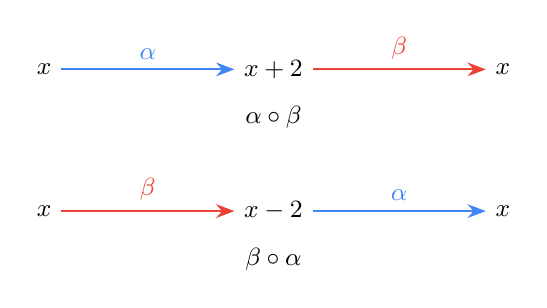
\begin{tikzpicture}[>=Stealth, font=\small, node distance=2.2cm]
  % alpha then beta
  \node (x1) {$x$};
  \node[right=of x1] (y1) {$x+2$};
  \node[right=of y1] (z1) {$x$};
  \draw[->, thick, setA] (x1) -- node[above]{$\alpha$} (y1);
  \draw[->, thick, setB] (y1) -- node[above]{$\beta$} (z1);
  \node[below=3pt of y1] {\small $\alpha \circ \beta$};

  % beta then alpha
  \begin{scope}[yshift=-1.8cm]
  \node (x2) {$x$};
  \node[right=of x2] (y2) {$x-2$};
  \node[right=of y2] (z2) {$x$};
  \draw[->, thick, setB] (x2) -- node[above]{$\beta$} (y2);
  \draw[->, thick, setA] (y2) -- node[above]{$\alpha$} (z2);
  \node[below=3pt of y2] {\small $\beta \circ \alpha$};
  \end{scope}
\end{tikzpicture}
\end{center}

\subsection*{Արտապատկերման դիագրամ վերջավոր օրինակի համար}

Հետագա ինտուիցիայի համար դիտարկենք կոնկրետ վերջավոր օրինակ։
Դիցուք $X = \{1,2,3\}$, $Y = \{a,b\}$, $Z = \{p,q\}$, որտեղ
\[
  R = \{(1,a),\;(2,b),\;(3,a)\} \subseteq X \times Y,
  \qquad
  S = \{(a,p),\;(b,q)\} \subseteq Y \times Z:
\]
Այդ դեպքում $R \circ S$-ը կապում է յուրաքանչյուր $x \in X$-ը յուրաքանչյուր $z \in Z$-ի հետ, որը հասանելի է ինչ-որ միջանկյալ $y$-ի միջոցով։
\[
  \boxed{R \circ S = \{(1,p),\;(2,q),\;(3,p)\}։}
\]

\begin{center}
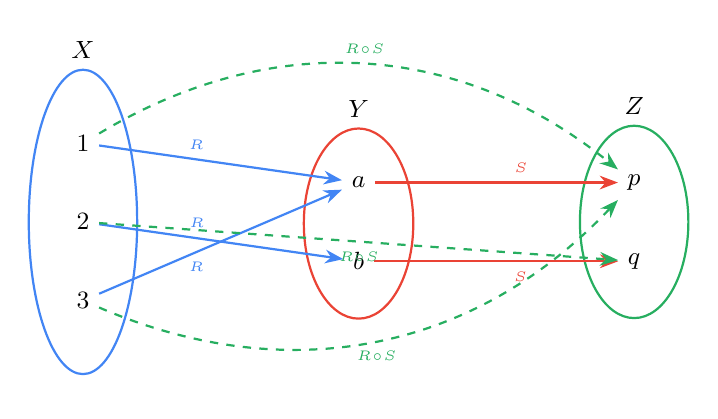
\begin{tikzpicture}[>=Stealth, node distance=0.8cm, font=\small]
  % Set X
  \node (x1) at (0, 2)   {$1$};
  \node (x2) at (0, 1)   {$2$};
  \node (x3) at (0, 0)   {$3$};
  \node[draw=setA, ellipse, thick, fit=(x1)(x2)(x3),
        inner xsep=8pt, inner ysep=4pt, label={above:$X$}] {};

  % Set Y
  \node (ya) at (3.5, 1.5) {$a$};
  \node (yb) at (3.5, 0.5) {$b$};
  \node[draw=setB, ellipse, thick, fit=(ya)(yb),
        inner xsep=8pt, inner ysep=4pt, label={above:$Y$}] {};

  % Set Z
  \node (zp) at (7, 1.5) {$p$};
  \node (zq) at (7, 0.5) {$q$};
  \node[draw=newEdge, ellipse, thick, fit=(zp)(zq),
        inner xsep=8pt, inner ysep=4pt, label={above:$Z$}] {};

  % Relation R (X -> Y)
  \draw[->, thick, setA] (x1) -- node[above, pos=0.4]{\tiny $R$} (ya);
  \draw[->, thick, setA] (x2) -- node[above, pos=0.4]{\tiny $R$} (yb);
  \draw[->, thick, setA] (x3) -- node[below, pos=0.4]{\tiny $R$} (ya);

  % Relation S (Y -> Z)
  \draw[->, thick, setB] (ya) -- node[above, pos=0.6]{\tiny $S$} (zp);
  \draw[->, thick, setB] (yb) -- node[below, pos=0.6]{\tiny $S$} (zq);

  % Composition paths (dashed, green)
  \draw[->, thick, newEdge, dashed, bend left=35]
    (x1) to node[above, pos=0.5]{\tiny $R\!\circ\!S$} (zp);
  \draw[->, thick, newEdge, dashed, bend right=0]
    (x2) to node[below, pos=0.5]{\tiny $R\!\circ\!S$} (zq);
  \draw[->, thick, newEdge, dashed, bend right=35]
    (x3) to node[below, pos=0.5]{\tiny $R\!\circ\!S$} (zp);
\end{tikzpicture}
\end{center}

{\small\textbf{Դիագրամի ընթերցում.} Հոծ կապույտ սլաքները $R$-ն են, հոծ կարմիր սլաքները՝ $S$-ը, իսկ կետագծված կանաչ սլաքները՝ $R \circ S$-ի կոմպոզիցիոն զույգերը։ Յուրաքանչյուր կետագծված սլաք ներկայացնում է կապակցված ճանապարհ $Y$-ի որևէ միջանկյալ գագաթի միջոցով:}

% ══════════════════════════════════════════════════════════════════
\newpage
\section{Խնդիր 4.1 — Հարաբերությունների հատկություններ}
% ══════════════════════════════════════════════════════════════════

\begin{theorybox}[Հարաբերությունների հատկություններ]
$A$ բազմության վրա $\alpha$ հարաբերությունը կարող է բավարարել։
\begin{itemize}[nosep]
  \item \textbf{Ռեֆլեքսիվ.} $\forall x \in A:\; (x,x) \in \alpha$:
  \item \textbf{Սիմետրիկ.} $(x,y) \in \alpha \;\Rightarrow\; (y,x) \in \alpha$:
  \item \textbf{Հակասիմետրիկ.} $(x,y) \in \alpha \;\land\; (y,x) \in \alpha \;\Rightarrow\; x = y$:
  \item \textbf{Տրանզիտիվ.} $(x,y) \in \alpha \;\land\; (y,z) \in \alpha \;\Rightarrow\; (x,z) \in \alpha$:
\end{itemize}
Նշում. սիմետրիկը և հակասիմետրիկը մեկը մյուսի ժխտումը \emph{չեն}։ հարաբերությունը կարող է լինել երկուսն էլ (օր.՝ $\Delta_A$) կամ ոչ մեկը։
\end{theorybox}

\begin{problembox}
Որոշեք, թե որ հատկություններին է բավարարում հետևյալ հարաբերություններից յուրաքանչյուրը։
\end{problembox}

%────────────────────────────────────────
\subsection*{(a)\; $\alpha = \{(x,y) \in \R^2 \mid x^2 + y^2 = 1\}$}

Երկրաչափորեն, $(x,y) \in \alpha$, եթե և միայն եթե $(x,y)$ կետը գտնվում է միավոր շրջանագծի վրա։

\begin{center}
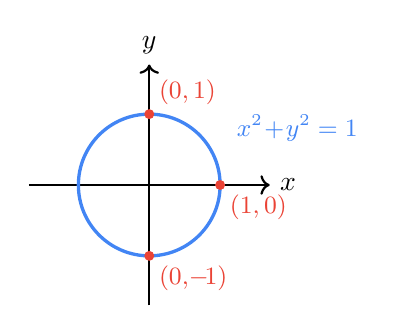
\begin{tikzpicture}[scale=0.9]
  \draw[->, thick] (-1.7,0) -- (1.7,0) node[right] {$x$};
  \draw[->, thick] (0,-1.7) -- (0,1.7) node[above] {$y$};
  \draw[setA, very thick] (0,0) circle (1);
  \fill[setB] (1,0) circle (2pt) node[below right]{\small $(1,0)$};
  \fill[setB] (0,1) circle (2pt) node[above right]{\small $(0,1)$};
  \fill[setB] (0,-1) circle (2pt) node[below right]{\small $(0,\!-\!1)$};
  \node[setA, right] at (1.1, 0.8) {\small $x^2\!+\!y^2=1$};
\end{tikzpicture}
\end{center}

\textbf{Ռեֆլեքսի՞վ։} Ոչ։ Մեզ պետք է $2x^2 = 1$ \emph{բոլոր} $x$-երի համար, ինչը չի բավարարվում $x = 0$-ի դեպքում:

\textbf{Սիմետրի՞կ։} Այո։ $x^2 + y^2 = y^2 + x^2$: \checkmark

\textbf{Հակասիմետրի՞կ։} Ոչ։ $(0, 1) \in \alpha$ և $(1, 0) \in \alpha$, բայց $0 \ne 1$:

\textbf{Տրանզիտի՞վ։} Ոչ։ $(1, 0)$ և $(0, 1) \in \alpha$, բայց $(1, 1) \notin \alpha$, քանի որ $1 + 1 = 2 \ne 1$:

\begin{answerbox}
Միայն սիմետրիկ։
\end{answerbox}

\begin{center}
\renewcommand{\arraystretch}{1.15}
\begin{tabular}{l|c|l}
  \toprule
  \textbf{Հատկություն} & \textbf{Բավարարո՞ւմ է} & \textbf{Հիմնավորում} \\
  \midrule
  Ռեֆլեքսիվ      & Ոչ  & $(0,0)$: $0^2+0^2=0\ne1$ \\
  Սիմետրիկ      & Այո & $x^2+y^2 = y^2+x^2$ \\
  Հակասիմետրիկ  & Ոչ  & $(0,1)$ և $(1,0)$ երկուսն էլ $\in\alpha$, բայց $0\ne1$ \\
  Տրանզիտիվ     & Ոչ  & $(1,0),(0,1)\in\alpha$ բայց $(1,1)\notin\alpha$ \\
  \midrule
  \textbf{Դասակարգում} & \multicolumn{2}{l}{Ոչ համարժեքության հարաբերություն, ոչ մասնակի կարգ} \\
  \bottomrule
\end{tabular}
\end{center}

%────────────────────────────────────────
\subsection*{(b)\; $\alpha = \{(x,y) \in \R^2 \mid x^2 = y^2\}$}

Համարժեքորեն $|x| = |y|$, ուստի $y = \pm x$.

\textbf{Ռեֆլեքսի՞վ։} Այո։ $x^2 = x^2$ միշտ տեղի ունի։ \checkmark

\textbf{Սիմետրի՞կ։} Այո։ $x^2 = y^2 \Rightarrow y^2 = x^2$: \checkmark

\textbf{Հակասիմետրի՞կ։} Ոչ։ $1^2 = (-1)^2$ և $(-1)^2 = 1^2$, բայց $1 \ne -1$:

\textbf{Տրանզիտի՞վ։} Այո։ $x^2 = y^2$ և $y^2 = z^2$ հետևում է $x^2 = z^2$: \checkmark

\begin{answerbox}
Ռեֆլեքսիվ, սիմետրիկ, տրանզիտիվ — սա \textbf{համարժեքության հարաբերություն} է։

Համարժեքության դասեր. $[x] = \{x, -x\}$ յուրաքանչյուր $x \in \R$-ի համար։
\end{answerbox}

\begin{center}
\renewcommand{\arraystretch}{1.15}
\begin{tabular}{l|c|l}
  \toprule
  \textbf{Հատկություն} & \textbf{Բավարարո՞ւմ է} & \textbf{Հիմնավորում} \\
  \midrule
  Ռեֆլեքսիվ      & Այո & $x^2 = x^2$ միշտ \\
  Սիմետրիկ      & Այո & $x^2=y^2 \Rightarrow y^2=x^2$ \\
  Հակասիմետրիկ  & Ոչ  & $1^2=(-1)^2$ և $(-1)^2=1^2$, բայց $1\ne -1$ \\
  Տրանզիտիվ     & Այո & $x^2=y^2, y^2=z^2 \Rightarrow x^2=z^2$ \\
  \midrule
  \textbf{Դասակարգում} & \multicolumn{2}{l}{\textbf{Համարժեքության հարաբերություն}} \\
  \bottomrule
\end{tabular}
\end{center}

\smallskip
\textbf{Մակածված տրոհում.}\; $\R$-ը տրոհվում է $\{x,-x\}$ բլոկների։ $x=0$-ի համար բլոկը $\{0\}$-ն է; $x\ne 0$-ի համար յուրաքանչյուր բլոկ ունի ճիշտ երկու տարր։

%────────────────────────────────────────
\subsection*{(c)\; $\alpha = \{(x,y) \in \Z^2 \mid x \le y\}$}

\textbf{Ռեֆլեքսի՞վ։} Այո։ $x \le x$ բոլոր $x \in \Z$-ի համար։ \checkmark

\textbf{Սիմետրի՞կ։} Ոչ։ $1 \le 2$ բայց $2 \nleq 1$:

\textbf{Հակասիմետրի՞կ։} Այո։ Եթե $x \le y$ և $y \le x$, ապա $x=y$: \checkmark

\textbf{Տրանզիտի՞վ։} Այո։ Եթե $x \le y$ և $y \le z$, ապա $x \le z$: \checkmark

\begin{answerbox}
Ռեֆլեքսիվ, հակասիմետրիկ, տրանզիտիվ — սա \textbf{մասնակի կարգ} է։ Փաստացի, այն \textbf{գծային (լրիվ) կարգ} է $\Z$-ի վրա։
\end{answerbox}

\begin{center}
\renewcommand{\arraystretch}{1.15}
\begin{tabular}{l|c|l}
  \toprule
  \textbf{Հատկություն} & \textbf{Բավարարո՞ւմ է} & \textbf{Հիմնավորում} \\
  \midrule
  Ռեֆլեքսիվ      & Այո & $x \le x$ \\
  Սիմետրիկ      & Ոչ  & $1\le 2$ բայց $2\nleq 1$ \\
  Հակասիմետրիկ  & Այո & $x\le y\land y\le x \Rightarrow x=y$ \\
  Տրանզիտիվ     & Այո & $x\le y\le z \Rightarrow x\le z$ \\
  \midrule
  \textbf{Դասակարգում} & \multicolumn{2}{l}{Գծային (լրիվ) կարգ $\Z$-ի վրա} \\
  \bottomrule
\end{tabular}
\end{center}

%────────────────────────────────────────
\subsection*{(d)\; $\alpha = \{(x,y) \in \N^2 \mid x \le y\}$}

Նույնը (c) մասի հետ, բայց սահմանափակված $\N = \{1, 2, 3, \dots\}$-ով։

\textbf{Ռեֆլեքսի՞վ։} Այո։ $x \le x$: \checkmark

\textbf{Սիմետրի՞կ։} Ոչ։ $1 \le 2$ բայց $2 \nleq 1$:

\textbf{Հակասիմետրի՞կ։} Այո։ Եթե $x \le y$ և $y \le x$, ապա $x=y$: \checkmark

\textbf{Տրանզիտի՞վ։} Այո։ Եթե $x \le y$ և $y \le z$, ապա $x \le z$: \checkmark

\begin{answerbox}
Ռեֆլեքսիվ, հակասիմետրիկ, տրանզիտիվ — սա \textbf{մասնակի կարգ} է։ Փաստացի, այն \textbf{գծային (լրիվ) կարգ} է $\N$-ի վրա։
\end{answerbox}

\begin{center}
\renewcommand{\arraystretch}{1.15}
\begin{tabular}{l|c|l}
  \toprule
  \textbf{Հատկություն} & \textbf{Բավարարո՞ւմ է} & \textbf{Հիմնավորում} \\
  \midrule
  Ռեֆլեքսիվ      & Այո & $x \le x$ \\
  Սիմետրիկ      & Ոչ  & $1\le 2$ բայց $2\nleq 1$ \\
  Հակասիմետրիկ  & Այո & $x\le y\land y\le x \Rightarrow x=y$ \\
  Տրանզիտիվ     & Այո & $x\le y\le z \Rightarrow x\le z$ \\
  \midrule
  \textbf{Դասակարգում} & \multicolumn{2}{l}{Գծային (լրիվ) կարգ $\N$-ի վրա} \\
  \bottomrule
\end{tabular}
\end{center}

%────────────────────────────────────────
\subsection*{(e)\; $\alpha = \{(x,y) \in \N^2 \mid \gcd(x,y) = 1\}$}

$(x,y) \in \alpha$ եթե և միայն եթե $x$-ը և $y$-ը փոխադարձաբար պարզ են։

\textbf{Ռեֆլեքսի՞վ։} Ոչ։ $\gcd(2,2) = 2 \ne 1$:

\textbf{Սիմետրի՞կ։} Այո։ $\gcd(x,y) = \gcd(y,x)$: \checkmark

\textbf{Հակասիմետրի՞կ։} Ոչ։ $\gcd(2,3) = 1$ և $\gcd(3,2) = 1$, բայց $2 \ne 3$:

\textbf{Տրանզիտի՞վ։} Ոչ։ $\gcd(2,3) = 1$ և $\gcd(3,4) = 1$, բայց $\gcd(2,4) = 2 \ne 1$:

\begin{answerbox}
Միայն սիմետրիկ։
\end{answerbox}

\begin{center}
\renewcommand{\arraystretch}{1.15}
\begin{tabular}{l|c|l}
  \toprule
  \textbf{Հատկություն} & \textbf{Բավարարո՞ւմ է} & \textbf{Հիմնավորում} \\
  \midrule
  Ռեֆլեքսիվ      & Ոչ  & $\gcd(2,2)=2\ne 1$ \\
  Սիմետրիկ      & Այո & $\gcd(x,y)=\gcd(y,x)$ \\
  Հակասիմետրիկ  & Ոչ  & $\gcd(2,3)=1$ և $\gcd(3,2)=1$, բայց $2\ne 3$ \\
  Տրանզիտիվ     & Ոչ  & $\gcd(2,3)=1,\;\gcd(3,4)=1$, բայց $\gcd(2,4)=2$ \\
  \midrule
  \textbf{Դասակարգում} & \multicolumn{2}{l}{Ոչ համարժեքության հարաբերություն, ոչ մասնակի կարգ} \\
  \bottomrule
\end{tabular}
\end{center}

%────────────────────────────────────────
\subsection*{(f)\; $\alpha = \{(x,y) \in \Z^2 \mid \gcd(x,y) = 1\}$}

Վերլուծությունը նույնական է (e) մասի հետ, քանի որ $\gcd$-ն կախված է միայն բացարձակ արժեքներից։ Նույն հակաօրինակները կիրառելի են։

\begin{answerbox}
Միայն սիմետրիկ։
\end{answerbox}

\begin{center}
\renewcommand{\arraystretch}{1.15}
\begin{tabular}{l|c|l}
  \toprule
  \textbf{Հատկություն} & \textbf{Բավարարո՞ւմ է} & \textbf{Հիմնավորում} \\
  \midrule
  Ռեֆլեքսիվ      & Ոչ  & $\gcd(2,2)=2\ne 1$ \\
  Սիմետրիկ      & Այո & $\gcd(x,y)=\gcd(y,x)$ \\
  Հակասիմետրիկ  & Ոչ  & $\gcd(2,3)=1$ և $\gcd(3,2)=1$, բայց $2\ne 3$ \\
  Տրանզիտիվ     & Ոչ  & $\gcd(2,3)=1,\;\gcd(3,4)=1$, բայց $\gcd(2,4)=2$ \\
  \midrule
  \textbf{Դասակարգում} & \multicolumn{2}{l}{Ոչ համարժեքության հարաբերություն, ոչ մասնակի կարգ} \\
  \bottomrule
\end{tabular}
\end{center}

%────────────────────────────────────────
\subsection*{Ամփոփիչ աղյուսակ}

\begin{center}
\renewcommand{\arraystretch}{1.3}
\begin{tabular}{l c c c c l}
  \toprule
  \textbf{Հարաբերություն} & \textbf{Ռեֆլ.} & \textbf{Սիմ.} & \textbf{Հակաս.} & \textbf{Տրանզ.} & \textbf{Տիպ} \\
  \midrule
  (a)\; $x^2+y^2=1$ ($\R$)    & —  & \checkmark & —  & — & — \\
  (b)\; $x^2=y^2$ ($\R$)      & \checkmark & \checkmark & — & \checkmark & համարժեքություն \\
  (c)\; $x \le y$ ($\Z$)     & \checkmark & — & \checkmark & \checkmark & գծային կարգ \\
  (d)\; $x \le y$ ($\N$)     & \checkmark & — & \checkmark & \checkmark & գծային կարգ \\
  (e)\; $\gcd=1$ ($\N$)       & —  & \checkmark & — & — & — \\
  (f)\; $\gcd=1$ ($\Z$)       & —  & \checkmark & — & — & — \\
  \bottomrule
\end{tabular}
\end{center}

\textbf{Ինչպես ստուգել (արագ թեստեր).}
\begin{itemize}[nosep]
  \item Ոչ ռեֆլեքսիվ։ գտեք մեկ $x$, որի համար $(x,x) \notin R$։
  \item Ոչ սիմետրիկ։ գտեք $(a,b) \in R$ այնպես, որ $(b,a) \notin R$։
  \item Ոչ հակասիմետրիկ։ գտեք $a \neq b$ այնպես, որ երկուսն էլ՝ $(a,b)$ և $(b,a)$, $R$-ում են։
  \item Ոչ տրանզիտիվ։ գտեք $(a,b), (b,c) \in R$ այնպես, որ $(a,c) \notin R$։
\end{itemize}

% ══════════════════════════════════════════════════════════════════
\newpage
\section{Խնդիր 7.2 — Հարաբերության փակումներ}
% ══════════════════════════════════════════════════════════════════

\begin{theorybox}[Հարաբերության փակումներ]
Դիցուք $\alpha$-ն $A$ վերջավոր բազմության վրա հարաբերություն է։
\begin{itemize}[nosep]
  \item \textbf{Ռեֆլեքսիվ փակում} $r(\alpha) = \alpha \cup \Delta_A$, որտեղ $\Delta_A = \{(x,x) \mid x \in A\}$։
  \item \textbf{Սիմետրիկ փակում} $s(\alpha) = \alpha \cup \alpha^{-1}$, որտեղ $\alpha^{-1} = \{(y,x) \mid (x,y) \in \alpha\}$։
  \item \textbf{Տրանզիտիվ փակում} $t(\alpha) = \alpha \cup \alpha^2 \cup \alpha^3 \cup \cdots$\; (բոլոր աստիճանների միավորումը մինչև նոր զույգեր չհայտնվեն)։
\end{itemize}
Փակումն ավելացնում է այն \emph{նվազագույն} զույգերը, որոնք անհրաժեշտ են տվյալ հատկությունը ձեռք բերելու համար։
\end{theorybox}

\begin{problembox}
Դիցուք $A = \{1, 2, 3, 4\}$ և $\alpha = \{(1,2),\,(3,1),\,(3,2),\,(2,4)\}$։

Գտեք $r(\alpha)$, $s(\alpha)$ և $t(\alpha)$։
\end{problembox}

\subsection*{Սկզբնական հարաբերությունը}

\begin{center}
\begin{minipage}{0.45\textwidth}\centering
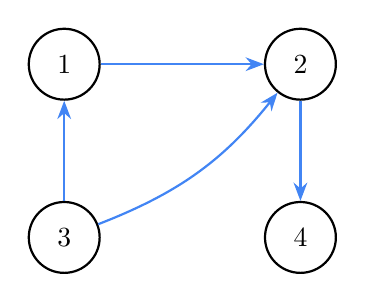
\begin{tikzpicture}[
  every node/.style={circle, draw, thick, minimum size=9mm, inner sep=0pt},
  >=Stealth
]
  \node (1) at (0,2.2)   {$1$};
  \node (2) at (3,2.2)   {$2$};
  \node (3) at (0,0)     {$3$};
  \node (4) at (3,0)     {$4$};

  \draw[->, thick, setA] (1) -- (2);
  \draw[->, thick, setA] (3) -- (1);
  \draw[->, thick, setA] (3) edge[bend right=15] (2);
  \draw[->, thick, setA] (2) -- (4);
\end{tikzpicture}
\end{minipage}%
\begin{minipage}{0.45\textwidth}\centering
$M_\alpha = \begin{pmatrix}
  0 & 1 & 0 & 0 \\
  0 & 0 & 0 & 1 \\
  1 & 1 & 0 & 0 \\
  0 & 0 & 0 & 0
\end{pmatrix}$

{\small Տողեր/սյունակներ՝ $1,2,3,4$:}
\end{minipage}
\end{center}

%────────────────────────────────────────
\subsection*{Ռեֆլեքսիվ փակում $r(\alpha)$}

Ավելացրեք բոլոր անկյունագծային զույգերը $(x,x)$՝ $x \in A$-ի համար։
\begin{align*}
  r(\alpha) &= \alpha \cup \{(1,1),\,(2,2),\,(3,3),\,(4,4)\} \\
            &= \boxed{\{(1,1),\,(1,2),\,(2,2),\,(2,4),\,(3,1),\,(3,2),\,(3,3),\,(4,4)\}։}
\end{align*}

\begin{center}
\begin{minipage}{0.45\textwidth}\centering
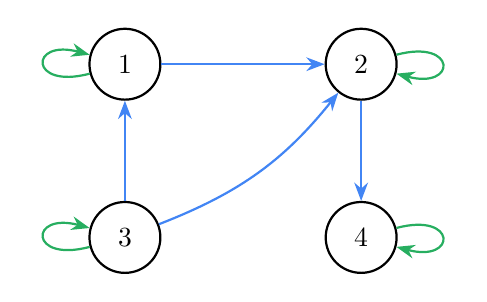
\begin{tikzpicture}[
  every node/.style={circle, draw, thick, minimum size=9mm, inner sep=0pt},
  >=Stealth
]
  \node (1) at (0,2.2)   {$1$};
  \node (2) at (3,2.2)   {$2$};
  \node (3) at (0,0)     {$3$};
  \node (4) at (3,0)     {$4$};

  % Original edges (blue)
  \draw[->, thick, setA] (1) -- (2);
  \draw[->, thick, setA] (3) -- (1);
  \draw[->, thick, setA] (3) edge[bend right=15] (2);
  \draw[->, thick, setA] (2) -- (4);
  % Added loops (green)
  \draw[->, thick, newEdge] (1) edge[loop left, looseness=8, min distance=8mm] (1);
  \draw[->, thick, newEdge] (2) edge[loop right, looseness=8, min distance=8mm] (2);
  \draw[->, thick, newEdge] (3) edge[loop left, looseness=8, min distance=8mm] (3);
  \draw[->, thick, newEdge] (4) edge[loop right, looseness=8, min distance=8mm] (4);
\end{tikzpicture}
\end{minipage}%
\begin{minipage}{0.45\textwidth}\centering
$M_{r(\alpha)} = \begin{pmatrix}
  \mathbf{1} & 1 & 0 & 0 \\
  0 & \mathbf{1} & 0 & 1 \\
  1 & 1 & \mathbf{1} & 0 \\
  0 & 0 & 0 & \mathbf{1}
\end{pmatrix}$

{\small\color{newEdge} Թավ = անկյունագծի վրա ավելացված 1-եր։}
\end{minipage}
\end{center}

%────────────────────────────────────────
\subsection*{Սիմետրիկ փակում $s(\alpha)$}

Ավելացրեք յուրաքանչյուր զույգի հակառակը։
\[
  \alpha^{-1} = \{(2,1),\,(1,3),\,(2,3),\,(4,2)\}:
\]
\[
  \boxed{s(\alpha) = \alpha \cup \alpha^{-1}
  = \{(1,2),\,(1,3),\,(2,1),\,(2,3),\,(2,4),\,(3,1),\,(3,2),\,(4,2)\}։}
\]

\begin{center}
\begin{minipage}{0.45\textwidth}\centering
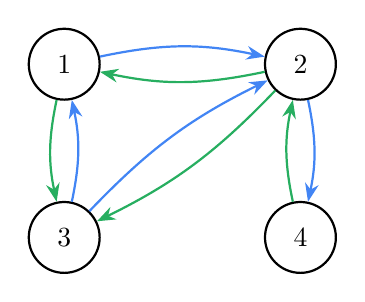
\begin{tikzpicture}[
  every node/.style={circle, draw, thick, minimum size=9mm, inner sep=0pt},
  >=Stealth
]
  \node (1) at (0,2.2)   {$1$};
  \node (2) at (3,2.2)   {$2$};
  \node (3) at (0,0)     {$3$};
  \node (4) at (3,0)     {$4$};

  % Original edges (blue) -- bend to make room for reverse
  \draw[->, thick, setA] (1) edge[bend left=12] (2);
  \draw[->, thick, setA] (3) edge[bend right=12] (1);
  \draw[->, thick, setA] (3) edge[bend left=10] (2);
  \draw[->, thick, setA] (2) edge[bend left=12] (4);
  % Added reverse edges (green)
  \draw[->, thick, newEdge] (2) edge[bend left=12] (1);
  \draw[->, thick, newEdge] (1) edge[bend right=12] (3);
  \draw[->, thick, newEdge] (2) edge[bend left=10] (3);
  \draw[->, thick, newEdge] (4) edge[bend left=12] (2);
\end{tikzpicture}
\end{minipage}%
\begin{minipage}{0.45\textwidth}\centering
$M_{s(\alpha)} = \begin{pmatrix}
  0 & 1 & \mathbf{1} & 0 \\
  \mathbf{1} & 0 & \mathbf{1} & 1 \\
  1 & 1 & 0 & 0 \\
  0 & \mathbf{1} & 0 & 0
\end{pmatrix}$

{\small\color{newEdge} Թավ = ավելացված 1-եր ($M$-ը այժմ սիմետրիկ է)։}
\end{minipage}
\end{center}

%────────────────────────────────────────
\subsection*{Տրանզիտիվ փակում $t(\alpha)$}

\textbf{Մեկնաբանություն.}\; $t(\alpha)$ տրանզիտիվ փակումը ավելացնում է բոլոր $(a,c)$ զույգերը, որոնց համար հարաբերության գրաֆում կա ուղղորդված ճանապարհ $a$-ից դեպի $c$։ Համարժեքորեն, $(a,c) \in t(\alpha)$ եթե և միայն եթե $a$-ն կարող է հասնել $c$-ին մեկ կամ ավելի քայլերով։

\medskip

\begin{tcolorbox}[colback=yellow!5, colframe=stmtFrame!80, arc=2mm,
  fonttitle=\bfseries, title={\small Տեսողական կառուցում. «Կարճ ճանապարհ» կողերի ավելացում},
  breakable, left=5pt, right=5pt, top=4pt, bottom=4pt]
Տրանզիտիվ փակումը կառուցվում է շերտ առ շերտ։ Յուրաքանչյուր քայլում մենք փնտրում ենք աճող երկարությամբ ճանապարհներ և ավելացնում ենք ուղիղ «կարճ ճանապարհ» կող յուրաքանչյուրի համար։

\begin{center}
\begin{tikzpicture}[
  every node/.style={circle, draw, thick, minimum size=9mm, inner sep=0pt},
  >=Stealth
]
  % --- Layer 0: Original relation ---
  \begin{scope}[local bounding box=L0]
    \node (a1) at (0,2.2)   {$1$};
    \node (a2) at (2.5,2.2) {$2$};
    \node (a3) at (0,0)     {$3$};
    \node (a4) at (2.5,0)   {$4$};
    \draw[->, thick, setA] (a1) -- (a2);
    \draw[->, thick, setA] (a3) -- (a1);
    \draw[->, thick, setA] (a3) edge[bend right=12] (a2);
    \draw[->, thick, setA] (a2) -- (a4);
  \end{scope}
  \node[draw=none, below=2pt of L0, font=\small\bfseries] {Քայլ 0: $\alpha$ (սկզբնական)};

  % --- Layer 1: Add length-2 shortcuts ---
  \begin{scope}[xshift=5.5cm, local bounding box=L1]
    \node (b1) at (0,2.2)   {$1$};
    \node (b2) at (2.5,2.2) {$2$};
    \node (b3) at (0,0)     {$3$};
    \node (b4) at (2.5,0)   {$4$};
    % Original edges
    \draw[->, thick, setA] (b1) -- (b2);
    \draw[->, thick, setA] (b3) -- (b1);
    \draw[->, thick, setA] (b3) edge[bend right=12] (b2);
    \draw[->, thick, setA] (b2) -- (b4);
    % New shortcut edges (length-2 paths) -- dashed red
    \draw[->, thick, setB, dashed] (b1) edge[bend left=30] (b4);
    \draw[->, thick, setB, dashed] (b3) -- (b4);
  \end{scope}
  \node[draw=none, below=2pt of L1, font=\small\bfseries] {Քայլ 1: ավելացնել $\alpha^2$ կարճ ճանապարհներ};

  % Legend
  \node[draw=none, font=\small, text width=4cm, align=left]
    at (8.8, 2.8) {%
      \textcolor{setA}{\rule{10pt}{2pt}} սկզբնական ($\alpha$)\\
      \textcolor{setB}{- - -} երկարություն-2 կարճ ճանապարհներ ($\alpha^2$)};
\end{tikzpicture}
\end{center}

\smallskip
Այս օրինակում $4$ գագաթը կլանիչ է (ելնող կողեր չկան), ուստի չկան 3 երկարությամբ ճանապարհներ, որոնք նոր զույգեր կառաջացնեն։ Գործընթացն ավարտվում է։ $t(\alpha) = \alpha \cup \alpha^2$։

Ընդհանուր դեպքում, $|A|=n$-ի համար գործընթացը միշտ ավարտվում է առավելագույնը $n-1$ քայլից հետո, քանի որ $n$-գագաթանի գրաֆում ցանկացած ճանապարհ, որը չի կրկնում գագաթները, ունի $\le n-1$ երկարություն։
\end{tcolorbox}

\medskip

Մենք հաշվարկում ենք $\alpha$-ի հաջորդական աստիճանները։

\textbf{Քայլ 1. $\alpha^2 = \alpha \circ \alpha$։}\; Յուրաքանչյուր $x \xrightarrow{\alpha} y \xrightarrow{\alpha} z$ շղթայի համար։
\begin{itemize}[nosep]
  \item $(1,2)$ և $(2,4)$։ տալիս է $\boldsymbol{(1,4)}$։  \textbf{Նոր է!}
  \item $(3,1)$ և $(1,2)$։ տալիս է $(3,2)$։  Արդեն կա $\alpha$-ում։
  \item $(3,2)$ և $(2,4)$։ տալիս է $\boldsymbol{(3,4)}$։  \textbf{Նոր է!}
\end{itemize}
Նոր զույգեր։ $\boxed{(1,4) \text{ և } (3,4)}$։

\textbf{Քայլ 2. $\alpha^3 = \alpha^2 \circ \alpha$։}\; Նոր երկրորդ կոորդինատները բոլորը $4$ են, բայց $4$-ը $\alpha$-ում չունի ելնող կողեր, ուստի այլևս նոր զույգեր չեն առաջանում։

\begin{answerbox}
$t(\alpha) = \alpha \cup \alpha^2 = \{(1,2),\;(1,4),\;(2,4),\;(3,1),\;(3,2),\;(3,4)\}։$
\end{answerbox}

\textbf{Մեկնաբանություն.} $(x, z) \in t(\alpha)$ եթե և միայն եթե սկզբնական դիգրաֆում կա ուղղորդված ճանապարհ $x$-ից դեպի $z$։

\begin{center}
\begin{minipage}{0.45\textwidth}\centering
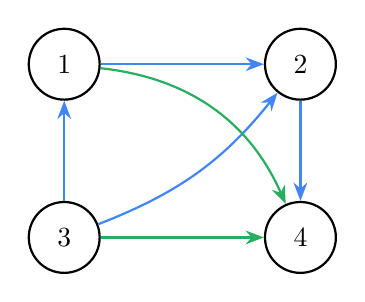
\begin{tikzpicture}[
  every node/.style={circle, draw, thick, minimum size=9mm, inner sep=0pt},
  >=Stealth
]
  \node (1) at (0,2.2)   {$1$};
  \node (2) at (3,2.2)   {$2$};
  \node (3) at (0,0)     {$3$};
  \node (4) at (3,0)     {$4$};

  % Original edges (blue)
  \draw[->, thick, setA] (1) -- (2);
  \draw[->, thick, setA] (3) -- (1);
  \draw[->, thick, setA] (3) edge[bend right=15] (2);
  \draw[->, thick, setA] (2) -- (4);
  % Added transitive edges (green)
  \draw[->, thick, newEdge] (1) edge[bend left=30] (4);
  \draw[->, thick, newEdge] (3) -- (4);
\end{tikzpicture}
\end{minipage}%
\begin{minipage}{0.45\textwidth}\centering
$M_{t(\alpha)} = \begin{pmatrix}
  0 & 1 & 0 & \mathbf{1} \\
  0 & 0 & 0 & 1 \\
  1 & 1 & 0 & \mathbf{1} \\
  0 & 0 & 0 & 0
\end{pmatrix}$

{\small\color{newEdge} Թավ = ավելացված 1-եր։}
\end{minipage}
\end{center}

\medskip

\textbf{Հասանելիության ամփոփում.}
\begin{itemize}[nosep]
  \item $1$-ից կարելի է հասնել $2$ և $4$ \;(ճանապարհ՝ $1 \to 2 \to 4$)։
  \item $2$-ից կարելի է հասնել $4$։
  \item $3$-ից կարելի է հասնել $1$, $2$, և $4$ \;(ճանապարհ՝ $3 \to 1 \to 2 \to 4$)։
  \item $4$-ից ելնող կողեր չկան — $4$-ը \emph{կլանիչ} է։
\end{itemize}

\end{document}
\newpage

% ── Practice 4 ───────────────────────────────────────────────────
\section{Գործնական 4 — Ֆունկցիաներ}
\documentclass[12pt, a4paper]{article}

% ── Packages ──────────────────────────────────────────────────────
\usepackage{fontspec}
\setmainfont{Sylfaen}
\usepackage{amsmath, amssymb, amsthm}
\renewcommand\proofname{Ապացույց}
\usepackage{mathtools}
\usepackage{enumitem}
\usepackage{tikz}
\usetikzlibrary{calc, positioning, arrows.meta, fit, patterns, decorations.pathreplacing}
\usepackage{geometry}
\geometry{margin=2.4cm}
\usepackage{xcolor}
\usepackage{tcolorbox}
\tcbuselibrary{theorems, skins, breakable}
\usepackage{booktabs}
\usepackage{hyperref}
\hypersetup{colorlinks=true, linkcolor=blue!60!black, urlcolor=blue!60!black}

\setlength{\parindent}{0pt}
\setlength{\parskip}{6pt}

% ── Colours ───────────────────────────────────────────────────────
\definecolor{setA}{RGB}{66, 133, 244}   % blue
\definecolor{setB}{RGB}{234, 67, 53}    % red
\definecolor{setC}{RGB}{251, 188, 4}    % yellow
\definecolor{theoryBg}{RGB}{232, 245, 253}
\definecolor{theoryFrame}{RGB}{66, 133, 244}
\definecolor{stmtBg}{RGB}{255, 243, 224}
\definecolor{stmtFrame}{RGB}{230, 126, 34}
\definecolor{ansBg}{RGB}{232, 250, 232}
\definecolor{ansFrame}{RGB}{39, 174, 96}

% ── Environments ──────────────────────────────────────────────────
\newtcolorbox{theorybox}[1][]{%
  colback=theoryBg, colframe=theoryFrame,
  fonttitle=\bfseries, title={\small Տեսության ամփոփում. #1},
  breakable, enhanced, arc=2mm,
  left=5pt, right=5pt, top=5pt, bottom=5pt
}

\newtcolorbox{problembox}{%
  colback=stmtBg, colframe=stmtFrame,
  fonttitle=\bfseries, title={\small Խնդրի դրվածք},
  breakable, enhanced, arc=2mm,
  left=5pt, right=5pt, top=5pt, bottom=5pt
}

\newtcolorbox{answerbox}{%
  colback=ansBg, colframe=ansFrame,
  arc=2mm, left=5pt, right=5pt, top=3pt, bottom=3pt
}

\newcommand{\Z}{\mathbb{Z}}
\newcommand{\R}{\mathbb{R}}
\newcommand{\N}{\mathbb{N}}
\newcommand{\Q}{\mathbb{Q}}
\newcommand{\powset}[1]{2^{#1}}
\newcommand{\comp}[1]{\overline{#1}}
\newcommand{\symdiff}{\mathbin{\triangle}}

% ── Title ─────────────────────────────────────────────────────────
\title{\textbf{Գործնական 4 — Ֆունկցիաներ (արտապատկերումներ)}\\[4pt]
       \large Ընտրված խնդիրների լուծումներ\\[2pt]
       \normalsize Խնդիրներ 2, 4, 5, 6, 10, 12, 19, 22, 24, 25}
\author{Դիսկրետ մաթեմատիկա — ԵՊՀ}
\date{}

\begin{document}
\maketitle
\tableofcontents
\newpage

% ══════════════════════════════════════════════════════════════════
\section{Խնդիր 2 — Իրական ֆունկցիաների որոշման և արժեքների տիրույթներ}
% ══════════════════════════════════════════════════════════════════

\begin{theorybox}[Որոշման և Արժեքների տիրույթներ]
$f(x) = \ldots$ բանաձևով տրված $f : \R \to \R$ ֆունկցիայի համար․
\begin{itemize}[nosep]
  \item \textbf{Որոշման տիրույթը}՝ $\operatorname{Dom}(f)$-ը, բոլոր այն $x \in \R$ թվերի բազմությունն է,
        որոնց համար բանաձևը իմաստ ունի (բաժանում զրոյի վրա չկա, բացասական թվից քառակուսի արմատ չկա, և այլն)։
  \item \textbf{Արժեքների տիրույթը}՝ $\operatorname{Ran}(f) = \{f(x) \mid x \in \operatorname{Dom}(f)\}$-ը, 
        այն բոլոր արժեքների բազմությունն է, որոնք ֆունկցիան փաստացի ընդունում է։
\end{itemize}

\medskip
\textbf{Հաճախ հանդիպող սահմանափակումներ.}
\begin{center}
\renewcommand{\arraystretch}{1.3}
\begin{tabular}{lll}
\toprule
\textbf{Արտահայտություն} & \textbf{Սահմանափակում} & \textbf{Պատճառ} \\
\midrule
$\sqrt{g(x)}$ & $g(x) \ge 0$ & բացասական թվի արմատը անորոշ է $\R$-ում \\
$1/g(x)$ & $g(x) \neq 0$ & բաժանում զրոյի վրա անթույլատրելի է \\
$1/\sqrt{g(x)}$ & $g(x) > 0$ & երկու սահմանափակումները միասին \\
\bottomrule
\end{tabular}
\end{center}
\end{theorybox}

\begin{problembox}
Դիցուք $f : \R \to \R$։ Գտեք հետևյալ ֆունկցիաների որոշման և արժեքների տիրույթները․
\begin{enumerate}[label=(\alph*), nosep]
  \item $f(x) = x^2 + 3$
  \item $f(x) = \sqrt{x+2}$
  \item $f(x) = \dfrac{1}{\sqrt{x-2}}$
  \item $f(x) = |x|$
  \item $f(x) = \dfrac{1}{x^2+2}$
  \item $f(x) = \dfrac{1}{x^2-2}$
\end{enumerate}
\end{problembox}

\subsection*{Լուծում}

\textbf{Երկու քայլ յուրաքանչյուր արտապատկերման համար.}
\begin{enumerate}[nosep]
  \item \textbf{Որոշման տիրույթի ստուգում.} որոշեք, թե որտեղ է բանաձևը որոշված։
  \item \textbf{Արժեքների տիրույթի ստուգում.} որոշեք, թե որ ելքային արժեքներն են ստացվում։
\end{enumerate}

\medskip

\textbf{(a)\; $f(x) = x^2 + 3$.}

$x$-ի վրա սահմանափակումներ չկան․ ցանկացած իրական թիվ կարելի է բարձրացնել քառակուսի։
\[
  \operatorname{Dom}(f) = \R.
\]
Քանի որ $x^2 \ge 0$ բոլոր $x \in \R$-ի համար, ունենք $f(x) = x^2 + 3 \ge 3$։
Նվազագույն արժեքը՝ $3$-ը, ստացվում է $x = 0$ կետում։
Երբ $x \to \pm\infty$, $f(x) \to +\infty$, և անընդհատության շնորհիվ բոլոր $\ge 3$ արժեքները ընդունվում են։
\[
  \operatorname{Ran}(f) = [3, +\infty).
\]

\begin{answerbox}
$\operatorname{Dom}(f) = \R, \quad \operatorname{Ran}(f) = [3, +\infty).$
\end{answerbox}

\bigskip
\textbf{(b)\; $f(x) = \sqrt{x+2}$.}

Մեզ պետք է $x + 2 \ge 0$, այսինքն՝ $x \ge -2$։
\[
  \operatorname{Dom}(f) = [-2, +\infty).
\]
$x = -2$ դեպքում՝ $f(-2) = 0$։ Երբ $x \to +\infty$, $f(x) \to +\infty$։
Քանի որ $\sqrt{\cdot}$-ը անընդհատ է և ոչ բացասական․
\[
  \operatorname{Ran}(f) = [0, +\infty).
\]

\begin{answerbox}
$\operatorname{Dom}(f) = [-2, +\infty), \quad \operatorname{Ran}(f) = [0, +\infty).$
\end{answerbox}

\bigskip
\textbf{(c)\; $f(x) = \dfrac{1}{\sqrt{x-2}}$.}

Մեզ պետք է $x - 2 > 0$ (խիստ անհավասարություն․ արմատի տակը դրական է, քանի որ այն հայտարարում է), այսինքն՝ $x > 2$։
\[
  \operatorname{Dom}(f) = (2, +\infty).
\]
Երբ $x \to 2^+$՝ $\sqrt{x-2} \to 0^+$, ուստի $f(x) \to +\infty$։
Երբ $x \to +\infty$՝ $\sqrt{x-2} \to +\infty$, ուստի $f(x) \to 0^+$։
Քանի որ $f$-ը անընդհատ է և խիստ նվազող $(2, +\infty)$-ում, այն ընդունում է բոլոր դրական արժեքները․
\[
  \operatorname{Ran}(f) = (0, +\infty).
\]

\begin{answerbox}
$\operatorname{Dom}(f) = (2, +\infty), \quad \operatorname{Ran}(f) = (0, +\infty).$
\end{answerbox}

\bigskip
\textbf{(d)\; $f(x) = |x|$.}

Բացարձակ արժեքը որոշված է բոլոր իրական թվերի համար։
\[
  \operatorname{Dom}(f) = \R.
\]
Քանի որ $|x| \ge 0$ բոլոր $x$-երի համար, և $|0| = 0$, ու $|x| \to +\infty$ երբ $x \to \pm\infty$․
\[
  \operatorname{Ran}(f) = [0, +\infty).
\]

\begin{answerbox}
$\operatorname{Dom}(f) = \R, \quad \operatorname{Ran}(f) = [0, +\infty).$
\end{answerbox}

\bigskip
\textbf{(e)\; $f(x) = \dfrac{1}{x^2+2}$.}

Քանի որ $x^2 + 2 \ge 2 > 0$ բոլոր $x \in \R$-ի համար, զրոյի բաժանում չկա։
\[
  \operatorname{Dom}(f) = \R.
\]
Քանի որ $x^2 + 2 \ge 2$, ունենք $f(x) = \frac{1}{x^2+2} \le \frac{1}{2}$։
Առավելագույն արժեքը՝ $\frac{1}{2}$-ը, ստացվում է $x = 0$ կետում։
Երբ $x \to \pm\infty$, $f(x) \to 0^+$, բայց $f(x) > 0$ բոլոր $x$-երի համար։
Ըստ անընդհատության, $(0, \frac{1}{2}]$ միջակայքի բոլոր արժեքները ընդունվում են։
\[
  \operatorname{Ran}(f) = \left(0,\; \tfrac{1}{2}\right].
\]

\begin{answerbox}
$\operatorname{Dom}(f) = \R, \quad \operatorname{Ran}(f) = \bigl(0,\, \frac{1}{2}\bigr].$
\end{answerbox}

\bigskip
\textbf{(f)\; $f(x) = \dfrac{1}{x^2-2}$.}

Մեզ պետք է $x^2 - 2 \neq 0$, այսինքն՝ $x \neq \pm\sqrt{2}$։
\[
  \operatorname{Dom}(f) = \R \setminus \{-\sqrt{2},\; \sqrt{2}\}.
\]
Արժեքների տիրույթը գտնելու համար նշանակենք $y = \frac{1}{x^2 - 2}$ և լուծենք $x^2$-ու համար․
\[
  y(x^2 - 2) = 1 \implies x^2 = \frac{1}{y} + 2 = \frac{1 + 2y}{y}.
\]
Մեզ պետք է $y \neq 0$ և $x^2 = \frac{1+2y}{y} \ge 0$։

\textbf{Նշանների վերլուծություն.}\; $x^2 = \frac{1+2y}{y} \ge 0$ լուծելու համար համարիչն ու հայտարարը պետք է ունենան նույն նշանը։ $y > 0$-ի դեպքում՝ $1+2y > 0$ միշտ, ուստի բոլոր $y > 0$-ները բավարարում են։ $y < 0$-ի դեպքում՝ պետք է $1+2y < 0$, այսինքն՝ $y < -\tfrac{1}{2}$։ Հետևաբար $y \in (-\infty, -\tfrac{1}{2}) \cup (0, +\infty)$, գումարած՝ պետք է ստուգել եզրային կետերը։

$x = 0$ դեպքում՝ $f(0) = \frac{1}{-2} = -\frac{1}{2}$, ուստի $y = -\frac{1}{2}$ արժեքը ընդունվում է։
\[
  \operatorname{Ran}(f) = \left(-\infty,\; -\tfrac{1}{2}\right] \cup (0, +\infty).
\]

\begin{answerbox}
$\operatorname{Dom}(f) = \R \setminus \{-\sqrt{2},\, \sqrt{2}\}, \quad
 \operatorname{Ran}(f) = \bigl(-\infty,\, -\tfrac{1}{2}\bigr] \cup (0, +\infty).$
\end{answerbox}

% ══════════════════════════════════════════════════════════════════
\newpage
\section{Խնդիր 4 — Ֆունկցիաների կոմպոզիցիա}
% ══════════════════════════════════════════════════════════════════

\begin{theorybox}[Ֆունկցիաների կոմպոզիցիա]
Տրված $f, g : \R \to \R$ ֆունկցիաների համար $f \circ g$ \textbf{կոմպոզիցիան} սահմանվում է․
\[
  (f \circ g)(x) = f\bigl(g(x)\bigr).
\]
\textbf{Կարդացեք աջից ձախ.} նախ կիրառեք $g$-ն, հետո ստացված արդյունքի վրա կիրառեք $f$-ը։

\begin{center}
\begin{tikzpicture}[>=Stealth, font=\small, node distance=2.5cm]
  \node[draw, rounded corners, fill=setA!10, minimum width=1.4cm, minimum height=0.9cm] (X) {$x$};
  \node[draw, rounded corners, fill=setC!15, minimum width=1.4cm, minimum height=0.9cm, right=of X] (GX) {$g(x)$};
  \node[draw, rounded corners, fill=setB!10, minimum width=1.4cm, minimum height=0.9cm, right=of GX] (FGX) {$f(g(x))$};
  \draw[->, thick, setA!70!black] (X) -- (GX)
    node[midway, above, font=\footnotesize]{կիրառել $g$};
  \draw[->, thick, setB!70!black] (GX) -- (FGX)
    node[midway, above, font=\footnotesize]{կիրառել $f$};
  \draw[->, thick, gray, dashed, bend left=30] (X) to
    node[midway, below=6pt, font=\footnotesize]{$f \circ g$} (FGX);
\end{tikzpicture}
\end{center}

\textbf{Զգուշացում.} Ընդհանուր դեպքում $f \circ g \neq g \circ f$ — կոմպոզիցիան կոմուտատիվ (տեղափոխական) չէ։
\end{theorybox}

\begin{problembox}
Դիցուք $f, g : \R \to \R$։ Գտեք $f \circ g$-ն և $g \circ f$-ը, եթե․
\begin{enumerate}[label=(\alph*), nosep]
  \item $f(x) = x^2 + 1$, \quad $g(x) = x + 3$
  \item $f(x) = \sqrt{x^2 + 2}$, \quad $g(x) = x^2 + 3$
  \item $f(x) = \dfrac{1}{x}$, \quad $g(x) = 2x + 3$
\end{enumerate}
\end{problembox}

\subsection*{Լուծում}

\textbf{(a)\; $f(x) = x^2 + 1$, \;$g(x) = x + 3$.}

\[
  (f \circ g)(x) = f(g(x)) = f(x+3) = (x+3)^2 + 1 = x^2 + 6x + 9 + 1 = x^2 + 6x + 10.
\]
\[
  (g \circ f)(x) = g(f(x)) = g(x^2+1) = (x^2+1) + 3 = x^2 + 4.
\]

\begin{answerbox}
$(f \circ g)(x) = x^2 + 6x + 10, \qquad (g \circ f)(x) = x^2 + 4.$
\end{answerbox}

\bigskip
\textbf{(b)\; $f(x) = \sqrt{x^2 + 2}$, \;$g(x) = x^2 + 3$.}

\[
  (f \circ g)(x) = f(g(x)) = f(x^2 + 3) = \sqrt{(x^2+3)^2 + 2} = \sqrt{x^4 + 6x^2 + 9 + 2} = \sqrt{x^4 + 6x^2 + 11}.
\]
\[
  (g \circ f)(x) = g(f(x)) = g\!\left(\sqrt{x^2+2}\right) = \left(\sqrt{x^2+2}\right)^2 + 3 = x^2 + 2 + 3 = x^2 + 5.
\]

\begin{answerbox}
$(f \circ g)(x) = \sqrt{x^4 + 6x^2 + 11}, \qquad (g \circ f)(x) = x^2 + 5.$
\end{answerbox}

\bigskip
\textbf{(c)\; $f(x) = \dfrac{1}{x}$, \;$g(x) = 2x + 3$.}

\[
  (f \circ g)(x) = f(g(x)) = f(2x+3) = \frac{1}{2x+3}, \qquad x \neq -\tfrac{3}{2}.
\]
\[
  (g \circ f)(x) = g(f(x)) = g\!\left(\frac{1}{x}\right) = \frac{2}{x} + 3 = \frac{2 + 3x}{x}, \qquad x \neq 0.
\]

\textbf{Որոշման տիրույթի ստուգում.}\; Բանաձևը հաշվելուց հետո ստուգեք, թե որտեղ է այն որոշված․ $(g \circ f)(x)$-ի համար պահանջվում է $x \in \operatorname{Dom}(f)$ և $f(x) \in \operatorname{dom}(g)$։

\begin{answerbox}
$(f \circ g)(x) = \dfrac{1}{2x+3}\;(x \neq -\frac{3}{2}), \qquad
 (g \circ f)(x) = \dfrac{2+3x}{x}\;(x \neq 0).$
\end{answerbox}

% ══════════════════════════════════════════════════════════════════
\newpage
\section{Խնդիր 5 — Հակադարձ ֆունկցիաներ}
% ══════════════════════════════════════════════════════════════════

\begin{theorybox}[Հակադարձ ֆունկցիա]
Եթե $f : A \to B$-ն բիյեկցիա է, ապա $f$-ն ունի \textbf{հակադարձ ֆունկցիա}՝ $f^{-1} : B \to A$, որը բավարարում է․
\[
  f^{-1}(y) = x \iff f(x) = y.
\]
\textbf{$f^{-1}$-ը գտնելու ալգորիթմ.}
\begin{enumerate}[nosep]
  \item Գրեք $y = f(x)$։
  \item Լուծեք $x$-ը $y$-ի միջոցով։
  \item Փոխեք անունները․ ստացված $x$-ի արտահայտությունը $y$-ից հենց $f^{-1}(y)$-ն է։
\end{enumerate}

\textbf{Ստուգում.} $f^{-1}(f(x)) = x$ և $f(f^{-1}(y)) = y$։
\end{theorybox}

\begin{problembox}
Գտեք հակադարձ հարաբերությունը․
\begin{enumerate}[label=(\alph*), nosep]
  \item $f(x) = \dfrac{x+4}{2}$
  \item $f(x) = x^3$
  \item $f(x) = \dfrac{x-2}{x+3}$
\end{enumerate}
\end{problembox}

\subsection*{Լուծում}

\textbf{(a)\; $f(x) = \dfrac{x+4}{2}$.}

Նշանակեք $y = \frac{x+4}{2}$։ Լուծեք $x$-ի համար․
\[
  2y = x + 4 \implies x = 2y - 4.
\]
\[
  \boxed{f^{-1}(y) = 2y - 4.}
\]

\emph{Ստուգում՝}\; $f(f^{-1}(y)) = f(2y-4) = \frac{(2y-4)+4}{2} = \frac{2y}{2} = y.\;\checkmark$

$f^{-1}(f(x)) = f^{-1}\!\left(\frac{x+4}{2}\right) = 2 \cdot \frac{x+4}{2} - 4 = x + 4 - 4 = x.\;\checkmark$

\begin{answerbox}
$f^{-1}(x) = 2x - 4.$
\end{answerbox}

\bigskip
\textbf{(b)\; $f(x) = x^3$.}

Նշանակեք $y = x^3$։ Լուծեք $x$-ի համար․
\[
  x = \sqrt[3]{y} = y^{1/3}.
\]
\[
  \boxed{f^{-1}(y) = \sqrt[3]{y}.}
\]

\emph{Ստուգում՝}\; $f(f^{-1}(y)) = (\sqrt[3]{y})^3 = y.\;\checkmark$ \quad
$f^{-1}(f(x)) = \sqrt[3]{x^3} = x.\;\checkmark$

\begin{answerbox}
$f^{-1}(x) = \sqrt[3]{x}.$
\end{answerbox}

\bigskip
\textbf{(c)\; $f(x) = \dfrac{x-2}{x+3}$, \quad $x \neq -3$.}

Նշանակեք $y = \frac{x-2}{x+3}$։ Լուծեք $x$-ի համար․
\begin{align*}
  y(x+3) &= x - 2 \\
  yx + 3y &= x - 2 \\
  yx - x &= -2 - 3y \\
  x(y - 1) &= -(2 + 3y) \\
  x &= \frac{-(2+3y)}{y-1} = \frac{2+3y}{1-y}, \qquad y \neq 1.
\end{align*}
Նկատենք, որ $f(x) = 1$ հավասարումը լուծում չունի (դա կպահանջեր $x - 2 = x + 3$, այսինքն՝ $-2 = 3$), ինչը հաստատում է, որ $1 \notin \operatorname{Ran}(f)$։
\[
  \boxed{f^{-1}(y) = \frac{2 + 3y}{1 - y}, \qquad y \neq 1.}
\]

\emph{Ստուգում՝}\;
$f(f^{-1}(y)) = f\!\left(\frac{2+3y}{1-y}\right)
= \frac{\frac{2+3y}{1-y} - 2}{\frac{2+3y}{1-y} + 3}
= \frac{2+3y - 2(1-y)}{2+3y + 3(1-y)}
= \frac{2+3y-2+2y}{2+3y+3-3y}
= \frac{5y}{5} = y.\;\checkmark$

\begin{answerbox}
$f^{-1}(x) = \dfrac{2+3x}{1-x}, \quad x \neq 1.$
\end{answerbox}

\bigskip
\textbf{Նշում.}\; Այստեղ հակադարձ հարաբերությունը ստացվում է ֆունկցիա, քանի որ յուրաքանչյուր արտապատկերում բիյեկտիվ է իր արժեքների տիրույթի վրա։ Ընդհանուր դեպքում հակադարձ \emph{հարաբերությունը} միշտ գոյություն ունի, բայց այն \emph{ֆունկցիա} է միայն այն դեպքում, երբ սկզբնական արտապատկերումը ինյեկտիվ է։

% ══════════════════════════════════════════════════════════════════
\newpage
\section{Խնդիր 6 — Ինյեկտիվություն, Սյուրյեկտիվություն, Բիյեկտիվություն}
% ══════════════════════════════════════════════════════════════════

\begin{theorybox}[Ինյեկտիվ, Սյուրյեկտիվ, Բիյեկտիվ]
Դիցուք $f : A \to B$։
\begin{itemize}[nosep]
  \item \textbf{Ինյեկտիվ} (միարժեք). $f(x_1) = f(x_2) \implies x_1 = x_2$։
        Համարժեքորեն, $x_1 \neq x_2 \implies f(x_1) \neq f(x_2)$։
        \emph{Հորիզոնական գծի թեստ.} յուրաքանչյուր հորիզոնական գիծ հատում է գրաֆիկը առավելագույնը մեկ անգամ։
  \item \textbf{Սյուրյեկտիվ} (վերարժեք, «onto»). $\forall\, y \in B,\; \exists\, x \in A : f(x) = y$։
        Համարժեքորեն, $\operatorname{Ran}(f) = B$։
  \item \textbf{Բիյեկտիվ} (փոխմիարժեք). թե՛ ինյեկտիվ, թե՛ սյուրյեկտիվ։
\end{itemize}

\begin{center}
\begin{tikzpicture}[>=Stealth, font=\small]
  % Injective
  \begin{scope}[xshift=0cm]
    \node[font=\footnotesize\bfseries] at (1.2, 2.5) {Ինյեկտիվ};
    \draw[thick, rounded corners] (0, -0.3) rectangle (0.8, 2.1);
    \draw[thick, rounded corners] (1.6, -0.3) rectangle (2.4, 2.1);
    \node[font=\scriptsize] at (0.4, -0.6) {$A$};
    \node[font=\scriptsize] at (2.0, -0.6) {$B$};
    \foreach \y/\lbl in {0.3/a, 0.9/b, 1.5/c}
      \node[fill=setA!30, circle, inner sep=1.5pt, font=\tiny] (L\lbl) at (0.4, \y) {\lbl};
    \foreach \y/\lbl in {0.0/1, 0.6/2, 1.2/3, 1.8/4}
      \node[fill=setB!20, circle, inner sep=1.5pt, font=\tiny] (R\lbl) at (2.0, \y) {\lbl};
    \draw[->, thick, gray] (La) -- (R1);
    \draw[->, thick, gray] (Lb) -- (R3);
    \draw[->, thick, gray] (Lc) -- (R4);
  \end{scope}
  % Surjective
  \begin{scope}[xshift=4cm]
    \node[font=\footnotesize\bfseries] at (1.2, 2.5) {Սյուրյեկտիվ};
    \draw[thick, rounded corners] (0, -0.3) rectangle (0.8, 2.1);
    \draw[thick, rounded corners] (1.6, -0.3) rectangle (2.4, 2.1);
    \node[font=\scriptsize] at (0.4, -0.6) {$A$};
    \node[font=\scriptsize] at (2.0, -0.6) {$B$};
    \foreach \y/\lbl in {0.2/a, 0.7/b, 1.2/c, 1.7/d}
      \node[fill=setA!30, circle, inner sep=1.5pt, font=\tiny] (L\lbl) at (0.4, \y) {\lbl};
    \foreach \y/\lbl in {0.3/1, 0.9/2, 1.5/3}
      \node[fill=setB!20, circle, inner sep=1.5pt, font=\tiny] (R\lbl) at (2.0, \y) {\lbl};
    \draw[->, thick, gray] (La) -- (R1);
    \draw[->, thick, gray] (Lb) -- (R2);
    \draw[->, thick, gray] (Lc) -- (R3);
    \draw[->, thick, gray] (Ld) -- (R2);
  \end{scope}
  % Bijective
  \begin{scope}[xshift=8cm]
    \node[font=\footnotesize\bfseries] at (1.2, 2.5) {Բիյեկտիվ};
    \draw[thick, rounded corners] (0, -0.3) rectangle (0.8, 2.1);
    \draw[thick, rounded corners] (1.6, -0.3) rectangle (2.4, 2.1);
    \node[font=\scriptsize] at (0.4, -0.6) {$A$};
    \node[font=\scriptsize] at (2.0, -0.6) {$B$};
    \foreach \y/\lbl in {0.3/a, 0.9/b, 1.5/c}
      \node[fill=setA!30, circle, inner sep=1.5pt, font=\tiny] (L\lbl) at (0.4, \y) {\lbl};
    \foreach \y/\lbl in {0.3/1, 0.9/2, 1.5/3}
      \node[fill=setB!20, circle, inner sep=1.5pt, font=\tiny] (R\lbl) at (2.0, \y) {\lbl};
    \draw[->, thick, gray] (La) -- (R1);
    \draw[->, thick, gray] (Lb) -- (R2);
    \draw[->, thick, gray] (Lc) -- (R3);
  \end{scope}
\end{tikzpicture}
\end{center}
\end{theorybox}

\begin{problembox}
Որոշեք, թե հետևյալ $f : \R \to \R$ արտապատկերումներից որոնք են ինյեկտիվ, սյուրյեկտիվ կամ բիյեկտիվ.
\begin{enumerate}[label=(\alph*), nosep]
  \item $f(x) = |x|$
  \item $f(x) = x^2 + 4$
  \item $f(x) = x^3 + 6$
  \item $f(x) = x + |x|$
  \item $f(x) = x(x-2)(x+2)$
\end{enumerate}
\end{problembox}

\subsection*{Լուծում}

\textbf{Արագ թեստեր.}
\begin{itemize}[nosep]
  \item $|x|$: սիմետրիան ($f(x) = f(-x)$) անմիջապես ցույց է տալիս, որ ինյեկտիվ չէ։
  \item $x^2 + c$: պարաբոլը ունի մինիմում, ուստի սյուրյեկտիվ չէ $\mathbb{R}$-ի վրա։
  \item $x^3 + c$: խիստ մոնոտոն է, հետևաբար ինյեկտիվ է; սահմանային վարքը տալիս է սյուրյեկտիվություն։
  \item $x + |x|$: նախ վերածեք կտորային տեսքի, հետո ստուգեք յուրաքանչյուր կտորը։
  \item $x^3 - 4x$: փնտրեք կրկնվող արժեքներ (լոկալ էքստրեմումներ) և օգտագործեք սահմանային վարքը սյուրյեկտիվության համար։
\end{itemize}

\medskip

\textbf{(a)\; $f(x) = |x|$.}

\emph{Ինյեկտիվ չէ՝}\; $f(1) = |1| = 1 = |-1| = f(-1)$, բայց $1 \neq -1$։

\emph{Սյուրյեկտիվ չէ՝}\; $|x| \ge 0$ բոլոր $x$-երի համար, ուստի ոչ մի $x$ չի բավարարում $f(x) = -1$։
Արժեքների տիրույթը $[0, +\infty) \neq \R$ է։

\begin{answerbox}
$f(x) = |x|$: ոչ ինյեկտիվ է, ոչ էլ սյուրյեկտիվ (հետևաբար բիյեկտիվ չէ)։
\end{answerbox}

\bigskip
\textbf{(b)\; $f(x) = x^2 + 4$.}

\emph{Ինյեկտիվ չէ՝}\; $f(1) = 5 = f(-1)$, բայց $1 \neq -1$։

\emph{Սյուրյեկտիվ չէ՝}\; $x^2 + 4 \ge 4$ բոլոր $x$-երի համար, ուստի ոչ մի $x$ չի բավարարում $f(x) = 0$։
Արժեքների տիրույթը $[4, +\infty) \neq \R$ է։

\begin{answerbox}
$f(x) = x^2 + 4$: ոչ ինյեկտիվ է, ոչ էլ սյուրյեկտիվ (հետևաբար բիյեկտիվ չէ)։
\end{answerbox}

\bigskip
\textbf{(c)\; $f(x) = x^3 + 6$.}

\emph{Ինյեկտիվ է՝}\; Դիցուք $f(x_1) = f(x_2)$։ Այդ դեպքում $x_1^3 + 6 = x_2^3 + 6$,
ուստի $x_1^3 = x_2^3$։ Քանի որ խորանարդ ֆունկցիան խիստ աճող է $\R$-ում,
սրանից հետևում է $x_1 = x_2$։

\emph{Սյուրյեկտիվ է՝}\; Ցանկացած $y \in \R$-ի համար, մեզ պետք է $x^3 + 6 = y$, այսինքն՝
$x = \sqrt[3]{y - 6}$։ Քանի որ խորանարդ արմատը որոշված է բոլոր իրական թվերի համար, ապա
այդպիսի $x$ միշտ գոյություն ունի։

\begin{answerbox}
$f(x) = x^3 + 6$: \textbf{բիյեկտիվ} է (և՛ ինյեկտիվ, և՛ սյուրյեկտիվ)։
\end{answerbox}

\bigskip
\textbf{(d)\; $f(x) = x + |x|$.}

Նախ պարզեցնենք․
\[
  f(x) = x + |x| = \begin{cases} 2x & \text{եթե } x \ge 0, \\ 0 & \text{եթե } x < 0. \end{cases}
\]

\emph{Ինյեկտիվ չէ՝}\; $f(-1) = 0 = f(-2)$, բայց $-1 \neq -2$։
(Փաստացի, $f(x) = 0$ բոլոր $x < 0$-ների համար։)

\emph{Սյուրյեկտիվ չէ՝}\; $x \ge 0$-ի համար $f(x) = 2x \ge 0$։
$x < 0$-ի համար $f(x) = 0$։ Ուստի $f(x) \ge 0$ բոլոր $x$-երի համար,
և ոչ մի $x$ չի բավարարում $f(x) = -1$։ Արժեքների տիրույթը $[0, +\infty) \neq \R$ է։

\begin{answerbox}
$f(x) = x + |x|$: ոչ ինյեկտիվ է, ոչ էլ սյուրյեկտիվ (հետևաբար բիյեկտիվ չէ)։
\end{answerbox}

\bigskip
\textbf{(e)\; $f(x) = x(x-2)(x+2) = x^3 - 4x$.}

\emph{Ինյեկտիվ չէ՝}\; $f(0) = 0$ և $f(2) = 2 \cdot 0 \cdot 4 = 0$,
ուստի $f(0) = f(2) = 0$, բայց $0 \neq 2$։

\emph{Սյուրյեկտիվ է՝}\; $f(x) = x^3 - 4x$-ը խորանարդ բազմանդամ է դրական ավագ գործակցով։
Երբ $x \to -\infty$, $f(x) \to -\infty$, և երբ $x \to +\infty$, $f(x) \to +\infty$։
Միջանկյալ արժեքի թեորեմի համաձայն, յուրաքանչյուր $y \in \R$ ընդունվում է։

\begin{center}
\begin{tikzpicture}[scale=0.55, >=Stealth]
  \draw[->, thick] (-3.5, 0) -- (3.5, 0) node[right] {$x$};
  \draw[->, thick] (0, -5.5) -- (0, 5.5) node[above] {$y$};

  % The cubic curve
  \draw[very thick, setA, domain=-2.8:2.8, samples=100, smooth]
    plot (\x, {(\x)*(\x-2)*(\x+2)*0.6});
  \node[setA, right] at (2.5, 4) {\small $f(x) = x^3 - 4x$};

  % Horizontal line y=0 hitting 3 points (not injective)
  \draw[thick, setB, dashed] (-3.2, 0) -- (3.2, 0);
  \fill[setB] (-2, 0) circle (4pt);
  \fill[setB] (0, 0) circle (4pt);
  \fill[setB] (2, 0) circle (4pt);
  \node[setB, below, font=\scriptsize] at (-2, -0.3) {$-2$};
  \node[setB, below left, font=\scriptsize] at (0, -0.3) {$0$};
  \node[setB, below, font=\scriptsize] at (2, -0.3) {$2$};

  % Annotations
  \node[font=\scriptsize, setB!70!black, align=center] at (-3, 2.5) {$y=0$ հատում է\\3 կետերում․\\ինյեկտիվ չէ};

  % Show surjectivity: arrows to ±∞
  \draw[->, thick, gray] (2.6, 4.5) -- (2.8, 5.2);
  \draw[->, thick, gray] (-2.6, -4.5) -- (-2.8, -5.2);
  \node[font=\scriptsize, gray, right] at (2.6, 5.0) {$\to +\infty$};
  \node[font=\scriptsize, gray, left] at (-2.6, -5.0) {$\to -\infty$};

  % Tick marks
  \foreach \y in {-4,-2,2,4} {
    \draw (0.1, \y*0.6) -- (-0.1, \y*0.6);
  }
\end{tikzpicture}
\end{center}

\begin{answerbox}
$f(x) = x(x-2)(x+2)$: սյուրյեկտիվ է, բայց \textbf{ոչ ինյեկտիվ} (հետևաբար բիյեկտիվ չէ)։
\end{answerbox}

% ══════════════════════════════════════════════════════════════════
\newpage
\section{Խնդիր 10 — Արտապատկերման միջուկը համարժեքության հարաբերություն է}
% ══════════════════════════════════════════════════════════════════

\begin{theorybox}[Արտապատկերման միջուկ (Kernel)]
Դիցուք $f : A \to B$ արտապատկերում է։ $f$-ի \textbf{միջուկը} հարաբերություն է $A$-ի վրա, որը սահմանվում է հետևյալ կերպ․
\[
  \operatorname{Ker}(f) = \{(a_1, a_2) \in A \times A \mid f(a_1) = f(a_2)\}.
\]
Մենք գրում ենք $a_1 \sim a_2$, եթե $(a_1, a_2) \in \operatorname{Ker}(f)$, այսինքն՝ $f(a_1) = f(a_2)$։

\medskip
\textbf{Համարժեքության հարաբերությունը} $A$-ի վրա այն $\sim$ հարաբերությունն է, որը․
\begin{enumerate}[nosep]
  \item \textbf{Ռեֆլեքսիվ է.} $a \sim a$ բոլոր $a \in A$-երի համար։
  \item \textbf{Սիմետրիկ է.} $a \sim b \implies b \sim a$։
  \item \textbf{Տրանզիտիվ է.} $a \sim b \land b \sim c \implies a \sim c$։
\end{enumerate}

\begin{center}
\begin{tikzpicture}[>=Stealth, font=\small]
  \draw[thick, rounded corners] (0, 0) rectangle (2.2, 3.2);
  \draw[thick, rounded corners] (3.8, 0) rectangle (6.0, 3.2);
  \node[font=\footnotesize\bfseries] at (1.1, -0.3) {$A$};
  \node[font=\footnotesize\bfseries] at (4.9, -0.3) {$B$};

  \node[fill=setA!30, circle, inner sep=1.5pt, font=\tiny] (a1) at (0.7, 2.5) {$a_1$};
  \node[fill=setA!30, circle, inner sep=1.5pt, font=\tiny] (a2) at (0.7, 1.6) {$a_2$};
  \node[fill=setA!30, circle, inner sep=1.5pt, font=\tiny] (a3) at (1.5, 2.1) {$a_3$};
  \node[fill=setA!15, circle, inner sep=1.5pt, font=\tiny] (a4) at (1.1, 0.7) {$a_4$};

  \node[fill=setB!20, circle, inner sep=2pt, font=\tiny] (b1) at (4.9, 2.2) {$b_1$};
  \node[fill=setB!20, circle, inner sep=2pt, font=\tiny] (b2) at (4.9, 0.8) {$b_2$};

  \draw[->, thick, gray] (a1) -- (b1);
  \draw[->, thick, gray] (a2) -- (b1);
  \draw[->, thick, gray] (a3) -- (b1);
  \draw[->, thick, gray] (a4) -- (b2);

  % equivalence class brace
  \draw[decorate, decoration={brace, amplitude=5pt, mirror}, setA!70!black]
    (0.3, 1.3) -- (0.3, 2.8)
    node[midway, left=6pt, font=\tiny, align=right]{նույն\\պատկերը};
\end{tikzpicture}
\end{center}
$\operatorname{Ker}(f)$-ի համարժեքության դասերը ճշգրտորեն համընկնում են $b \in \operatorname{Ran}(f)$-ի
\textbf{շերտերի} (fibers) հետ՝ $f^{-1}(\{b\}) = \{a \in A \mid f(a) = b\}$։
\end{theorybox}

\begin{problembox}
Ապացուցեք, որ ցանկացած $f : A \to B$ արտապատկերման համար, նրա միջուկը՝ $\operatorname{Ker}(f)$-ը, համարժեքության հարաբերություն է $A$-ի վրա։
\end{problembox}

\subsection*{Լուծում}

Մենք պետք է ստուգենք համարժեքության հարաբերության երեք հատկությունները։
Հիշենք. $a_1 \sim a_2 \iff f(a_1) = f(a_2)$։

\textbf{1. Ռեֆլեքսիվություն.}\;
Դիցուք $a \in A$։ Ապա $f(a) = f(a)$ (հավասարությունը ռեֆլեքսիվ է), ուստի $a \sim a$։ \checkmark

\textbf{2. Սիմետրիկություն.}\;
Դիցուք $a_1 \sim a_2$, այսինքն՝ $f(a_1) = f(a_2)$։
Ապա $f(a_2) = f(a_1)$ (հավասարությունը սիմետրիկ է), ուստի $a_2 \sim a_1$։ \checkmark

\textbf{3. Տրանզիտիվություն.}\;
Դիցուք $a_1 \sim a_2$ և $a_2 \sim a_3$, այսինքն՝ $f(a_1) = f(a_2)$ և $f(a_2) = f(a_3)$։
Ապա $f(a_1) = f(a_3)$ (հավասարությունը տրանզիտիվ է), ուստի $a_1 \sim a_3$։ \checkmark

\medskip
Քանի որ $\operatorname{Ker}(f)$-ը ռեֆլեքսիվ է, սիմետրիկ և տրանզիտիվ, այն համարժեքության հարաբերություն է $A$-ի վրա։ \qed

\begin{answerbox}
$\operatorname{Ker}(f)$ միջուկը ժառանգում է ռեֆլեքսիվությունը, սիմետրիկությունը և տրանզիտիվությունը $B$-ի վրա «$=$» հավասարության հարաբերությունից, ուստի այն համարժեքության հարաբերություն է $A$-ի վրա։
\end{answerbox}

\bigskip
\textbf{Կոնկրետ օրինակ.}\; Եթե $f \colon \{1,2,3,4\} \to \{a,b\}$, որտեղ $f(1) = f(3) = a$ և $f(2) = f(4) = b$, ապա․
\begin{itemize}[nosep]
  \item $1$-ի համարժեքության դասը $f^{-1}(\{a\}) = \{1, 3\}$-ն է։
  \item $2$-ի համարժեքության դասը $f^{-1}(\{b\}) = \{2, 4\}$-ն է։
  \item Տրոհումը՝ $\bigl\{\{1,3\},\;\{2,4\}\bigr\}$։
\end{itemize}

% ══════════════════════════════════════════════════════════════════
\newpage
\section{Խնդիր 12 — \texorpdfstring{$f(x) = \frac{x}{2x+1}$}{f(x)=x/(2x+1)} \texorpdfstring{$\Q^+$}{Q+}-ի վրա. Ինյեկտիվ է, բայց ոչ սյուրյեկտիվ}
% ══════════════════════════════════════════════════════════════════

\begin{theorybox}[Ինյեկտիվության և Սյուրյեկտիվության ապացուցման մեթոդներ]
\textbf{Ինյեկտիվությունը ապացուցելու համար.}\;
Ենթադրեք $f(x_1) = f(x_2)$ և ցույց տվեք, որ $x_1 = x_2$ (ուղիղ ապացույց),
կամ ենթադրեք $x_1 \neq x_2$ և ցույց տվեք, որ $f(x_1) \neq f(x_2)$ (հակասող ենթադրություն)։

\textbf{Սյուրյեկտիվությունը հերքելու համար.}\;
Գտեք կոնկրետ $y$ արժեքների տիրույթում, որի համար $f(x) = y$ հավասարումը լուծում չունի որոշման տիրույթում։

\textbf{Սյուրյեկտիվությունը ապացուցելու համար.}\;
Տրված կամայական $y$-ի համար, լուծեք $f(x) = y$ և ստուգեք, որ գտնված $x$-ը պատկանում է որոշման տիրույթին։
\end{theorybox}

\begin{problembox}
Դիցուք $f : \Q^+ \to \Q^+$ սահմանված է $f(x) = \dfrac{x}{2x+1}$ բանաձևով։
Ապացուցեք, որ $f$-ը ինյեկտիվ է, բայց սյուրյեկտիվ չէ։
\end{problembox}

\subsection*{Լուծում}

\textbf{Ինտուիցիա.}\; Գրելով $f(x) = \dfrac{1}{2 + 1/x}$, տեսնում ենք, որ երբ $x$-ն աճում է $\mathbb{Q}^+$-ում, հայտարարը՝ $2 + 1/x$-ը, նվազում է, ուստի $f(x)$-ն աճում է։ Խիստ աճող ֆունկցիան միշտ ինյեկտիվ է։

\medskip

\textbf{Ինյեկտիվություն.}\;
Դիցուք $x_1, x_2 \in \Q^+$ և ենթադրենք $f(x_1) = f(x_2)$․
\[
  \frac{x_1}{2x_1 + 1} = \frac{x_2}{2x_2 + 1}.
\]
Խաչաձև բազմապատկելով (հայտարարները դրական են, քանի որ $x_1, x_2 > 0$)․
\[
  x_1(2x_2 + 1) = x_2(2x_1 + 1).
\]
Բացելով փակագծերը․
\[
  2x_1 x_2 + x_1 = 2x_1 x_2 + x_2.
\]
Երկու կողմից հանելով $2x_1 x_2$․
\[
  x_1 = x_2.
\]
Հետևաբար $f$-ը ինյեկտիվ է։ \qed

\bigskip
\textbf{Ոչ սյուրյեկտիվություն.}\;
Մենք պնդում ենք, որ $y = \frac{1}{2}$ թիվը պատկանում է $\Q^+$-ին, բայց չի պատկանում $\operatorname{Ran}(f)$-ին։

Ենթադրենք հակառակը, որ գոյություն ունի $x \in \Q^+$ այնպես, որ $f(x) = \frac{1}{2}$․
\[
  \frac{x}{2x+1} = \frac{1}{2} \implies 2x = 2x + 1 \implies 0 = 1.
\]
Սա հակասություն է։ Հետևաբար ոչ մի $x \in \Q^+$ չի բավարարում $f(x) = \frac{1}{2}$ պայմանին։

\medskip
Ավելի ընդհանուր, ցանկացած $x > 0$-ի համար․
\[
  f(x) = \frac{x}{2x+1} = \frac{1}{2 + \frac{1}{x}} < \frac{1}{2},
\]
քանի որ $\frac{1}{x} > 0$, ուստի $2 + \frac{1}{x} > 2$, և հետևաբար $\frac{1}{2+\frac{1}{x}} < \frac{1}{2}$։
Այսպիսով $\operatorname{Ran}(f) \subseteq \bigl(0, \frac{1}{2}\bigr)$, ուստի $f$-ը սյուրյեկտիվ չէ $\Q^+$-ի վրա։ \qed

\begin{answerbox}
$f(x) = \frac{x}{2x+1}$-ը $\Q^+$-ի վրա \textbf{ինյեկտիվ} է (խաչաձև բազմապատկումից),
բայց \textbf{սյուրյեկտիվ չէ} (օրինակ, $y = \frac{1}{2}$-ը $\operatorname{Ran}(f)$-ում չէ, քանի որ $f(x) < \frac{1}{2}$ բոլոր $x > 0$-ների համար)։
\end{answerbox}

% ══════════════════════════════════════════════════════════════════
\newpage
\section{Խնդիր 19 — \texorpdfstring{$f(A \cap B) = f(A) \cap f(B)$}{f(A∩B)=f(A)∩f(B)} Այն և միայն այն դեպքում, երբ \texorpdfstring{$f$}{f}-ը ինյեկտիվ է}
% ══════════════════════════════════════════════════════════════════

\begin{theorybox}[Հատումների պատկերները]
Ցանկացած $f : X \to Y$ արտապատկերման և $A, B \subseteq X$ ենթաբազմությունների համար․
\[
  f(A \cap B) \subseteq f(A) \cap f(B) \qquad\text{միշտ տեղի ունի:}
\]
Սակայն, $f(A \cap B) = f(A) \cap f(B)$ հավասարությունը \textbf{ոչ միշտ} է տեղի ունենում։
Այն տեղի ունի բոլոր $A, B \subseteq X$-երի համար այն և միայն այն դեպքում, երբ $f$-ը \textbf{ինյեկտիվ} է։

\begin{center}
\begin{tikzpicture}[>=Stealth, font=\small, scale=0.9]
  % Non-injective case
  \begin{scope}[xshift=0cm]
    \node[font=\footnotesize\bfseries] at (1.5, 2.8) {Ոչ ինյեկտիվ $f$};
    \draw[thick, rounded corners] (-0.2, -0.2) rectangle (2.2, 2.3);
    \draw[thick, rounded corners] (3.3, -0.2) rectangle (5.0, 2.3);
    \node[font=\scriptsize] at (1.0, -0.5) {$X$};
    \node[font=\scriptsize] at (4.15, -0.5) {$Y$};

    \node[fill=setA!30, circle, inner sep=1.5pt, font=\tiny] (a) at (0.5, 1.5) {$a$};
    \node[fill=setB!30, circle, inner sep=1.5pt, font=\tiny] (b) at (1.5, 1.5) {$b$};
    \node[font=\tiny, setA!70!black] at (0.5, 0.8) {$A$};
    \node[font=\tiny, setB!70!black] at (1.5, 0.8) {$B$};

    \node[fill=gray!20, circle, inner sep=2pt, font=\tiny] (y) at (4.15, 1.5) {$y$};

    \draw[->, thick, setA!70!black] (a) -- (y);
    \draw[->, thick, setB!70!black] (b) -- (y);

    \node[font=\tiny, align=center] at (1.0, 0.0) {$A \cap B = \varnothing$\\բայց $f(A)\cap f(B) = \{y\}$};
  \end{scope}
\end{tikzpicture}
\end{center}
\end{theorybox}

\begin{problembox}
Ո՞ր արտապատկերումների համար է տեղի ունենում $f(A \cap B) = f(A) \cap f(B)$ պայմանը որոշման տիրույթի բոլոր $A, B$ ենթաբազմությունների համար։

Պատասխան․ ինյեկտիվ արտապատկերումների։ Ապացուցեք երկու ուղղությամբ։
\end{problembox}

\subsection*{Լուծում}

\textbf{Ինչու է սա կարևոր.}\; Եթե $f$-ը ինյեկտիվ չէ, ասենք $f(1) = f(2) = y$, ապա $f(\{1\}) \cap f(\{2\}) = \{y\} \neq \varnothing$, բայց $\{1\} \cap \{2\} = \varnothing$։ Այսպիսով $f(A \cap B) \neq f(A) \cap f(B)$ ընդհանուր դեպքում։ Ինյեկտիվությունը հենց այն պայմանն է, որը կանխում է սա։

\medskip

\textbf{Ուղղություն 1. Եթե $f$-ը ինյեկտիվ է, ապա $f(A \cap B) = f(A) \cap f(B)$։}

$f(A \cap B) \subseteq f(A) \cap f(B)$ ներդրումը տեղի ունի ցանկացած ֆունկցիայի համար (եթե $x \in A \cap B$, ապա $f(x) \in f(A)$ և $f(x) \in f(B)$)։

Մենք ապացուցում ենք հակադարձ ներդրումը՝ $f(A) \cap f(B) \subseteq f(A \cap B)$։

Դիցուք $y \in f(A) \cap f(B)$։ Այդ դեպքում՝
\begin{itemize}[nosep]
  \item $y \in f(A)$, ուստի գոյություն ունի $a \in A$, որ $f(a) = y$։
  \item $y \in f(B)$, ուստի գոյություն ունի $b \in B$, որ $f(b) = y$։
\end{itemize}
Քանի որ $f(a) = y = f(b)$ և $f$-ը ինյեկտիվ է, եզրակացնում ենք, որ $a = b$։
Նշանակենք այս ընդհանուր տարրը $c = a = b$։ Այդ դեպքում $c \in A$ և $c \in B$, ուստի $c \in A \cap B$։
Հետևաբար $y = f(c) \in f(A \cap B)$։

Սա ցույց է տալիս, որ $f(A) \cap f(B) \subseteq f(A \cap B)$, ինչն ավարտում է հավասարության ապացույցը։ \qed

\bigskip
\textbf{Ուղղություն 2. Եթե $f(A \cap B) = f(A) \cap f(B)$ բոլոր $A, B$-երի համար, ապա $f$-ը ինյեկտիվ է։}

Մենք ապացուցում ենք հակասող ենթադրությամբ․ եթե $f$-ը ինյեկտիվ չէ, ապա գոյություն ունեն $A, B$, որոնց համար $f(A \cap B) \neq f(A) \cap f(B)$։

Ենթադրենք $f$-ը ինյեկտիվ չէ։ Այդ դեպքում գոյություն ունեն $x_1 \neq x_2$ տարրեր որոշման տիրույթում, այնպիսիք, որ $f(x_1) = f(x_2)$։
Վերցնենք $A = \{x_1\}$ և $B = \{x_2\}$։ Այդ դեպքում՝
\begin{itemize}[nosep]
  \item $A \cap B = \varnothing$ (քանի որ $x_1 \neq x_2$), ուստի $f(A \cap B) = f(\varnothing) = \varnothing$։
  \item $f(A) = \{f(x_1)\}$ և $f(B) = \{f(x_2)\} = \{f(x_1)\}$,
        ուստի $f(A) \cap f(B) = \{f(x_1)\} \neq \varnothing$։
\end{itemize}
Հետևաբար $f(A \cap B) \neq f(A) \cap f(B)$։ \qed

\begin{answerbox}
$f(A \cap B) = f(A) \cap f(B)$ տեղի ունի բոլոր $A, B$-երի համար այն և միայն այն դեպքում, երբ $f$-ը ինյեկտիվ է։
\end{answerbox}

% ══════════════════════════════════════════════════════════════════
\newpage
\section{Խնդիր 22 — Անջատ ենթաբազմություններ հավասար պատկերներով}
% ══════════════════════════════════════════════════════════════════

\begin{theorybox}[Անջատ բազմությունների պատկերները]
Եթե $f : A \to B$-ն ինյեկտիվ \textbf{չէ}, ապա տարբեր տարրեր կարող են արտապատկերվել նույն
արժեքին (պատկերին)։ Սա նշանակում է, որ որոշման տիրույթի անջատ ենթաբազմություններ կարող են
ունենալ հատվող, կամ նույնիսկ հավասար, պատկերներ։
\end{theorybox}

\begin{problembox}
Հնարավո՞ր է արդյոք, որ $f : A \to B$-ն և անջատ ու ոչ դատարկ $X_1, X_2 \subseteq A$ ենթաբազմությունները
(այսինքն՝ $X_1 \cap X_2 = \varnothing$, $X_1 \neq \varnothing$, $X_2 \neq \varnothing$)
ունենան $f(X_1) = f(X_2)$։
\end{problembox}

\subsection*{Լուծում}

\textbf{Այո}, սա հնարավոր է։ Բերենք կոնկրետ օրինակ։

Դիցուք $A = \{1, 2, 3, 4\}$, $B = \{a, b\}$, և սահմանենք $f$-ը հետևյալ կերպ․
\[
  f(1) = a, \quad f(2) = b, \quad f(3) = a, \quad f(4) = b.
\]
Վերցրեք $X_1 = \{1, 2\}$ և $X_2 = \{3, 4\}$։

\begin{center}
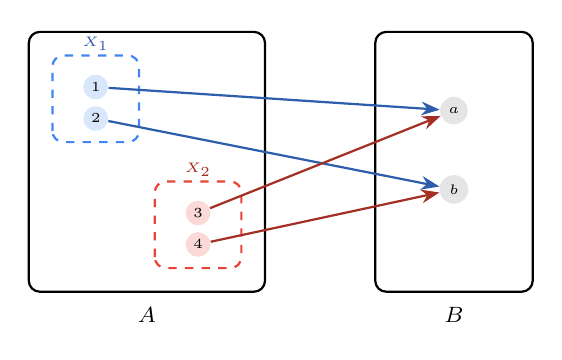
\begin{tikzpicture}[>=Stealth, font=\small]
  \draw[thick, rounded corners] (-0.2, -0.3) rectangle (2.8, 3.0);
  \draw[thick, rounded corners] (4.2, -0.3) rectangle (6.2, 3.0);
  \node[font=\footnotesize\bfseries] at (1.3, -0.6) {$A$};
  \node[font=\footnotesize\bfseries] at (5.2, -0.6) {$B$};

  % X1 box
  \draw[thick, setA, dashed, rounded corners] (0.1, 1.6) rectangle (1.2, 2.7);
  \node[font=\tiny, setA!70!black] at (0.65, 2.85) {$X_1$};
  \node[fill=setA!20, circle, inner sep=1.5pt, font=\tiny] (n1) at (0.65, 2.3) {$1$};
  \node[fill=setA!20, circle, inner sep=1.5pt, font=\tiny] (n2) at (0.65, 1.9) {$2$};

  % X2 box
  \draw[thick, setB, dashed, rounded corners] (1.4, 0.0) rectangle (2.5, 1.1);
  \node[font=\tiny, setB!70!black] at (1.95, 1.25) {$X_2$};
  \node[fill=setB!20, circle, inner sep=1.5pt, font=\tiny] (n3) at (1.95, 0.7) {$3$};
  \node[fill=setB!20, circle, inner sep=1.5pt, font=\tiny] (n4) at (1.95, 0.3) {$4$};

  % B elements
  \node[fill=gray!20, circle, inner sep=2pt, font=\tiny] (a) at (5.2, 2.0) {$a$};
  \node[fill=gray!20, circle, inner sep=2pt, font=\tiny] (b) at (5.2, 1.0) {$b$};

  \draw[->, thick, setA!70!black] (n1) -- (a);
  \draw[->, thick, setA!70!black] (n2) -- (b);
  \draw[->, thick, setB!70!black] (n3) -- (a);
  \draw[->, thick, setB!70!black] (n4) -- (b);
\end{tikzpicture}
\end{center}

Այդ դեպքում՝
\begin{itemize}[nosep]
  \item $X_1 \cap X_2 = \{1,2\} \cap \{3,4\} = \varnothing$։ \checkmark
  \item $f(X_1) = \{f(1), f(2)\} = \{a, b\}$։
  \item $f(X_2) = \{f(3), f(4)\} = \{a, b\}$։
  \item $f(X_1) = f(X_2) = \{a, b\}$։ \checkmark
\end{itemize}

\begin{answerbox}
\textbf{Այո.} Անջատ ոչ դատարկ ենթաբազմությունները կարող են ունենալ հավասար պատկերներ, եթե $f$-ը ինյեկտիվ չէ։
Օրինակ՝ $f(1)=a,\; f(2)=b,\; f(3)=a,\; f(4)=b$, որտեղ $X_1=\{1,2\}$, $X_2=\{3,4\}$։
\end{answerbox}

% ══════════════════════════════════════════════════════════════════
\newpage
\section{Խնդիր 24 — Անջատ բազմությունների նախապատկերներ}
% ══════════════════════════════════════════════════════════════════

\begin{theorybox}[Նախապատկերները պահպանում են բազմությունների գործողությունները]
Ցանկացած $f : A \to B$ ֆունկցիայի և $Y_1, Y_2 \subseteq B$ ենթաբազմությունների համար, \textbf{նախապատկերը}՝
$f^{-1}(Y) = \{x \in A \mid f(x) \in Y\}$, բավարարում է․
\begin{itemize}[nosep]
  \item $f^{-1}(Y_1 \cup Y_2) = f^{-1}(Y_1) \cup f^{-1}(Y_2)$
  \item $f^{-1}(Y_1 \cap Y_2) = f^{-1}(Y_1) \cap f^{-1}(Y_2)$
  \item $f^{-1}(Y_1 \setminus Y_2) = f^{-1}(Y_1) \setminus f^{-1}(Y_2)$
\end{itemize}
Սրանք տեղի ունեն \emph{ցանկացած} ֆունկցիայի համար — ինյեկտիվություն կամ սյուրյեկտիվություն չի պահանջվում։
\end{theorybox}

\begin{problembox}
Ճի՞շտ է արդյոք, որ $f : A \to B$-ի համար, եթե $Y_1 \cap Y_2 = \varnothing$, ապա
$f^{-1}(Y_1) \cap f^{-1}(Y_2) = \varnothing$։
\end{problembox}

\subsection*{Լուծում}

\textbf{Այո}, սա միշտ ճիշտ է։

\begin{proof}
Ենթադրենք $Y_1 \cap Y_2 = \varnothing$։ Մենք օգտագործում ենք $f^{-1}(Y_1 \cap Y_2) = f^{-1}(Y_1) \cap f^{-1}(Y_2)$ նույնությունը։

Քանի որ $Y_1 \cap Y_2 = \varnothing$՝
\[
  f^{-1}(Y_1) \cap f^{-1}(Y_2) = f^{-1}(Y_1 \cap Y_2) = f^{-1}(\varnothing) = \varnothing.
\]

Այլ կերպ կարող ենք ապացուցել ուղղակիորեն։ Ենթադրենք հակառակը, որ գոյություն ունի
$x \in f^{-1}(Y_1) \cap f^{-1}(Y_2)$։ Այդ դեպքում՝
\begin{itemize}[nosep]
  \item $x \in f^{-1}(Y_1) \implies f(x) \in Y_1$։
  \item $x \in f^{-1}(Y_2) \implies f(x) \in Y_2$։
\end{itemize}
Ուստի $f(x) \in Y_1 \cap Y_2 = \varnothing$, ինչը հակասություն է, քանի որ ոչ մի տարր չի պատկանում դատարկ բազմությանը։
\end{proof}

\begin{answerbox}
\textbf{Այո.} Եթե $Y_1 \cap Y_2 = \varnothing$, ապա $f^{-1}(Y_1) \cap f^{-1}(Y_2) = \varnothing$։
Սա բխում է նրանից, որ նախապատկերները պահպանում են հատումները։
\end{answerbox}

\bigskip
\textbf{Հակադրություն պատկերների հետ.}\; Նախապատկերները \emph{միշտ} պահպանում են հատումները՝ $f^{-1}(C \cap D) = f^{-1}(C) \cap f^{-1}(D)$։ Պատկերները՝ \emph{ոչ}, քանի դեռ $f$-ը ինյեկտիվ չէ (տես Խնդիր~19)։ Այս անհամաչափությունը ֆունկցիաների հիմնարար առանձնահատկությունն է։

% ══════════════════════════════════════════════════════════════════
\newpage
\section{Խնդիր 25 — \texorpdfstring{$f(f^{-1}(Y)) \subseteq Y$}{f(f⁻¹(Y)) ⊆ Y}}
% ══════════════════════════════════════════════════════════════════

\begin{theorybox}[Նախապատկերի պատկերը]
$f : A \to B$ ֆունկցիայի և $Y \subseteq B$ ենթաբազմության համար՝
\[
  f(f^{-1}(Y)) \subseteq Y \qquad\text{միշտ տեղի ունի:}
\]
$f(f^{-1}(Y)) = Y$ հավասարությունը տեղի ունի բոլոր $Y \subseteq B$-երի համար այն և միայն այն դեպքում, երբ $f$-ը \textbf{սյուրյեկտիվ} է։

\medskip
\textbf{Ինտուիցիա.}\; $f^{-1}(Y)$-ը ներառում է $A$-ի բոլոր այն տարրերը, որոնք արտապատկերվում են $Y$-ի մեջ։
Կրկին $f$ կիրառելը դրանք հետ է տանում $Y$-ի մեջ, սակայն $Y$-ի որոշ տարրեր կարող են
\emph{նախապատկեր չունենալ}, ուստի դրանք «կորչում են»։

\begin{center}
\begin{tikzpicture}[>=Stealth, font=\small]
  \draw[thick, rounded corners] (-0.2, -0.3) rectangle (2.2, 2.8);
  \draw[thick, rounded corners] (3.5, -0.3) rectangle (6.5, 2.8);
  \node[font=\footnotesize\bfseries] at (1.0, -0.6) {$A$};
  \node[font=\footnotesize\bfseries] at (5.0, -0.6) {$B$};

  % Y subset in B
  \draw[thick, setC, dashed, rounded corners, fill=setC!8] (4.0, 0.2) rectangle (6.0, 2.5);
  \node[font=\scriptsize, setC!80!black] at (5.0, 2.7) {$Y$};

  \node[fill=setB!20, circle, inner sep=2pt, font=\tiny] (y1) at (4.7, 1.8) {$y_1$};
  \node[fill=setB!20, circle, inner sep=2pt, font=\tiny] (y2) at (5.3, 1.2) {$y_2$};
  \node[fill=red!20, circle, inner sep=2pt, font=\tiny] (y3) at (4.7, 0.6) {$y_3$};

  % preimage in A
  \draw[thick, setA, dashed, rounded corners, fill=setA!8] (0.2, 0.8) rectangle (1.8, 2.4);
  \node[font=\scriptsize, setA!70!black] at (1.0, 2.55) {$f^{-1}(Y)$};

  \node[fill=setA!30, circle, inner sep=1.5pt, font=\tiny] (a1) at (0.7, 1.8) {$a_1$};
  \node[fill=setA!30, circle, inner sep=1.5pt, font=\tiny] (a2) at (1.3, 1.4) {$a_2$};

  \draw[->, thick, gray] (a1) -- (y1);
  \draw[->, thick, gray] (a2) -- (y2);

  \node[font=\tiny, red!70!black, align=center] at (4.7, 0.0) {չունի\\նախապատկեր!};
\end{tikzpicture}
\end{center}
Այստեղ $f(f^{-1}(Y)) = \{y_1, y_2\} \subsetneq \{y_1, y_2, y_3\} = Y$։
\end{theorybox}

\begin{problembox}
Ապացուցեք, որ $f : A \to B$ և $Y \subseteq B$-ի համար՝
\[
  f(f^{-1}(Y)) \subseteq Y.
\]
Բերեք օրինակ, որտեղ հավասարությունը տեղի չունի։
\end{problembox}

\subsection*{Լուծում}

\textbf{$f(f^{-1}(Y)) \subseteq Y$-ի ապացույցը։}

Դիցուք $y \in f(f^{-1}(Y))$։ Ըստ պատկերի սահմանման, գոյություն ունի $x \in f^{-1}(Y)$,
այնպիսին, որ $f(x) = y$։ Ըստ նախապատկերի սահմանման, $x \in f^{-1}(Y)$ նշանակում է $f(x) \in Y$։
Հետևաբար $y = f(x) \in Y$։ \qed

\bigskip
\textbf{Օրինակ, որտեղ հավասարությունը խախտվում է։}

Դիցուք $A = \{1\}$, $B = \{a, b\}$, և սահմանենք $f : A \to B$՝ $f(1) = a$։
Վերցնենք $Y = \{a, b\} = B$։

Այդ դեպքում՝
\[
  f^{-1}(Y) = f^{-1}(\{a,b\}) = \{x \in A \mid f(x) \in \{a,b\}\} = \{1\}.
\]
\[
  f(f^{-1}(Y)) = f(\{1\}) = \{f(1)\} = \{a\}.
\]
Բայց $Y = \{a, b\}$։ Ուստի՝
\[
  f(f^{-1}(Y)) = \{a\} \subsetneq \{a, b\} = Y.
\]
$b \in Y$ տարրը չունի նախապատկեր $f$-ի ներքո (քանի որ $f$-ը սյուրյեկտիվ չէ), ուստի այն «կորչում է»։

\begin{answerbox}
\textbf{Ապացույց.} Եթե $y \in f(f^{-1}(Y))$, ապա $y = f(x)$ որևէ $x \in f^{-1}(Y)$-ի համար,
ինչը նշանակում է $f(x) \in Y$, այսինքն՝ $y \in Y$։

\textbf{Հակաօրինակ հավասարության համար.}\; $A = \{1\}$, $B = \{a,b\}$, $f(1) = a$, $Y = B$։
Այդ դեպքում $f(f^{-1}(Y)) = \{a\} \subsetneq \{a,b\} = Y$։

Հավասարությունը տեղի ունի բոլոր $Y$-երի համար այն և միայն այն դեպքում, երբ $f$-ը սյուրյեկտիվ է։
\end{answerbox}

\bigskip
\textbf{Ուղեկցող փաստ.}\; Հակառակ ներդրումը՝ $X \subseteq f^{-1}\bigl(f(X)\bigr)$, միշտ տեղի ունի, իսկ հավասարությունը՝ այն և միայն այն դեպքում, երբ $f$-ը ինյեկտիվ է։ Այս խնդրի $f\bigl(f^{-1}(Y)\bigr) \subseteq Y$ արդյունքի հետ միասին, այս երկու ներդրումները ցույց են տալիս, թե ինչպես են պատկերներն ու նախապատկերները փոխազդում։

\end{document}
\newpage

% ── Practice 5 ───────────────────────────────────────────────────
\section{Գործնական 5 — Կոմբինատորիկա (հիմնական կանոններ)}
\documentclass[12pt, a4paper]{article}

% ── Packages ──────────────────────────────────────────────────────
\usepackage{fontspec}
\setmainfont{Sylfaen}
\usepackage{amsmath, amssymb, amsthm}
\usepackage{mathtools}
\usepackage{enumitem}
\usepackage{tikz}
\usetikzlibrary{calc, positioning, arrows.meta, fit, patterns, decorations.pathreplacing}
\usepackage{geometry}
\geometry{margin=2.4cm}
\usepackage{xcolor}
\usepackage{tcolorbox}
\tcbuselibrary{theorems, skins, breakable}
\usepackage{booktabs}
\usepackage{hyperref}
\hypersetup{colorlinks=true, linkcolor=blue!60!black, urlcolor=blue!60!black}

\setlength{\parindent}{0pt}
\setlength{\parskip}{6pt}

% ── Colours ───────────────────────────────────────────────────────
\definecolor{setA}{RGB}{66, 133, 244}   % blue
\definecolor{setB}{RGB}{234, 67, 53}    % red
\definecolor{setC}{RGB}{251, 188, 4}    % yellow
\definecolor{theoryBg}{RGB}{232, 245, 253}
\definecolor{theoryFrame}{RGB}{66, 133, 244}
\definecolor{stmtBg}{RGB}{255, 243, 224}
\definecolor{stmtFrame}{RGB}{230, 126, 34}
\definecolor{ansBg}{RGB}{232, 250, 232}
\definecolor{ansFrame}{RGB}{39, 174, 96}

% ── Environments ──────────────────────────────────────────────────
\newtcolorbox{theorybox}[1][]{%
  colback=theoryBg, colframe=theoryFrame,
  fonttitle=\bfseries, title={\small Տեսության ամփոփում. #1},
  breakable, enhanced, arc=2mm,
  left=5pt, right=5pt, top=5pt, bottom=5pt
}

\newtcolorbox{problembox}{%
  colback=stmtBg, colframe=stmtFrame,
  fonttitle=\bfseries, title={\small Խնդրի դրվածք},
  breakable, enhanced, arc=2mm,
  left=5pt, right=5pt, top=5pt, bottom=5pt
}

\newtcolorbox{answerbox}{%
  colback=ansBg, colframe=ansFrame,
  arc=2mm, left=5pt, right=5pt, top=3pt, bottom=3pt
}

\newcommand{\Z}{\mathbb{Z}}
\newcommand{\R}{\mathbb{R}}
\newcommand{\N}{\mathbb{N}}
\newcommand{\powset}[1]{2^{#1}}
\newcommand{\comp}[1]{\overline{#1}}
\newcommand{\symdiff}{\mathbin{\triangle}}

% ── Title ─────────────────────────────────────────────────────────
\title{\textbf{Գործնական 5 — Կոմբինատորիկա (հիմնական կանոններ)}\\[4pt]
       \large Ընտրված խնդիրների լուծումներ\\[2pt]
       \normalsize \S1: Խնդիրներ 3, 5, 10 \quad \S2: Խնդիրներ 5, 10, 12}
\author{Դիսկրետ մաթեմատիկա — ԵՊՀ}
\date{}

\begin{document}
\maketitle
\tableofcontents
\newpage

% ══════════════════════════════════════════════════════════════════
\part*{Բաժին 1. Հիմնական կանոններ (Գումարի և Արտադրյալի կանոններ)}
\addcontentsline{toc}{part}{Բաժին 1. Հիմնական կանոններ}
% ══════════════════════════════════════════════════════════════════

% ══════════════════════════════════════════════════════════════════
\section{Խնդիր 3 — Տարբեր առարկաների երկու գրքի ընտրություն}
% ══════════════════════════════════════════════════════════════════

\begin{theorybox}[Գումարի և Արտադրյալի կանոններ]
Երկու ամենահիմնարար հաշվարկման սկզբունքները․

\begin{itemize}[nosep]
  \item \textbf{Գումարի կանոն (Այլընտրանքների կանոն).}
    Եթե գործողությունը կարող է կատարվել $k$ փոխադարձաբար բացառող եղանակներից մեկով,
    և $i$-րդ եղանակը կարող է իրականացվել $n_i$ ձևով, ապա ձևերի ընդհանուր քանակը
    $n_1 + n_2 + \cdots + n_k$ է։

  \item \textbf{Արտադրյալի կանոն (Հաջորդական ընտրությունների կանոն).}
    Եթե գործողությունը բաղկացած է $k$ հաջորդական քայլերից, որտեղ $i$-րդ քայլը կարող է
    կատարվել $n_i$ ձևով (անկախ մյուս քայլերի ընտրություններից),
    ապա ձևերի ընդհանուր քանակը $n_1 \cdot n_2 \cdots n_k$ է։
\end{itemize}

\medskip
\textbf{Համակցված օգտագործում.}\;
Երբ խնդիրը կարող է տրոհվել մի քանի \emph{դեպքերի} (գումարի կանոն),
որոնցից յուրաքանչյուրը ներառում է \emph{հաջորդական ընտրություններ} (արտադրյալի կանոն),
մենք հաշվում ենք յուրաքանչյուր դեպքի քանակը արտադրյալի կանոնով, ապա գումարում ենք արդյունքները։
\end{theorybox}

\begin{problembox}
Քանի՞ եղանակով կարելի է ընտրել տարբեր առարկաների վերաբերյալ երկու գիրք,
եթե կան 15 գիրք Ինֆորմատիկայից, 12 գիրք Մաթեմատիկայից և 10 գիրք Ֆիզիկայից։
\end{problembox}

\subsection*{Լուծում}

Քանի որ երկու ընտրված գրքերը պետք է լինեն \emph{տարբեր} առարկաներից,
մենք դիտարկում ենք առարկաների բոլոր հնարավոր զույգերը։
Կա երեք դեպք (գումարի կանոն), և յուրաքանչյուր դեպքում կիրառում ենք
արտադրյալի կանոնը․

\begin{center}
\renewcommand{\arraystretch}{1.4}
\begin{tabular}{lccc}
\toprule
\textbf{Դեպք} & \textbf{Առարկա 1} & \textbf{Առարկա 2} & \textbf{Քանակ} \\
\midrule
Ինֆորմատիկա + Մաթեմատիկա & 15 ընտրություն & 12 ընտրություն & $15 \cdot 12 = 180$ \\
Ինֆորմատիկա + Ֆիզիկա     & 15 ընտրություն & 10 ընտրություն & $15 \cdot 10 = 150$ \\
Մաթեմատիկա + Ֆիզիկա     & 12 ընտրություն & 10 ընտրություն & $12 \cdot 10 = 120$ \\
\bottomrule
\end{tabular}
\end{center}

Ըստ գումարի կանոնի (երեք դեպքերը փոխադարձաբար բացառող են), ընդհանուր քանակն է․
\[
  15 \cdot 12 \;+\; 15 \cdot 10 \;+\; 12 \cdot 10
  \;=\; 180 + 150 + 120
  \;=\; 450.
\]

\begin{answerbox}
\centering
Տարբեր առարկաների երկու գիրք ընտրելու $\boxed{450}$ եղանակ կա։
\end{answerbox}

\textbf{Այլընտրանք (լրացման մեթոդ).}\;
Ընդհանուր զույգերի քանակը բոլոր $15+12+10=37$ գրքերից՝ $\binom{37}{2}$։
Հանենք նույն առարկայի զույգերը՝ $\binom{15}{2} + \binom{12}{2} + \binom{10}{2}$։
Արդյունքը՝ $\binom{37}{2} - \binom{15}{2} - \binom{12}{2} - \binom{10}{2} = 666 - 105 - 66 - 45 = 450$.
Երկու մեթոդներն էլ տալիս են նույն պատասխանը։ \checkmark

% ══════════════════════════════════════════════════════════════════
\newpage
\section{Խնդիր 5 — 700-ից փոքր բնական թվեր՝ բաժանվող 5-ի և/կամ 3-ի}
% ══════════════════════════════════════════════════════════════════

\begin{theorybox}[Բազմապատիկների հաշվումը միջակայքում]
$N$-ից փոքր կամ հավասար $d$-ի դրական բազմապատիկների քանակը
$\left\lfloor \frac{N}{d} \right\rfloor$ է (ամբողջ մաս)։

Ավելի ճշգրիտ, $\{1, 2, \ldots, N\}$ բազմության մեջ $d$-ի բազմապատիկներն են
$d, 2d, 3d, \ldots, \lfloor N/d \rfloor \cdot d$,
ուստի դրանց քանակը ճշգրիտ $\lfloor N/d \rfloor$ է։

\medskip
\textbf{«$N$-ից փոքր» ընդդեմ «$N$-ից ոչ մեծ».}\;
$N$-ից փոքր բնական թվերն են $\{1, 2, \ldots, N-1\}$։
Այս բազմության մեջ $d$-ի բազմապատիկների քանակը
$\left\lfloor \frac{N-1}{d} \right\rfloor$ է։
\end{theorybox}

\begin{problembox}
700-ից փոքր քանի՞ բնական թիվ կա, որ բաժանվում է 5-ի։
Դրանցից քանիսն են բաժանվում 3-ի։
Քանիսն են բաժանվում և՛ 3-ի, և՛ 5-ի։
\end{problembox}

\subsection*{Լուծում}

Դիտարկենք $S = \{1, 2, 3, \ldots, 699\}$ բազմությունը (700-ից փոքր բնական թվեր)։

\paragraph{(a) 5-ի բաժանվողները.}
$S$-ում 5-ի բազմապատիկներն են $5, 10, 15, \ldots, 695$։
Նման բազմապատիկների քանակն է․
\[
  \left\lfloor \frac{699}{5} \right\rfloor = \lfloor 139.8 \rfloor = 139.
\]

\paragraph{(b) 3-ի բաժանվողները (700-ից փոքր բոլոր բնական թվերի մեջ).}
(Այստեղ «դրանցից»-ը վերաբերում է 700-ից փոքր բոլոր բնական թվերին, ոչ միայն (a) մասի 5-ի բազմապատիկներին։)
$S$-ում 3-ի բազմապատիկներն են $3, 6, 9, \ldots, 699$։
Նման բազմապատիկների քանակն է․
\[
  \left\lfloor \frac{699}{3} \right\rfloor = 233.
\]

\paragraph{(c) Եվ՛ 3-ի, և՛ 5-ի բաժանվողները.}
Թիվը, որը բաժանվում է և՛ 3-ի, և՛ 5-ի, բաժանվում է $\text{ԱԸԲ}(3,5) = 15$-ի։
$S$-ում 15-ի բազմապատիկներն են $15, 30, 45, \ldots, 690$։
Նման բազմապատիկների քանակն է․
\[
  \left\lfloor \frac{699}{15} \right\rfloor = \lfloor 46.6 \rfloor = 46.
\]

\begin{answerbox}
\centering
5-ի բաժանվող՝ $\boxed{139}$։ \qquad
3-ի բաժանվող՝ $\boxed{233}$։ \qquad
Եվ՛ 3-ի, և՛ 5-ի բաժանվող՝ $\boxed{46}$։
\end{answerbox}

% ══════════════════════════════════════════════════════════════════
\newpage
\section{Խնդիր 10 — 7-նիշ թվեր՝ զույգության փոփոխմամբ}
% ══════════════════════════════════════════════════════════════════

\begin{theorybox}[Արտադրյալի կանոնը թվանշանների հաշվման համար]
Երբ հաշվում ենք թվանշանների սահմանափակումներով թվեր, արտադրյալի կանոնը
կիրառվում է դիրք առ դիրք։

\medskip
\textbf{Կարևոր նկատառում.}\;
$n$-նիշ թվի \emph{առաջին թվանշանը} (ձախից առաջինը) \textbf{չի կարող լինել 0},
քանի որ դա կնվազեցնի թվի կարգը։ Այս սահմանափակումը պետք է միշտ հաշվի առնել առանձին։

\medskip
\textbf{Զույգ թվանշաններ.} $\{0, 2, 4, 6, 8\}$ — հինգ հատ։\\
\textbf{Կենտ թվանշաններ.} $\{1, 3, 5, 7, 9\}$ — հինգ հատ։
\end{theorybox}

\begin{problembox}
Գտեք այն 7-նիշ թվերի քանակը, որտեղ զույգ համարի դիրքերում կենտ թվանշաններ են,
իսկ կենտ համարի դիրքերում՝ զույգ թվանշաններ։
\end{problembox}

\subsection*{Լուծում}

Դիրքերը համարակալենք $1, 2, 3, 4, 5, 6, 7$ ձախից աջ։

\begin{center}
\renewcommand{\arraystretch}{1.4}
\begin{tabular}{ccccccc}
\toprule
Դիրք 1 & Դիրք 2 & Դիրք 3 & Դիրք 4 & Դիրք 5 & Դիրք 6 & Դիրք 7 \\
\midrule
\textit{կենտ} & \textit{զույգ} & \textit{կենտ} & \textit{զույգ} & \textit{կենտ} & \textit{զույգ} & \textit{կենտ} \\
(համար) & (համար) & (համար) & (համար) & (համար) & (համար) & (համար) \\
\midrule
զույգ թիվ & կենտ թիվ & զույգ թիվ & կենտ թիվ & զույգ թիվ & կենտ թիվ & զույգ թիվ \\
\bottomrule
\end{tabular}
\end{center}

\paragraph{Զույգ դիրքեր (2, 4, 6).}
Պետք է պարունակեն \textbf{կենտ} թվանշաններ $\{1, 3, 5, 7, 9\}$ բազմությունից։
Յուրաքանչյուր դիրք ունի $5$ ընտրություն, ընդհանուր՝ $5^3$ համակցություն։

\paragraph{Կենտ դիրքեր (1, 3, 5, 7).}
Պետք է պարունակեն \textbf{զույգ} թվանշաններ $\{0, 2, 4, 6, 8\}$ բազմությունից։
Յուրաքանչյուր դիրք ունի $5$ ընտրություն \emph{ընդհանուր առմամբ}, \textbf{բացառությամբ}
դիրք 1-ի (առաջին թվանշան), որը \textbf{չի կարող լինել 0}։

\begin{itemize}[nosep]
  \item Դիրք 1: $\{2, 4, 6, 8\}$ — \textbf{4 ընտրություն}։
  \item Դիրքեր 3, 5, 7: $\{0, 2, 4, 6, 8\}$ — $5$ ընտրություն յուրաքանչյուրը, ընդհանուր՝ $5^3$։
\end{itemize}

\paragraph{Արտադրյալի կանոնի կիրառում.}
Քանի որ ընտրությունները յուրաքանչյուր դիրքում անկախ են․
\[
  \underbrace{4}_{\text{դիրք 1}}
  \;\times\;
  \underbrace{5^3}_{\text{դիրքեր 2, 4, 6}}
  \;\times\;
  \underbrace{5^3}_{\text{դիրքեր 3, 5, 7}}
  \;=\; 4 \times 125 \times 125
  \;=\; 4 \times 15{,}625
  \;=\; 62{,}500.
\]

\textbf{Օրինակ.}\; $2\,143\,658$-ը վավեր 7-նիշ թիվ է (առաջին թվանշանը $\neq 0$)։ Բայց $0\,143\,658$-ը վավեր չէ, քանի որ այն կլիներ 6-նիշ թիվ։ Առաջին թվանշանի սահմանափակումը հեռացնում է բոլոր հնարավոր վավեր տողերի ճիշտ $\frac{1}{5}$-ը (քանի որ 1-ին դիրքում զույգ թվանշաններից $\{0,2,4,6,8\}$ մեկը՝ 0-ն, արգելված է)։

\begin{answerbox}
\centering
Այդպիսի 7-նիշ թվերի քանակն է $\boxed{62{,}500}$։
\end{answerbox}

% ══════════════════════════════════════════════════════════════════
\newpage
\part*{Բաժին 2. Տեղափոխություններ և Դասավորություններ}
\addcontentsline{toc}{part}{Բաժին 2. Տեղափոխություններ և Դասավորություններ}
% ══════════════════════════════════════════════════════════════════

% ══════════════════════════════════════════════════════════════════
\section{Խնդիր 5 — Տղաներ և աղջիկներ շարքում}
% ══════════════════════════════════════════════════════════════════

\begin{theorybox}[Դիրքային սահմանափակումներով տեղափոխություններ]
Երբ շարքում որոշ դիրքեր սահմանափակված են (օրինակ՝ «առաջին և վերջին
դիրքերում պետք է լինեն որոշակի տիպի մարդիկ»), մենք օգտագործում ենք հետևյալ ռազմավարությունը․

\begin{enumerate}[nosep]
  \item \textbf{Նախ լրացրեք սահմանափակված դիրքերը}՝
        հաշվելով դրանց ընտրության հնարավորությունները։
  \item \textbf{Լրացրեք մնացած դիրքերը} մնացած մարդկանցով,
        ովքեր կարող են կանգնել ցանկացած կարգով։
  \item \textbf{Բազմապատկեք} քանակները (արտադրյալի կանոն)։
\end{enumerate}

\medskip
Հիշեցնենք, որ $n$ տարբեր օբյեկտները շարքում դասավորելու եղանակների քանակը
$n! = n \cdot (n-1) \cdot (n-2) \cdots 2 \cdot 1$ է։
\end{theorybox}

\begin{problembox}
Քանի՞ եղանակով կարող են 6 տղա և 7 աղջիկ կանգնել շարքում այնպես,
որ առաջին և վերջին դիրքերում լինեն տղաներ։
\end{problembox}

\subsection*{Լուծում}

Ընդհանուր կա $6 + 7 = 13$ մարդ։

\begin{center}
$\boxed{T}\;\_\;\_\;\_\;\cdots\;\_\;\_\;\boxed{T}$
\end{center}

\paragraph{Քայլ 1. Լրացնել սահմանափակված դիրքերը.}
\begin{itemize}[nosep]
  \item \textbf{Առաջին դիրք.} պետք է լինի տղա։
        Ընտրելու համար կա 6 տղա, ուստի $6$ հնարավորություն։
  \item \textbf{Վերջին դիրք.} պետք է լինի տղա (առաջինից տարբեր)։
        Մնացել է $6 - 1 = 5$ տղա, ուստի $5$ հնարավորություն։
\end{itemize}

\paragraph{Քայլ 2. Լրացնել մնացած դիրքերը.}
Երկու ծայրերում տղաներ տեղադրելուց հետո մնում է $13 - 2 = 11$ մարդ
(4 տղա և 7 աղջիկ)։ Այս 11 մարդիկ կարող են կանգնել մնացած
11 դիրքերում (դիրքեր 2-ից 12) ցանկացած կարգով․
\[
  11! \text{ եղանակով։}
\]

\paragraph{Քայլ 3. Կիրառել արտադրյալի կանոնը.}
Յուրաքանչյուր քայլի ընտրությունները անկախ են, ուստի․
\[
  6 \times 5 \times 11!
  \;=\; 30 \times 11!.
\]

\begin{answerbox}
\centering
Դասավորությունների ընդհանուր քանակն է $\boxed{30 \times 11! = 30 \times 39{,}916{,}800 = 1{,}197{,}504{,}000}$։
\end{answerbox}

% ══════════════════════════════════════════════════════════════════
\newpage
\section{Խնդիր 10 — Ռամսեյի թեորեմ \texorpdfstring{$R(3,3) = 6$}{R(3,3) = 6}}
% ══════════════════════════════════════════════════════════════════

\begin{theorybox}[Դիրիխլեի սկզբունք և Ռամսեյի տեսություն]
\textbf{Դիրիխլեի սկզբունք (Աղավնիների բների սկզբունք).}\;
Եթե $n$ առարկաներ տեղադրվում են $k$ արկղերում և $n > k$, ապա առնվազն
մեկ արկղ պարունակում է մեկից ավելի առարկա։

Ավելի ընդհանուր. եթե $n$ առարկաներ տեղադրվում են $k$ արկղերում, ապա առնվազն
մեկ արկղ պարունակում է $\lceil n/k \rceil$ առարկա։

\medskip
\textbf{Ռամսեյի տեսություն} (ոչ ֆորմալ)․
Ցանկացած բավականաչափ մեծ կառուցվածքում պետք է հայտնվի կարգավորվածություն։
Ռամսեյի թիվը՝ $R(s,t)$-ն, այն ամենափոքր $n$-ն է, որի դեպքում $K_n$ լրիվ գրաֆի
կողերի ցանկացած 2-ներկում (ասենք, կարմիր և կապույտ) պարունակում է
կամ կարմիր $K_s$, կամ կապույտ $K_t$։

\medskip
Դասական արդյունքը $R(3,3) = 6$-ն է․ ցանկացած 6 հոգանոց խմբում միշտ կան
3 փոխադարձ ընկերներ կամ 3 փոխադարձ անծանոթներ։
\end{theorybox}

\begin{problembox}
Ապացուցեք, որ ցանկացած 6 հոգանոց խմբում կան կամ 3 փոխադարձ ընկերներ,
կամ 3 փոխադարձ անծանոթներ։
\end{problembox}

\subsection*{Լուծում (Ապացույց)}

Մենք մոդելավորում ենք իրավիճակը որպես $K_6$ լրիվ գրաֆի 2-ներկում։
Յուրաքանչյուր մարդ գագաթ է, և յուրաքանչյուր կող ներկված է \textbf{կարմիր}
(ընկերներ) կամ \textbf{կապույտ} (անծանոթներ)։
Պետք է ցույց տանք, որ գոյություն ունի միագույն եռանկյուն։

\paragraph{Քայլ 1. Կիրառել Դիրիխլեի սկզբունքը.}
Ընտրեք որևէ $A$ գագաթ։ $A$ գագաթը միացված է մյուս 5 գագաթներին
5 կողերով, որոնցից յուրաքանչյուրը կարմիր է կամ կապույտ։
Ըստ Դիրիխլեի սկզբունքի (5 կող 2 գույնի համար),
$A$-ից դուրս եկող կողերից առնվազն $\lceil 5/2 \rceil = 3$-ը ունեն նույն գույնը։

Առանց ընդհանրությունը խախտելու (WLOG), ենթադրենք $A$-ն ունի առնվազն 3 \textbf{կարմիր}
կող։ Դիցուք այդ կարմիր կողերի մյուս ծայրակետերն են $B$, $C$, $D$-ն։
(3 կապույտ կողերի դեպքը համաչափ է՝ փոխելով «ընկեր» և «անծանոթ» տերմինները։)

\begin{center}
\begin{tikzpicture}[>=Stealth, font=\small,
  vnode/.style={circle, draw, thick, minimum size=7mm, inner sep=0pt}]
  % Vertices in a circle
  \node[vnode, fill=setA!20] (A) at (0:0) {$A$};
  \node[vnode, fill=setB!15] (B) at (60:2)  {$B$};
  \node[vnode, fill=setB!15] (C) at (120:2) {$C$};
  \node[vnode, fill=setB!15] (D) at (180:2) {$D$};
  \node[vnode] (E) at (240:2) {$E$};
  \node[vnode] (F) at (300:2) {$F$};

  % Red edges from A
  \draw[very thick, setB] (A) -- (B);
  \draw[very thick, setB] (A) -- (C);
  \draw[very thick, setB] (A) -- (D);
  % Blue edges from A
  \draw[very thick, setA, dashed] (A) -- (E);
  \draw[very thick, setA, dashed] (A) -- (F);

  % Legend
  \node[font=\scriptsize] at (3.2, 1.0) {\textcolor{setB}{\rule{8pt}{2pt}} կարմիր (ընկերներ)};
  \node[font=\scriptsize] at (3.2, 0.5) {\textcolor{setA}{- - -} կապույտ (անծանոթներ)};

  % Brace for the 3 red neighbors
  \draw[decorate, decoration={brace, amplitude=5pt}, thick, setB!70!black]
    (60:2.7) arc (60:180:2.7);
  \node[font=\scriptsize, setB!70!black] at (120:3.3) {$\ge 3$ նույն գույնի};
\end{tikzpicture}
\end{center}

\paragraph{Քայլ 2. Զննել $B$, $C$, $D$-ի միջև եղած կողերը.}
Դիտարկենք $BC$, $BD$, $CD$ երեք կողերը։
Կա երկու դեպք․

\textbf{Դեպք 1.} $BC$, $BD$, $CD$ կողերից առնվազն մեկը \textbf{կարմիր} է։\\
Ենթադրենք (WLOG) $BC$-ն է կարմիր։ Այդ դեպքում $A$, $B$, $C$-ն կազմում են կարմիր եռանկյուն․
$AB$, $AC$ և $BC$ կողերը բոլորը կարմիր են։
Այսպիսով, մենք ունենք 3 փոխադարձ \textbf{ընկերներ}։

\textbf{Դեպք 2.} $BC$, $BD$, $CD$ կողերից ոչ մեկը կարմիր չէ, այսինքն՝ բոլոր երեքը
\textbf{կապույտ} են։\\
Այդ դեպքում $B$, $C$, $D$-ն կազմում են կապույտ եռանկյուն․ $BC$, $BD$, $CD$ կողերը
բոլորը կապույտ են։
Այսպիսով, մենք ունենք 3 փոխադարձ \textbf{անծանոթներ}։

\medskip
Երկու դեպքում էլ գոյություն ունի միագույն եռանկյուն։ \qed

\paragraph{Ինչու 5 հոգին բավարար չէ.}
Ցույց տալու համար, որ $R(3,3) > 5$, մենք ներկայացնում ենք $K_5$-ի 2-ներկում
առանց միագույն եռանկյունու․ դասավորեք 5 գագաթները կանոնավոր հնգանկյան տեսքով
և ներկեք հնգանկյան կողերը կարմիր, իսկ անկյունագծերը՝ կապույտ (կամ հակառակը)։
Կարելի է ստուգել, որ ոչ մի եռանկյուն միագույն չէ։

\begin{center}
\begin{tikzpicture}[font=\small,
  vnode/.style={circle, draw, thick, minimum size=7mm, inner sep=0pt, fill=white}]
  % 5 vertices in a pentagon
  \foreach \i/\lab in {1/1, 2/2, 3/3, 4/4, 5/5} {
    \node[vnode] (v\i) at ({90+(\i-1)*72}:1.5) {$\lab$};
  }
  % Pentagon edges (red)
  \foreach \i [evaluate=\i as \j using {int(mod(\i,5)+1)}] in {1,...,5} {
    \draw[very thick, setB] (v\i) -- (v\j);
  }
  % Diagonals (blue, dashed)
  \draw[very thick, setA, dashed] (v1) -- (v3);
  \draw[very thick, setA, dashed] (v1) -- (v4);
  \draw[very thick, setA, dashed] (v2) -- (v4);
  \draw[very thick, setA, dashed] (v2) -- (v5);
  \draw[very thick, setA, dashed] (v3) -- (v5);

  \node[font=\footnotesize] at (0, -2.2) {$K_5$: կողերը \textcolor{setB}{կարմիր}, անկյունագծերը \textcolor{setA}{կապույտ} — չկա միագույն եռանկյուն};
\end{tikzpicture}
\end{center}

\begin{answerbox}
\centering
Ցանկացած 6 հոգանոց խմբում միշտ կան 3 փոխադարձ ընկերներ
կամ 3 փոխադարձ անծանոթներ։ Սա ապացուցում է, որ $R(3,3) = 6$։
\end{answerbox}

% ══════════════════════════════════════════════════════════════════
\newpage
\section{Խնդիր 12 — Բաժանելիություն \texorpdfstring{$7, 77, 777, \ldots$}{7, 77, 777, ...} հաջորդականությունում}
% ══════════════════════════════════════════════════════════════════

\begin{theorybox}[Դիրիխլեի սկզբունքը բաժանելիության համար]
Դիրիխլեի սկզբունքի հզոր կիրառություն թվերի տեսությունում․

\medskip
Եթե մենք ունենք $n+1$ ամբողջ թվեր և դիտարկում ենք դրանց մնացորդները $n$-ի վրա բաժանելիս,
ապա ըստ Դիրիխլեի սկզբունքի, դրանցից առնվազն երկուսը ունեն
նույն մնացորդը։ Հետևաբար, նրանց \emph{տարբերությունը} բաժանվում է $n$-ի։

\medskip
\textbf{Repunit-անման հաջորդականություններ.}\;
$7, 77, 777, 7777, \ldots$ հաջորդականությունը կարող է գրվել փակ տեսքով։
$k$-րդ անդամը՝
\[
  a_k = \underbrace{77\ldots7}_{k \text{ հատ յոթ}}
      = 7 \cdot \underbrace{11\ldots1}_{k}
      = 7 \cdot \frac{10^k - 1}{9}.
\]
\end{theorybox}

\begin{problembox}
Ապացուցեք, որ $7,\; 77,\; 777,\; 7777,\; \ldots$ հաջորդականության
առաջին 2014 անդամների մեջ կա մեկը, որը բաժանվում է 2013-ի։
\end{problembox}

\subsection*{Լուծում (Ապացույց)}

Դիցուք $a_k = \underbrace{77\ldots7}_{k}$ որտեղ $k = 1, 2, \ldots, 2014$։

Դիտարկենք 2014 հատ մնացորդները՝ $r_k = a_k \bmod 2013$ երբ $k = 1, 2, \ldots, 2014$։

\paragraph{Դեպք 1. Որևէ $r_k = 0$.}
Եթե $r_k = 0$ որևէ $k$-ի համար, ապա $a_k$-ն բաժանվում է 2013-ի, և խնդիրը լուծված է։

\paragraph{Դեպք 2. Ոչ մի $r_k = 0$.}
Այդ դեպքում յուրաքանչյուր $r_k \in \{1, 2, \ldots, 2012\}$։
Մենք ունենք 2014 մնացորդներ, որոնք ընդունում են արժեքներ 2012 տարր ունեցող բազմությունից։
Ըստ \textbf{Դիրիխլեի սկզբունքի}, գոյություն ունեն $i < j$ ինդեքսներ
($1 \le i < j \le 2014$) այնպես, որ $r_i = r_j$, այսինքն՝
\[
  a_j \equiv a_i \pmod{2013}.
\]
Հետևաբար $2013 \mid (a_j - a_i)$։

\paragraph{$a_j - a_i$-ի վերլուծություն.}
Հաշվենք տարբերությունը․
\[
  a_j - a_i
  = \underbrace{77\ldots7}_{j} - \underbrace{77\ldots7}_{i}
  = \underbrace{77\ldots7}_{j-i} \cdot 10^i
  = a_{j-i} \cdot 10^i.
\]
Ուստի $2013 \mid a_{j-i} \cdot 10^i$։

\textbf{Օրինակ.}\; $\underbrace{77\ldots7}_{5} - \underbrace{77\ldots7}_{3} = 77777 - 777 = 77000 = 77 \times 1000 = \underbrace{77\ldots7}_{2} \times 10^3$։

Այժմ, $2013 = 3 \times 11 \times 61$։ Քանի որ $\gcd(10, 2013) = 1$
(քանի որ 2013-ը չունի 2 կամ 5 բաժանարարներ), հետևում է, որ $\gcd(10^i, 2013) = 1$։

Հետևաբար $2013 \mid a_{j-i}$ (ըստ Գաուսի լեմմայի կամ պարզապես փոխադարձ պարզության)։

Քանի որ $1 \le j - i \le 2013 < 2014$, ապա $a_{j-i}$ անդամը իրապես գտնվում է
հաջորդականության առաջին 2014 անդամների մեջ։

\medskip
Երկու դեպքում էլ, գոյություն ունի անդամ $\{a_1, a_2, \ldots, a_{2014}\}$ բազմության մեջ,
որը բաժանվում է 2013-ի։ \qed

\begin{answerbox}
\centering
Ըստ Դիրիխլեի սկզբունքի, $a_1, a_2, \ldots, a_{2014}$ թվերի մեջ
կա առնվազն մեկը, որը բաժանվում է $2013$-ի։
\end{answerbox}

\end{document}
\newpage

% ── Practice 6 ───────────────────────────────────────────────────
\section{Գործնական 6 — Զուգորդություններ}
\documentclass[12pt, a4paper]{article}

% ── Packages ──────────────────────────────────────────────────────
\usepackage{fontspec}
\setmainfont{Sylfaen}
\usepackage{amsmath, amssymb, amsthm}
\usepackage{mathtools}
\usepackage{enumitem}
\usepackage{tikz}
\usetikzlibrary{calc, positioning, arrows.meta, fit, patterns, decorations.pathreplacing}
\usepackage{geometry}
\geometry{margin=2.4cm}
\usepackage{xcolor}
\usepackage{tcolorbox}
\tcbuselibrary{theorems, skins, breakable}
\usepackage{booktabs}
\usepackage{hyperref}
\hypersetup{colorlinks=true, linkcolor=blue!60!black, urlcolor=blue!60!black}

\setlength{\parindent}{0pt}
\setlength{\parskip}{6pt}

% ── Colours ───────────────────────────────────────────────────────
\definecolor{setA}{RGB}{66, 133, 244}   % blue
\definecolor{setB}{RGB}{234, 67, 53}    % red
\definecolor{setC}{RGB}{251, 188, 4}    % yellow
\definecolor{theoryBg}{RGB}{232, 245, 253}
\definecolor{theoryFrame}{RGB}{66, 133, 244}
\definecolor{stmtBg}{RGB}{255, 243, 224}
\definecolor{stmtFrame}{RGB}{230, 126, 34}
\definecolor{ansBg}{RGB}{232, 250, 232}
\definecolor{ansFrame}{RGB}{39, 174, 96}

% ── Environments ──────────────────────────────────────────────────
\newtcolorbox{theorybox}[1][]{%
  colback=theoryBg, colframe=theoryFrame,
  fonttitle=\bfseries, title={\small Տեսության ամփոփում. #1},
  breakable, enhanced, arc=2mm,
  left=5pt, right=5pt, top=5pt, bottom=5pt
}

\newtcolorbox{problembox}{%
  colback=stmtBg, colframe=stmtFrame,
  fonttitle=\bfseries, title={\small Խնդրի դրվածք},
  breakable, enhanced, arc=2mm,
  left=5pt, right=5pt, top=5pt, bottom=5pt
}

\newtcolorbox{answerbox}{%
  colback=ansBg, colframe=ansFrame,
  arc=2mm, left=5pt, right=5pt, top=3pt, bottom=3pt
}

\newcommand{\Z}{\mathbb{Z}}
\newcommand{\R}{\mathbb{R}}
\newcommand{\N}{\mathbb{N}}
\newcommand{\powset}[1]{2^{#1}}
\newcommand{\comp}[1]{\overline{#1}}
\newcommand{\symdiff}{\mathbin{\triangle}}

% ── Title ─────────────────────────────────────────────────────────
\title{\textbf{Գործնական 6 — Զուգորդություններ և Նյուտոնի երկանդամ}\\[4pt]
       \large Ընտրված խնդիրների լուծումներ\\[2pt]
       \normalsize Խնդիրներ 8, 9, 11}
\author{Դիսկրետ մաթեմատիկա — ԵՊՀ}
\date{}

\begin{document}
\maketitle
\tableofcontents
\newpage

% ══════════════════════════════════════════════════════════════════
\section{Խնդիր 8 — Ցանցային ճանապարհներ՝ տրված կետի անցումով}
% ══════════════════════════════════════════════════════════════════

\begin{theorybox}[Ցանցային ճանապարհներ և Զուգորդություններ]
\textbf{Ցանցային ճանապարհը} $(0,0)$-ից մինչև $(m,n)$ բաղկացած է ճիշտ $m$ քայլ
դեպի աջ (R) և $n$ քայլ դեպի վեր (U), ցանկացած հերթականությամբ։
Քայլերի ընդհանուր քանակը $m + n$ է, և մենք պետք է ընտրենք, թե որ $m$ քայլերն են
R-քայլեր (մնացածը U-քայլեր են)․
\[
  (0,0)\text{-ից }(m,n)\text{ ճանապարհների քանակը}
  = \binom{m+n}{m} = \binom{m+n}{n}։
\]

\medskip
\textbf{Ճանապարհներ միջանկյալ կետով.}\;
Եթե ճանապարհը պետք է անցնի $P(p,q)$ կետով $O(0,0)$-ից $A(m,n)$ գնալիս
(որտեղ $0 \le p \le m$ և $0 \le q \le n$), մենք ճանապարհը բաժանում ենք
երկու անկախ հատվածների․
\[
  O \to P:\; \binom{p+q}{p} \text{ ճանապարհ},
  \qquad
  P \to A:\; \binom{(m-p)+(n-q)}{m-p} \text{ ճանապարհ}։
\]
Ըստ \textbf{արտադրյալի կանոնի}, ընդհանուր քանակը անկախ հատվածների արտադրյալն է։

\begin{center}
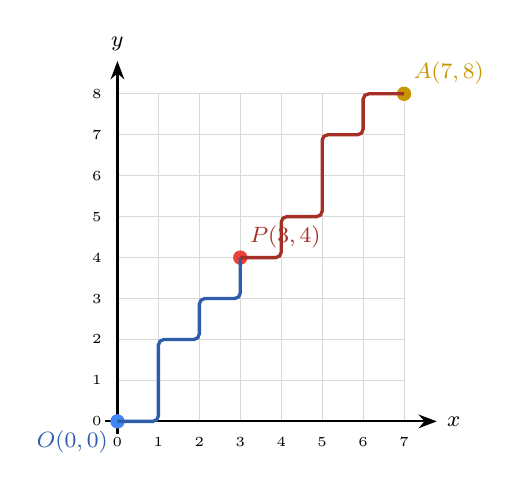
\begin{tikzpicture}[scale=0.52, >=Stealth, font=\small]
  % Grid
  \draw[gray!30] (0,0) grid (7,8);
  \draw[->, thick] (-0.3,0) -- (7.8,0) node[right, font=\footnotesize]{$x$};
  \draw[->, thick] (0,-0.3) -- (0,8.8) node[above, font=\footnotesize]{$y$};

  % Axis labels
  \foreach \x in {0,...,7}
    \node[below, font=\tiny] at (\x, -0.15) {$\x$};
  \foreach \y in {0,...,8}
    \node[left, font=\tiny] at (-0.15, \y) {$\y$};

  % Points
  \fill[setA] (0,0) circle (5pt);
  \node[below left, font=\footnotesize\bfseries, setA!70!black] at (0,0) {$O(0,0)$};

  \fill[setB] (3,4) circle (5pt);
  \node[above right, font=\footnotesize\bfseries, setB!70!black] at (3,4) {$P(3,4)$};

  \fill[setC!80!black] (7,8) circle (5pt);
  \node[above right, font=\footnotesize\bfseries, setC!80!black] at (7,8) {$A(7,8)$};

  % Sample path O -> P
  \draw[very thick, setA!70!black, rounded corners=2pt]
    (0,0) -- (1,0) -- (1,1) -- (1,2) -- (2,2) -- (2,3) -- (3,3) -- (3,4);

  % Sample path P -> A
  \draw[very thick, setB!70!black, rounded corners=2pt]
    (3,4) -- (4,4) -- (4,5) -- (5,5) -- (5,6) -- (5,7) -- (6,7) -- (6,8) -- (7,8);
\end{tikzpicture}
\end{center}
\end{theorybox}

\begin{problembox}
Գտեք $O(0,0)$ կետից $A(7,8)$ կետը տանող ցանցային ճանապարհների քանակը,
որոնք անցնում են $P(3,4)$ կետով։
\end{problembox}

\subsection*{Լուծում}

Ճանապարհը տրոհում ենք երկու անկախ հատվածի $P(3,4)$ կետում։

\textbf{Հատված 1: $O(0,0) \to P(3,4)$}\;
Պետք է 3 քայլ աջ և 4 քայլ վեր, ընդհանուր 7 քայլ։
Ընտրում ենք 3 աջ-քայլերը (կամ 4 վեր-քայլերը)․
\[
  \binom{3+4}{3} = \binom{7}{3}
  = \frac{7!}{3!\cdot 4!}
  = \frac{7 \cdot 6 \cdot 5}{3 \cdot 2 \cdot 1}
  = 35։
\]

\textbf{Հատված 2: $P(3,4) \to A(7,8)$}\;
$(3,4)$-ից $(7,8)$ հասնելու համար պետք է $7-3=4$ քայլ աջ և $8-4=4$ քայլ վեր,
ընդհանուր 8 քայլ։ Ընտրում ենք 4 աջ-քայլերը․
\[
  \binom{4+4}{4} = \binom{8}{4}
  = \frac{8!}{4!\cdot 4!}
  = \frac{8 \cdot 7 \cdot 6 \cdot 5}{4 \cdot 3 \cdot 2 \cdot 1}
  = 70։
\]

\textbf{Արտադրյալի կանոն.}\;
Երկու հատվածները անկախ են (առաջին հատվածի ցանկացած ճանապարհ կարող է
շարունակվել երկրորդ հատվածի ցանկացած ճանապարհով), ուստի․
\[
  \text{Ընդհանուր ճանապարհներ} = 35 \times 70 = 2450։
\]

\begin{answerbox}
\centering
$O(0,0)$-ից $A(7,8)$ տանող և $(3,4)$-ով անցնող ցանցային ճանապարհների
քանակն է $\binom{7}{3} \cdot \binom{8}{4} = 35 \cdot 70 = \boxed{2450}$։
\end{answerbox}

% ══════════════════════════════════════════════════════════════════
\newpage
\section{Խնդիր 9 — 6-ի տրոհումը երեք գումարելիների}
% ══════════════════════════════════════════════════════════════════

\begin{theorybox}[Աստղեր և գծիկներ / Թվի կոմպոզիցիաներ և տրոհումներ]
\textbf{Աստղեր և գծիկներ} (կրկնություններով զուգորդություններ).\;
\[
  x_1 + x_2 + \cdots + x_k = n, \qquad x_i \ge 0,
\]
հավասարման ոչ բացասական ամբողջական լուծումների քանակը
$\displaystyle\binom{n+k-1}{k-1}$ է։

\medskip
Եթե պահանջվում է $x_i \ge 1$ (դրական ամբողջ թվեր), տեղադրում ենք $y_i = x_i - 1 \ge 0$
և ստանում $y_1 + \cdots + y_k = n - k$, ինչը տալիս է
$\displaystyle\binom{n-1}{k-1}$ լուծում։

\medskip
\textbf{Թվի տրոհումներ (Integer partitions)} (չկարգավորված).\;
$n$ թվի տրոհումը $k$ մասերի դա $n$-ի ներկայացումն է
$n = \lambda_1 + \lambda_2 + \cdots + \lambda_k$ տեսքով, որտեղ
$\lambda_1 \ge \lambda_2 \ge \cdots \ge \lambda_k \ge 1$։
Կարգը էական չէ, այսինքն՝ $4+1+1$ և $1+4+1$ համարվում են \emph{նույն} տրոհումը։
\end{theorybox}

\begin{problembox}
Գտեք 6 թիվը երեք գումարելիների տրոհելու եղանակների քանակը։
\end{problembox}

\subsection*{Լուծում}

\textbf{Երկիմաստության նշում.}\; «Տրոհել երեք գումարելիների» կարող է նշանակել կարգավորված (կոմպոզիցիաներ) կամ չկարգավորված (բուն տրոհումներ)։ Մենք կլուծենք երկու տարբերակն էլ։

\subsubsection*{Տարբերակ 1: Կարգավորված գումարելիներ (կոմպոզիցիաներ)}

Փնտրում ենք հետևյալ հավասարման լուծումների քանակը․
\[
  x_1 + x_2 + x_3 = 6, \qquad x_i \ge 1.
\]
Ըստ աստղերի և գծիկների բանաձևի ($y_i = x_i - 1$ տեղադրմամբ)․
\[
  \binom{6-1}{3-1} = \binom{5}{2} = \frac{5!}{2!\cdot 3!} = 10.
\]

\begin{center}
\renewcommand{\arraystretch}{1.15}
\begin{tabular}{cccc}
\toprule
\textbf{\#} & $x_1$ & $x_2$ & $x_3$ \\
\midrule
1  & 4 & 1 & 1 \\
2  & 1 & 4 & 1 \\
3  & 1 & 1 & 4 \\
4  & 3 & 2 & 1 \\
5  & 3 & 1 & 2 \\
6  & 2 & 3 & 1 \\
7  & 1 & 3 & 2 \\
8  & 2 & 1 & 3 \\
9  & 1 & 2 & 3 \\
10 & 2 & 2 & 2 \\
\bottomrule
\end{tabular}
\end{center}

\subsubsection*{Տարբերակ 2: Չկարգավորված գումարելիներ (տրոհումներ)}

Փնտրում ենք $6 = \lambda_1 + \lambda_2 + \lambda_3$ ներկայացումների քանակը,
որտեղ $\lambda_1 \ge \lambda_2 \ge \lambda_3 \ge 1$։

Թվարկենք բոլոր հնարավորությունները․
\begin{center}
\renewcommand{\arraystretch}{1.15}
\begin{tabular}{cl}
\toprule
\textbf{\#} & \textbf{Տրոհում} \\
\midrule
1 & $4 + 1 + 1$ \\
2 & $3 + 2 + 1$ \\
3 & $2 + 2 + 2$ \\
\bottomrule
\end{tabular}
\end{center}

Կա ճիշտ \textbf{3} այդպիսի տրոհում։

\begin{answerbox}
\centering
\textbf{Կարգավորված} (կոմպոզիցիաներ դրական մասերով)՝
$\displaystyle\binom{5}{2} = 10$ եղանակ։\\[4pt]
\textbf{Չկարգավորված} (տրոհումներ 3 մասի)՝
$3$ եղանակ՝ \;$4{+}1{+}1$,\; $3{+}2{+}1$,\; $2{+}2{+}2$։
\end{answerbox}

% ══════════════════════════════════════════════════════════════════
\newpage
\section{Խնդիր 11 — «մաթեմատիկա» բառի վերադասավորումները}
% ══════════════════════════════════════════════════════════════════

\begin{theorybox}[Պոլինոմիալ գործակից / Տեղափոխություններ կրկնությամբ]
Եթե ունենք $n$ օբյեկտ, որտեղ կան $k$ տարբեր տեսակներ $n_1, n_2, \ldots, n_k$
քանակներով (այնպես որ $n_1 + n_2 + \cdots + n_k = n$), ապա տարբեր
դասավորությունների քանակը հավասար է \textbf{պոլինոմիալ գործակցին}․
\[
  \binom{n}{n_1,\, n_2,\, \ldots,\, n_k}
  = \frac{n!}{n_1!\cdot n_2!\cdots n_k!}։
\]

\medskip
\textbf{Իմաստը.}\;
Սկսում ենք $n!$ դասավորություններից (կարծես բոլոր տառերը տարբեր են),
ապա բաժանում ենք $n_i!$-ի յուրաքանչյուր նույնական տառի խմբի ներքին տեղափոխությունների համար։
\end{theorybox}

\begin{problembox}
Քանի՞ տարբեր բառ կարելի է կազմել՝ վերադասավորելով \textbf{«matematika»} բառի բոլոր տառերը։
\end{problembox}

\subsection*{Լուծում}

\textbf{Քայլ 1. Հաշվել տառերը և դրանց հաճախականությունները.}

«matematika» բառում կան հետևյալ տառերը․
\[
  \text{m -- a -- t -- e -- m -- a -- t -- i -- k -- a}
\]
Ընդհանուր $n = 10$ տառ։ Հաշվենք յուրաքանչյուրը․

\begin{center}
\renewcommand{\arraystretch}{1.2}
\begin{tabular}{lcccccc}
\toprule
\textbf{Տառ} & a & m & t & e & i & k \\
\midrule
\textbf{Քանակ} $n_i$ & 3 & 2 & 2 & 1 & 1 & 1 \\
\bottomrule
\end{tabular}
\end{center}

\textbf{Ստուգում.}\; $3 + 2 + 2 + 1 + 1 + 1 = 10$ \;\checkmark

\medskip
\textbf{Քայլ 2. Կիրառել պոլինոմիալ գործակիցը.}

\[
  \frac{10!}{3!\cdot 2!\cdot 2!\cdot 1!\cdot 1!\cdot 1!}
  = \frac{10!}{3!\cdot 2!\cdot 2!}
\]

Հաշվարկ․
\begin{align*}
  10! &= 3\,628\,800, \\
  3! \cdot 2! \cdot 2! &= 6 \cdot 2 \cdot 2 = 24, \\[4pt]
  \frac{3\,628\,800}{24} &= 151\,200.
\end{align*}

\begin{answerbox}
\centering
«matematika» բառի տարբեր վերադասավորումների քանակն է
$\displaystyle\frac{10!}{3!\cdot 2!\cdot 2!} = \boxed{151\,200}$։
\end{answerbox}

\end{document}
\newpage

% ── Practice 7 ───────────────────────────────────────────────────
\section{Գործնական 7 — Տրոհումներ}
\documentclass[12pt, a4paper]{article}

% ── Packages ──────────────────────────────────────────────────────
\usepackage{fontspec}
\setmainfont{Arial}
\usepackage{amsmath, amssymb, amsthm}
\usepackage{mathtools}
\usepackage{enumitem}
\usepackage{tikz}
\usetikzlibrary{calc, positioning, arrows.meta, fit, patterns, decorations.pathreplacing}
\usepackage{geometry}
\geometry{margin=2.4cm}
\usepackage{xcolor}
\usepackage{tcolorbox}
\tcbuselibrary{theorems, skins, breakable}
\usepackage{booktabs}
\usepackage{hyperref}
\hypersetup{colorlinks=true, linkcolor=blue!60!black, urlcolor=blue!60!black}

\setlength{\parindent}{0pt}
\setlength{\parskip}{6pt}

% ── Colours ───────────────────────────────────────────────────────
\definecolor{setA}{RGB}{66, 133, 244}   % blue
\definecolor{setB}{RGB}{234, 67, 53}    % red
\definecolor{setC}{RGB}{251, 188, 4}    % yellow
\definecolor{theoryBg}{RGB}{232, 245, 253}
\definecolor{theoryFrame}{RGB}{66, 133, 244}
\definecolor{stmtBg}{RGB}{255, 243, 224}
\definecolor{stmtFrame}{RGB}{230, 126, 34}
\definecolor{ansBg}{RGB}{232, 250, 232}
\definecolor{ansFrame}{RGB}{39, 174, 96}

% ── Environments ──────────────────────────────────────────────────
\newtcolorbox{theorybox}[1][]{%
  colback=theoryBg, colframe=theoryFrame,
  fonttitle=\bfseries, title={\small Տեսական Ակնարկ. #1},
  breakable, enhanced, arc=2mm,
  left=5pt, right=5pt, top=5pt, bottom=5pt
}

\newtcolorbox{problembox}{%
  colback=stmtBg, colframe=stmtFrame,
  fonttitle=\bfseries, title={\small Խնդրի Պահանջ},
  breakable, enhanced, arc=2mm,
  left=5pt, right=5pt, top=5pt, bottom=5pt
}

\newtcolorbox{answerbox}{%
  colback=ansBg, colframe=ansFrame,
  arc=2mm, left=5pt, right=5pt, top=3pt, bottom=3pt
}

\newcommand{\Z}{\mathbb{Z}}
\newcommand{\R}{\mathbb{R}}
\newcommand{\N}{\mathbb{N}}
\newcommand{\powset}[1]{2^{#1}}
\newcommand{\comp}[1]{\overline{#1}}
\newcommand{\symdiff}{\mathbin{\triangle}}

% ── Title ─────────────────────────────────────────────────────────
\title{\textbf{Գործնական 7 — Տրոհումներ և ներառման-բացառման սկզբունքը}\\[4pt]
       \large Ընտրված խնդիրների լուծումներ\\[2pt]
       \normalsize Խնդիրներ 1, 7, 10, 12}
\author{Դիսկրետ Մաթեմատիկա — ԵՊՀ}
\date{}

\begin{document}
\maketitle
\tableofcontents
\newpage

% ══════════════════════════════════════════════════════════════════
\section{Խնդիր 1 — 5-էլեմենտանի բազմության տրոհումը 3 դասերի}
% ══════════════════════════════════════════════════════════════════

\begin{theorybox}[Երկրորդ սեռի Ստիռլինգի թվեր]
\textbf{Երկրորդ սեռի Ստիռլինգի թիվը}՝ $S(n,k)$-ն, հաշվում է $n$-տարրանի բազմության տրոհումների քանակը ճիշտ $k$ հատ ոչ դատարկ, զույգ առ զույգ չհատվող ենթաբազմությունների (որոնք կոչվում են \emph{դասեր} կամ \emph{բլոկներ})։

\medskip
\textbf{Անդրադարձ առնչություն՝}
\[
  S(n,k) = S(n-1,\, k-1) \;+\; k \cdot S(n-1,\, k),
  \qquad n \ge 1,\; 1 \le k \le n։
\]

\textbf{Մեկնաբանություն՝}\; Դիտարկենք $n$-րդ տարրը։
\begin{itemize}[nosep]
  \item \emph{$n$-ը միայնակ է իր դասում՝}\;
        մնացած $n-1$ տարրերը կազմում են $k-1$ դասեր
        $\;\longrightarrow\; S(n-1,\,k-1)$ եղանակ։
  \item \emph{$n$-ը միանում է գոյություն ունեցող $k$ դասերից մեկին՝}\;
        նախ տրոհում ենք մնացած $n-1$ տարրերը $k$ դասերի
        ($S(n-1,\,k)$ եղանակ), ապա ընտրում ենք, թե որ դասին է միանում $n$-ը ($k$ ընտրություն)
        $\;\longrightarrow\; k \cdot S(n-1,\,k)$ եղանակ։
\end{itemize}

\medskip
\textbf{Եզրային պայմաններ՝}\;
$S(n,1) = 1$,\; $S(n,n) = 1$,\; $S(n,0) = 0$, երբ $n \ge 1$։

\begin{center}
\begin{tikzpicture}[scale=0.8, font=\small]
  % Set partition visual: {1,4}, {2,5}, {3}
  \node[font=\bfseries] at (-2, 1) {Օրինակ՝ $S(5,3)$};
  
  \node (n1) at (0,1.5) {1};
  \node (n4) at (1,1.5) {4};
  \node[draw=setA, thick, rounded corners, fit=(n1)(n4), inner sep=2pt, label={below:\tiny $\{1,4\}$}] {};
  
  \node (n2) at (2.5,1.5) {2};
  \node (n5) at (3.5,1.5) {5};
  \node[draw=setB, thick, rounded corners, fit=(n2)(n5), inner sep=2pt, label={below:\tiny $\{2,5\}$}] {};
  
  \node (n3) at (5,1.5) {3};
  \node[draw=setC!80!black, thick, rounded corners, fit=(n3), inner sep=2pt, label={below:\tiny $\{3\}$}] {};
  
  \node at (2.5, 0.5) {Տրոհում 3 բլոկի};
\end{tikzpicture}
\end{center}

\begin{center}
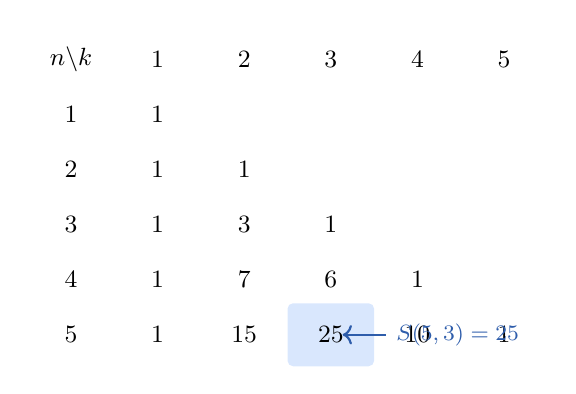
\begin{tikzpicture}[
  cell/.style={minimum width=1.1cm, minimum height=0.8cm, font=\small, anchor=center},
  header/.style={cell, font=\small\bfseries}
]
  % Header row
  \node[header] at (0, 0) {$n \backslash k$};
  \foreach \k [count=\i] in {1,2,3,4,5} {
    \node[header] at (\i*1.1, 0) {$\k$};
  }
  % Data rows
  \foreach \n/\vals [count=\row] in {
    1/{1},
    2/{1,1},
    3/{1,3,1},
    4/{1,7,6,1},
    5/{1,15,25,10,1}%
  } {
    \node[cell, font=\small\bfseries] at (0, -\row*0.7) {$\n$};
    \foreach \v [count=\col] in \vals {
      \ifnum\row=5
        \ifnum\col=3
          \node[cell, fill=setA!20, rounded corners=2pt] at (\col*1.1, -\row*0.7) {$\v$};
        \else
          \node[cell] at (\col*1.1, -\row*0.7) {$\v$};
        \fi
      \else
        \node[cell] at (\col*1.1, -\row*0.7) {$\v$};
      \fi
    }
  }
  % Highlight annotation
  \draw[->, thick, setA!70!black] (3.3+0.7, -3.5) -- (3.3+0.15, -3.5)
    node[right, pos=0, font=\footnotesize, setA!70!black] {$S(5,3)=25$};
\end{tikzpicture}
\end{center}
\end{theorybox}

\begin{problembox}
Քանի՞ եղանակով կարելի է $5$-տարրանի բազմությունը տրոհել $3$ ոչ դատարկ դասերի։
\end{problembox}

\subsection*{Լուծում}

Մեզ անհրաժեշտ է գտնել $S(5,3)$ Ստիռլինգի թիվը։ Օգտվելով անդրադարձ առնչությունից՝
\[
  S(5,3) = S(4,2) + 3 \cdot S(4,3)։
\]

\textbf{Հաշվում ենք $S(4,2)$-ը՝}
\[
  S(4,2) = S(3,1) + 2 \cdot S(3,2) = 1 + 2 \cdot 3 = 7։
\]

\textbf{Հաշվում ենք $S(4,3)$-ը՝}
\[
  S(4,3) = S(3,2) + 3 \cdot S(3,3) = 3 + 3 \cdot 1 = 6։
\]

\textbf{Վերջնական արդյունք՝}
\[
  S(5,3) = 7 + 3 \cdot 6 = 7 + 18 = 25։
\]

\textbf{Անկախ ստուգում։}\; Հաստատենք սա՝ դասակարգելով տրոհումները ըստ բլոկների չափերի (տրոհման կառուցվածք՝ $\{3,1,1\}$ և $\{2,2,1\}$)։

\textbf{Ստուգում բացահայտ թվարկմամբ։}\;
Դիցուք՝ բազմությունն է $\{a,b,c,d,e\}$։ 3 դասերի տրոհումը պետք է ունենա $\{3,1,1\}$ կամ $\{2,2,1\}$ կառուցվածքը (5-ի միակ տրոհումները 3 մասերի)։

\begin{itemize}[nosep]
  \item \textbf{Տիպ $\{3,1,1\}$՝}\;
        Ընտրում ենք 3-տարրանի բլոկը՝ $\binom{5}{3} = 10$ եղանակ։
        Մնացած 2 միատարր բազմությունները կազմում են չկարգավորված զույգ, որը տալիս է $1$ դասավորություն։
        Ընդամենը՝ $10$։
  \item \textbf{Տիպ $\{2,2,1\}$՝}\;
        Ընտրում ենք մեկ տարր պարունակող բլոկը՝ $\binom{5}{1} = 5$ եղանակ։
        Մնացած 4 տարրերը տրոհում ենք երկու զույգերի՝
        $\frac{1}{2!}\binom{4}{2} = 3$ եղանակ (բաժանում ենք $2!$-ի, քանի որ երկու զույգերը
        չկարգավորված են)։
        Ընդամենը՝ $5 \times 3 = 15$։
\end{itemize}

Ընդհանուր գումար՝ $10 + 15 = 25$։ \;\checkmark

\begin{answerbox}
\centering $S(5,3) = \boxed{25}$
\end{answerbox}

% ══════════════════════════════════════════════════════════════════
\newpage
\section{Խնդիր 7 — Բաժանելիությունը և Ներառման-բացառման սկզբունքը}
% ══════════════════════════════════════════════════════════════════

\begin{theorybox}[Ներառման-բացառման սկզբունք]
Վերջավոր բազմության (ունիվերսի) $A_1, A_2, \ldots, A_m$ ենթաբազմությունների համար՝
\[
  \biggl|\,\bigcup_{i=1}^{m} A_i\biggr|
  = \sum_{i} |A_i|
  - \sum_{i<j} |A_i \cap A_j|
  + \sum_{i<j<k} |A_i \cap A_j \cap A_k|
  - \cdots
\]

\begin{center}
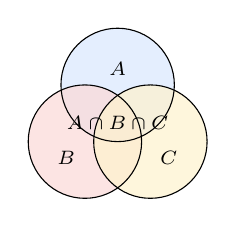
\begin{tikzpicture}[scale=0.6, font=\scriptsize]
  % 3-set Venn
  \coordinate (A) at (90:0.8);
  \coordinate (B) at (210:0.8);
  \coordinate (C) at (330:0.8);
  \fill[setA!20, opacity=0.7] (A) circle (1.2);
  \fill[setB!20, opacity=0.7] (B) circle (1.2);
  \fill[setC!20, opacity=0.7] (C) circle (1.2);
  \draw (A) circle (1.2) node[above] {$A$};
  \draw (B) circle (1.2) node[below left] {$B$};
  \draw (C) circle (1.2) node[below right] {$C$};
  \node at (0,0) {$A \cap B \cap C$};
\end{tikzpicture}
\end{center}

Հաշվելու համար այն տարրերը, որոնք չեն պատկանում $A_1, \ldots, A_m$ բազմություններից \textbf{ոչ մեկին}՝
\[
  \bigl|\comp{A_1} \cap \comp{A_2} \cap \cdots \cap \comp{A_m}\bigr|
  = |U| - \biggl|\,\bigcup_{i=1}^{m} A_i\biggr|։
\]

\medskip
\textbf{Կիրառությունը բաժանելիության խնդիրներում՝}\;
$\{1, 2, \ldots, N\}$ բազմության մեջ $d$-ի վրա բաժանվող ամբողջ թվերի քանակը
$\lfloor N/d \rfloor$ է։
Եթե $\gcd(d_1, d_2) = 1$, ապա միաժամանակ $d_1$-ի և $d_2$-ի վրա բաժանելիությունը համարժեք է $d_1 d_2$-ի վրա բաժանելիությանը։

\begin{center}
\begin{tikzpicture}[>=Stealth, font=\small, scale=0.85]
  \def\rr{1.6}
  \coordinate (cA) at (-0.65, 0);
  \coordinate (cB) at (0.65, 0);

  % Shade A only
  \begin{scope}
    \clip (cA) circle (\rr);
    \fill[setA!20] (-4,-4) rectangle (4,4);
  \end{scope}
  % Shade B only
  \begin{scope}
    \clip (cB) circle (\rr);
    \fill[setB!15] (-4,-4) rectangle (4,4);
  \end{scope}
  % Overlap
  \begin{scope}
    \clip (cA) circle (\rr);
    \clip (cB) circle (\rr);
    \fill[purple!20] (-4,-4) rectangle (4,4);
  \end{scope}

  \draw[thick, setA] (cA) circle (\rr);
  \draw[thick, setB] (cB) circle (\rr);

  \node[font=\footnotesize\bfseries, setA!70!black] at (-1.7, 1.1) {$A$};
  \node[font=\footnotesize\bfseries, setB!70!black] at (1.7, 1.1) {$B$};
Որոշում ենք ունիվերսալ բազմությունը (տիեզերքը) $S = 
  \node[font=\scriptsize] at (-1.4, 0.25) {$|A|-|A\!\cap\! B|$};
  \node[font=\scriptsize] at (0, -0.25) {$|A\!\cap\! B|$};
  \node[font=\scriptsize] at (1.4, 0.25) {$|B|-|A\!\cap\! B|$};

  \node[font=\footnotesize] at (0, -2.2) {$|A \cup B| = |A| + |B| - |A \cap B|$};
\end{tikzpicture}
\end{center}
\end{theorybox}

\begin{problembox}
$1$-ից $16500$ միջակայքում քանի՞ ամբողջ թիվ կա, որ չի բաժանվում $5$-ի, չի բաժանվում $3$-ի, բայց \textbf{բաժանվում է} $11$-ի վրա։
\end{problembox}

\subsection*{Լուծում}

\textbf{Քայլ 0. Ընտրում ենք ունիվերսը։}\; Ներառման-բացառման ցանկացած խնդրում առաջին քայլը \emph{ունիվերսի ընտրությունն է}։ Այստեղ մենք որպես $S$ վերցնում ենք $\{1, \ldots, 16500\}$ միջակայքի այն թվերը, որոնք բաժանվում են 11-ի։ Բոլոր հաշվարկները կատարվում են $S$-ի ներսում։

\medskip
Դիցուք $S$-ը $\{1, 2, \ldots, 16500\}$ հատվածի այն ամբողջ թվերի բազմությունն է, որոնք բաժանվում են $11$-ի։ Մենք ցանկանում ենք $S$-ից հեռացնել այն թվերը, որոնք բաժանվում են նաև $3$-ի կամ $5$-ի։

Սահմանենք՝
\begin{align*}
  A &= \{n \in S \mid 3 \mid n\}
      &&\text{(բաժանվում է և՛ 11-ի, և՛ 3-ի, այսինքն՝ 33-ի)}, \\
  B &= \{n \in S \mid 5 \mid n\}
      &&\text{(բաժանվում է և՛ 11-ի, և՛ 5-ի, այսինքն՝ 55-ի)}։
\end{align*}

Մենք փնտրում ենք $|S| - |A \cup B|$ արժեքը։

\textbf{Քայլ 1. Հաշվում ենք առանձին քանակները։}
\[
\renewcommand{\arraystretch}{1.3}
\begin{array}{rclcl}
  |S| &=& \lfloor 16500/11 \rfloor &=& 1500, \\
  |A| &=& \lfloor 16500/33 \rfloor &=& 500, \\
  |B| &=& \lfloor 16500/55 \rfloor &=& 300, \\
  |A \cap B| &=& \lfloor 16500/165 \rfloor &=& 100։
\end{array}
\]
Այստեղ $|A \cap B|$-ն հաշվում է $\text{lcm}(33,55) = 165$-ի վրա բաժանվող թվերը։

\textbf{Քայլ 2. Կիրառում ենք ներառման-բացառման սկզբունքը։}
\[
  |A \cup B| = |A| + |B| - |A \cap B| = 500 + 300 - 100 = 700։
\]

\textbf{Քայլ 3. Հանում ենք։}
\[
  |S \setminus (A \cup B)| = |S| - |A \cup B| = 1500 - 700 = 800։
\]

\begin{center}
\begin{tikzpicture}[>=Stealth, font=\small, scale=0.9]
  % Universe = S (div by 11)
  \draw[thick, gray, rounded corners=8pt, fill=gray!5]
    (-3.2, -2.0) rectangle (3.2, 2.2);
  \node[gray, font=\footnotesize\bfseries] at (2.5, 1.9) {$S\;(1500)$};

  \def\rr{1.2}
  \coordinate (cA) at (-0.5, 0);
  \coordinate (cB) at (0.5, 0);

  \fill[setA!20] (cA) circle (\rr);
  \fill[setB!15] (cB) circle (\rr);
  \begin{scope}
    \clip (cA) circle (\rr);
    \fill[purple!25] (cB) circle (\rr);
  \end{scope}

  \draw[thick, setA] (cA) circle (\rr);
  \draw[thick, setB] (cB) circle (\rr);

  \node[font=\footnotesize\bfseries, setA!70!black] at (-1.6, 0.8) {$A$};
  \node[font=\footnotesize\bfseries, setB!70!black] at (1.6, 0.8) {$B$};

  \node[font=\scriptsize] at (-1.1, 0) {$400$};
  \node[font=\scriptsize] at (0, 0) {$100$};
  \node[font=\scriptsize] at (1.1, 0) {$200$};

  \node[font=\footnotesize, ansFrame!80!black] at (-2.4, -1.3) {\textbf{800}};
  \draw[->, thick, ansFrame!70!black] (-2.4, -1.1) -- (-2.4, -0.2);
  \node[font=\scriptsize, gray] at (-2.4, -1.6) {պատ․};
\end{tikzpicture}
\end{center}

\begin{answerbox}
\centering $\boxed{800}$ թիվ 1-ից 16500 միջակայքում բաժանվում է 11-ի,
բայց ոչ 3-ի և ոչ էլ 5-ի։
\end{answerbox}

% ══════════════════════════════════════════════════════════════════
\newpage
\section{Խնդիր 10 — Եռանկյուններ եռանկյունաձև ցանցում}
% ══════════════════════════════════════════════════════════════════

\begin{theorybox}[Եռանկյունների հաշվումը եռանկյունաձև ցանցում]
Երբ հավասարակողմ եռանկյան յուրաքանչյուր կողմ բաժանվում է $n$ հավասար հատվածների, և բաժանման կետերը միացվում են կողմերին զուգահեռ գծերով, առաջանում է $n$ կողմով \textbf{եռանկյունաձև ցանց}։

\medskip
Ցանցը պարունակում է երկու տիպի եռանկյուններ, որոնց կողմերը զուգահեռ են սկզբնական եռանկյան կողմերին՝

\begin{enumerate}[nosep]
  \item \textbf{Դեպի վեր ուղղված} ($s$ կողմով, $1 \le s \le n$)՝
        $U(n,s) = \binom{n-s+2}{2}$։
  \item \textbf{Դեպի վար ուղղված} ($s$ կողմով, $1 \le s \le \lfloor n/2 \rfloor$)՝
        $D(n,s) = \binom{n-2s+2}{2}$։
\end{enumerate}

\begin{center}
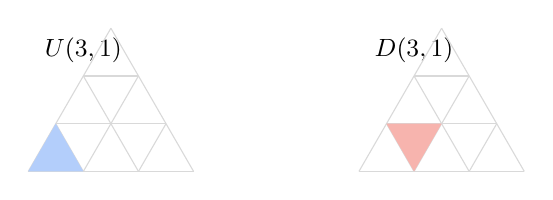
\begin{tikzpicture}[scale=0.7, font=\small]
  % Visual explosion of U/D
  % Base U triangle
  \begin{scope}[xshift=-3cm]
    \node[anchor=south] at (1, 1.8) {$U(3,1)$};
    \foreach \i in {0,...,3} \draw[gray!30] (\i/2, {\i*sqrt(3)/2}) -- (3 - \i/2, {\i*sqrt(3)/2});
    \foreach \i in {0,...,3} \draw[gray!30] (\i, 0) -- (\i/2, {\i*sqrt(3)/2});
    \foreach \i in {0,...,3} \draw[gray!30] (\i, 0) -- ({(3+\i)/2}, {(3-\i)*sqrt(3)/2});
    \fill[setA!40] (0,0) -- (1,0) -- (0.5,{sqrt(3)/2}) -- cycle;
  \end{scope}

  % Base D triangle
  \begin{scope}[xshift=3cm]
    \node[anchor=south] at (1, 1.8) {$D(3,1)$};
    \foreach \i in {0,...,3} \draw[gray!30] (\i/2, {\i*sqrt(3)/2}) -- (3 - \i/2, {\i*sqrt(3)/2});
    \foreach \i in {0,...,3} \draw[gray!30] (\i, 0) -- (\i/2, {\i*sqrt(3)/2});
    \foreach \i in {0,...,3} \draw[gray!30] (\i, 0) -- ({(3+\i)/2}, {(3-\i)*sqrt(3)/2});
    \fill[setB!40] (0.5,{sqrt(3)/2}) -- (1.5,{sqrt(3)/2}) -- (1,0) -- cycle;
  \end{scope}
\end{tikzpicture}
\end{center}

\begin{center}
\begin{tikzpicture}[scale=0.7, font=\small]
  % Small grid n=4 for illustration
  \def\n{4}
  % Draw grid lines
  \foreach \i in {0,...,\n} {
    % horizontal-ish lines (parallel to base)
    \draw[gray!50] (\i/2, {\i*sqrt(3)/2}) -- (\n - \i/2, {\i*sqrt(3)/2});
    % left-leaning lines
    \draw[gray!50] (\i, 0) -- (\i/2, {\i*sqrt(3)/2});
    % right-leaning lines
    \draw[gray!50] (\i, 0) -- ({(\n+\i)/2}, {(\n-\i)*sqrt(3)/2});
  }
  % Outer triangle
  \draw[thick] (0,0) -- (\n, 0) -- (\n/2, {\n*sqrt(3)/2}) -- cycle;

  % Highlight an upward triangle of side 2 (blue)
  \fill[setA!25, opacity=0.6] (0,0) -- (2,0) -- (1, {sqrt(3)}) -- cycle;
  \draw[thick, setA] (0,0) -- (2,0) -- (1, {sqrt(3)}) -- cycle;
  \node[font=\scriptsize, setA!70!black] at (1, 0.5) {$s\!=\!2$};

  % Highlight a downward triangle of side 1 (red)
  \fill[setB!25, opacity=0.6] (1.5, {sqrt(3)/2}) -- (2, 0) -- (2.5, {sqrt(3)/2}) -- cycle;
  \draw[thick, setB] (1.5, {sqrt(3)/2}) -- (2, 0) -- (2.5, {sqrt(3)/2}) -- cycle;

  % Labels
  \node[font=\footnotesize] at (2, -0.9) {Ցանց $n=4$-ով};
  \node[font=\scriptsize, setA!70!black] at (-1.8, 1.5) {դեպի վեր};
  \draw[->, setA!70!black, thin] (-1.0, 1.35) -- (0.4, 0.8);
  \node[font=\scriptsize, setB!70!black] at (4.6, 1.5) {դեպի վար};
  \draw[->, setB!70!black, thin] (4.0, 1.3) -- (2.3, 0.45);
\end{tikzpicture}
\end{center}
\end{theorybox}

\begin{problembox}
$ABC$ եռանկյան յուրաքանչյուր կողմը բաժանված է $8$ հավասար հատվածների։
Բաժանման կետերով անցնող և կողմերին զուգահեռ տարված ուղիղները կազմում են եռանկյունաձև ցանց։
Քանի՞ եռանկյուն կարելի է կազմել այս ցանցի կետերով, որոնց կողմերը զուգահեռ են $ABC$-ի կողմերին։
\end{problembox}

\subsection*{Լուծում}

Ունենք եռանկյունաձև ցանց $n = 8$ պարամետրով։ Մենք հաշվում ենք դեպի վեր և դեպի վար ուղղված եռանկյունները առանձին։

\textbf{Ի՞նչ ենք հաշվում։}\; «$s$ կողմով դեպի վեր եռանկյունը» այն եռանկյունն է, որն ունի նույն կողմնորոշումը, ինչ արտաքին եռանկյունը, և որի կողմը ընդգրկում է $s$ ցանցային միավոր։ «$s$ կողմով դեպի վար եռանկյունը» շրջված է։ Երկու տիպերն էլ պետք է ունենան արտաքին եռանկյանը զուգահեռ կողմեր։

\textbf{$s$ կողմով դեպի վեր եռանկյուններ ($1 \le s \le 8$)՝}
\[
  U(8,s) = \frac{(8-s+1)(8-s+2)}{2} = \binom{10-s}{2}։
\]

\begin{center}
\renewcommand{\arraystretch}{1.3}
\begin{tabular}{c|cccccccc|c}
\toprule
$s$ & 1 & 2 & 3 & 4 & 5 & 6 & 7 & 8 & Գումար \\
\midrule
$U(8,s)$ & 36 & 28 & 21 & 15 & 10 & 6 & 3 & 1 & \textbf{120} \\
\bottomrule
\end{tabular}
\end{center}

\[
  \sum_{s=1}^{8} U(8,s) = 36 + 28 + 21 + 15 + 10 + 6 + 3 + 1 = 120.
\]

\textbf{$s$ կողմով դեպի վար եռանկյուններ
($1 \le s \le \lfloor 8/2 \rfloor = 4$)՝}
\[
  D(8,s) = \frac{(8-2s+1)(8-2s+2)}{2} = \binom{10-2s}{2}։
\]

\begin{center}
\renewcommand{\arraystretch}{1.3}
\begin{tabular}{c|cccc|c}
\toprule
$s$ & 1 & 2 & 3 & 4 & Գումար \\
\midrule
$D(8,s)$ & 28 & 15 & 6 & 1 & \textbf{50} \\
\bottomrule
\end{tabular}
\end{center}

\[
  \sum_{s=1}^{4} D(8,s) = 28 + 15 + 6 + 1 = 50.
\]

\textbf{Ընդհանուր գումար՝}
\[
  120 + 50 = 170։
\]

\begin{center}
\begin{tikzpicture}[scale=0.38, font=\small]
  % Draw the n=8 grid
  \def\n{8}
  \foreach \i in {0,...,\n} {
    \draw[gray!40] (\i/2, {\i*sqrt(3)/2}) -- (\n - \i/2, {\i*sqrt(3)/2});
    \draw[gray!40] (\i, 0) -- (\i/2, {\i*sqrt(3)/2});
    \draw[gray!40] (\i, 0) -- ({(\n+\i)/2}, {(\n-\i)*sqrt(3)/2});
  }
  \draw[very thick] (0,0) -- (\n, 0) -- (\n/2, {\n*sqrt(3)/2}) -- cycle;

  % Example upward triangle of side 3 (blue)
  \fill[setA!20, opacity=0.5] (0.5, {sqrt(3)/2}) -- (3.5, {sqrt(3)/2})
    -- (2, {4*sqrt(3)/2}) -- cycle;
  \draw[thick, setA] (0.5, {sqrt(3)/2}) -- (3.5, {sqrt(3)/2})
    -- (2, {4*sqrt(3)/2}) -- cycle;

  % Example downward triangle of side 2 (red)
  \fill[setB!20, opacity=0.5] (3, {2*sqrt(3)/2}) -- (5, {2*sqrt(3)/2})
    -- (4, {0*sqrt(3)/2+0}) -- cycle;
  \draw[thick, setB] (3, {2*sqrt(3)/2}) -- (5, {2*sqrt(3)/2})
    -- (4, 0) -- cycle;

  \node[font=\footnotesize\bfseries] at (4, -1.2) {Ցանց $n = 8$-ով};
\end{tikzpicture}
\end{center}

\begin{answerbox}
\centering $ABC$-ի կողմերին զուգահեռ եռանկյունների ընդհանուր քանակը
$\boxed{170}$ է\; (120 դեպի վեր $+$ 50 դեպի վար)։
\end{answerbox}

% ══════════════════════════════════════════════════════════════════
\newpage
\section{Խնդիր 12 — Սահմանափակմամբ ամբողջ լուծումներ}
% ══════════════════════════════════════════════════════════════════

\begin{theorybox}[Ամբողջ լուծումների հաշվումը վերին սահմաններով]
$y_1 + y_2 + \cdots + y_r = n$ հավասարման ոչ բացասական ամբողջ լուծումները հաշվելու համար՝ $y_i \le u_i$ սահմանափակումներով.

\begin{enumerate}[nosep]
  \item \textbf{Առանց վերին սահմանների՝}\;
        Լուծումների քանակը $\binom{n+r-1}{r-1}$ է («աստղերի և գծիկների» մեթոդ)։
  \item \textbf{Հանում ենք խախտումները}՝ օգտագործելով ներառման-բացառման սկզբունքը։
        Դիցուք $A_i$-ն այն լուծումների բազմությունն է, որտեղ $y_i > u_i$։
        Տեղադրելով $z_i = y_i - (u_i + 1) \ge 0$՝ $|A_i|$ քանակը
        դառնում է առանց սահմանափակման խնդիր՝ նվազեցված գումարով։
  \item \textbf{Հատումներ՝}\;
        $|A_i \cap A_j|$-ի համար տեղադրում ենք և՛ $z_i = y_i - (u_i+1)$,
        և՛ $z_j = y_j - (u_j+1)$։
        Եթե մնացած գումարը բացասական է, ապա լուծումների քանակը $0$ է։
\end{enumerate}

\medskip
\textbf{Բանաձև՝}
\[
  \text{պատասխան} = \sum_{S \subseteq \{1,\ldots,r\}} (-1)^{|S|}
  \binom{n - \sum_{i \in S}(u_i+1) + r - 1}{r-1},
\]
որտեղ բինոմիալ գործակցի բացասական վերին անդամով դեպքերը հավասար են $0$-ի։
\end{theorybox}

\begin{problembox}
Գտնել ամբողջ լուծումների քանակը հետևյալ համակարգի համար՝
\[
  x_1 + x_2 + x_3 = 40, \qquad
  4 \le x_1 \le 15, \quad
  9 \le x_2 \le 18, \quad
  5 \le x_3 \le 16։
\]
\end{problembox}

\subsection*{Լուծում}

\textbf{Քայլ 1. Փոփոխականների տեղաշարժ ստորին սահմանները հեռացնելու համար։}

Նշանակենք $y_1 = x_1 - 4$,\; $y_2 = x_2 - 9$,\; $y_3 = x_3 - 5$։
Այդ դեպքում՝
\[, \quad
        z_1 + y_2 + y_3 = 10\text{։}
  &\quad |A_1| &= \binom{12}{2} = 66\text{։} \\
  A_2 &:\; y_2 \ge 10. \quad
        \text{Տեղադրենք } z_2 = y_2 - 10 \ge 0, \quad
        y_1 + z_2 + y_3 = 12\text{։}
  &\quad |A_2| &= \binom{14}{2} = 91\text{։} \\
  A_3 &:\; y_3 \ge 12. \quad
        \text{Տեղադրենք } z_3 = y_3 - 12 \ge 0, \quad
        y_1 + y_2 + z_3 = 10\text{։}
  &\quad |A_3| &= \binom{12}{2} = 66\text{։}

\textbf{Քայլ 3. Սահմանում ենք խախտման բազմությունները և կիրառում ներառման-բացառման սկզբունքը։}

Դիցուք $A_i$-ն այն լուծումների բազմությունն է, որտեղ $y_i$-ն գերազանցում է իր վերին սահմանը.
\begin{align*}
  A_1 &:\; y_1 \ge 12. \quad
        \text{Տեղադրենք } z_1 = y_1 - 12 \ge 0;\;
        z_1 + y_2 + y_3 = 10.
  &\quad |A_1| &= \binom{12}{2} = 66. \\
  A_2 &:\; y_2 \ge 10. \quad
        \text{Տեղադրենք } z_2 = y_2 - 10 \ge 0;\;
        y_1 + z_2 + y_3 = 12.
  &\quad |A_2| &= \binom{14}{2} = 91. \\
  A_3 &:\; y_3 \ge 12. \quad
        \text{Տեղադրենք } z_3 = y_3 - 12 \ge 0;\;
        y_1 + y_2 + z_3 = 10.
  &\quad |A_3| &= \binom{12}{2} = 66:
\end{align*}

\textbf{Քայլ 4. Զույգ առ զույգ հատումներ։}

$A_1 \cap A_2$: $y_1 \ge 12,\; y_2 \ge 10$.
Մնացած գումարը՝ $22 - 12 - 10 = 0$։
\quad $|A_1 \cap A_2| = \binom{2}{2} = 1$։

$A_1 \cap A_3$: $y_1 \ge 12,\; y_3 \ge 12$.
Մնացած գումարը՝ $22 - 12 - 12 = -2 < 0$։
\quad $|A_1 \cap A_3| = 0$։
Բացասական մնացորդային գումարը նշանակում է, որ համակարգը անհնարին է. ոչ բացասական փոփոխականների գումարը չի կարող լինել բացասական, ուստի լուծումների քանակը $0$ է։

$A_2 \cap A_3$: $y_2 \ge 10,\; y_3 \ge 12$.
Մնացած գումարը՝ $22 - 10 - 12 = 0$։
\quad $|A_2 \cap A_3| = \binom{2}{2} = 1$։

\textbf{Քայլ 5. Եռակի հատում։}
\[
  A_1 \cap A_2 \cap A_3:\; y_1 \ge 12,\; y_2 \ge 10,\; y_3 \ge 12.
  \quad \text{Գումարը } \ge 34 > 22։ \quad |A_1 \cap A_2 \cap A_3| = 0։
\]

\textbf{Քայլ 6. Միավորում՝ ըստ ներառման-բացառման սկզբունքի։}
\begin{align*}
  |A_1 \cup A_2 \cup A_3|
  &= (66 + 91 + 66) - (1 + 0 + 1) + 0 \\
  &= 223 - 2 = 221։
\end{align*}

\textbf{Վերջնական հաշվարկ՝}
\[
  276 - 221 = 55։
\]

\begin{center}
\begin{tikzpicture}[>=Stealth, font=\small, scale=0.85]
  \def\rr{1.3}
  \coordinate (cA) at (90:0.55);
  \coordinate (cB) at (210:0.55);
  \coordinate (cC) at (330:0.55);

  \fill[setA!15] (cA) circle (\rr);
  \fill[setB!12] (cB) circle (\rr);
  \fill[setC!12] (cC) circle (\rr);

  % Pairwise overlaps
  \begin{scope}
    \clip (cA) circle (\rr);
    \fill[purple!20] (cB) circle (\rr);
  \end{scope}
  \begin{scope}
    \clip (cB) circle (\rr);
    \fill[orange!20] (cC) circle (\rr);
  \end{scope}

  \draw[thick, setA] (cA) circle (\rr);
  \draw[thick, setB] (cB) circle (\rr);
  \draw[thick, setC] (cC) circle (\rr);

  \node[font=\footnotesize\bfseries, setA!70!black] at (90:2.1) {$A_1\;(66)$};
  \node[font=\footnotesize\bfseries, setB!70!black] at (210:2.1) {$A_2\;(91)$};
  \node[font=\footnotesize\bfseries, setC!80!black] at (330:2.1) {$A_3\;(66)$};

  \node[font=\tiny] at (150:0.85) {$1$};
  \node[font=\tiny, gray] at (30:0.85) {$0$};
  \node[font=\tiny] at (270:0.85) {$1$};
  \node[font=\tiny, gray] at (0:0) {$0$};

  \node[font=\footnotesize] at (0, -2.5)
    {$|A_1 \cup A_2 \cup A_3| = 221$};
  \node[font=\footnotesize\bfseries, ansFrame!80!black] at (0, -3.2)
    {Պատասխան՝ $276 - 221 = 55$};
\end{tikzpicture}
\end{center}

\begin{answerbox}
\centering Ամբողջ լուծումների քանակն է՝ $\boxed{55}$։
\end{answerbox}

\end{document}
\newpage

% ── Practice 8 ───────────────────────────────────────────────────
\section{Գործնական 8 — Անդրադարձ առնչություններ}
\documentclass[12pt, a4paper]{article}

% ── Packages ──────────────────────────────────────────────────────
\usepackage{fontspec}
\setmainfont{Arial}
\usepackage{amsmath, amssymb, amsthm}
\usepackage{mathtools}
\usepackage{enumitem}
\usepackage{tikz}
\usetikzlibrary{calc, positioning, arrows.meta, fit, patterns, decorations.pathreplacing}
\usepackage{geometry}
\geometry{margin=2.4cm}
\usepackage{xcolor}
\usepackage{tcolorbox}
\tcbuselibrary{theorems, skins, breakable}
\usepackage{booktabs}
\usepackage{hyperref}
\hypersetup{colorlinks=true, linkcolor=blue!60!black, urlcolor=blue!60!black}

\setlength{\parindent}{0pt}
\setlength{\parskip}{6pt}

% ── Colours ───────────────────────────────────────────────────────
\definecolor{setA}{RGB}{66, 133, 244}   % blue
\definecolor{setB}{RGB}{234, 67, 53}    % red
\definecolor{setC}{RGB}{251, 188, 4}    % yellow
\definecolor{theoryBg}{RGB}{232, 245, 253}
\definecolor{theoryFrame}{RGB}{66, 133, 244}
\definecolor{stmtBg}{RGB}{255, 243, 224}
\definecolor{stmtFrame}{RGB}{230, 126, 34}
\definecolor{ansBg}{RGB}{232, 250, 232}
\definecolor{ansFrame}{RGB}{39, 174, 96}

% ── Environments ──────────────────────────────────────────────────
\newtcolorbox{theorybox}[1][]{%
  colback=theoryBg, colframe=theoryFrame,
  fonttitle=\bfseries, title={\small Տեսության ամփոփում. #1},
  breakable, enhanced, arc=2mm,
  left=5pt, right=5pt, top=5pt, bottom=5pt
}

\newtcolorbox{problembox}{%
  colback=stmtBg, colframe=stmtFrame,
  fonttitle=\bfseries, title={\small Խնդրի դրվածք},
  breakable, enhanced, arc=2mm,
  left=5pt, right=5pt, top=5pt, bottom=5pt
}

\newtcolorbox{answerbox}{%
  colback=ansBg, colframe=ansFrame,
  arc=2mm, left=5pt, right=5pt, top=3pt, bottom=3pt
}

\newcommand{\Z}{\mathbb{Z}}
\newcommand{\R}{\mathbb{R}}
\newcommand{\N}{\mathbb{N}}
\newcommand{\powset}[1]{2^{#1}}
\newcommand{\comp}[1]{\overline{#1}}
\newcommand{\symdiff}{\mathbin{\triangle}}

% ── Title ─────────────────────────────────────────────────────────
\title{\textbf{Գործնական 8 — Անդրադարձ առնչություններ}\\[4pt]
       \large Ընտրված խնդիրների լուծումներ\\[2pt]
       \normalsize Խնդիրներ 2, 6}
\author{Դիսկրետ Մաթեմատիկա — ԵՊՀ}
\date{}

\begin{document}
\maketitle
\tableofcontents
\newpage

% ══════════════════════════════════════════════════════════════════
\section{Խնդիր 2 — Երկրորդ կարգի գծային անդրադարձ առնչության լուծում}
% ══════════════════════════════════════════════════════════════════

\begin{theorybox}[Հաստատուն գործակիցներով երկրորդ կարգի գծային անդրադարձ առնչություններ]
\textbf{Հաստատուն գործակիցներով երկրորդ կարգի գծային անդրադարձ առնչությունն} ունի հետևյալ տեսքը՝
\[
  a_n = c_1\, a_{n-1} + c_2\, a_{n-2}, \qquad n \ge 2,
\]
որտեղ $c_1, c_2$ հաստատուններ են, իսկ $a_0, a_1$ (կամ $a_1, a_2$) տրված սկզբնական արժեքներն են։

\medskip
\textbf{Բնութագրիչ հավասարման մեթոդ։}\;
Առնչության մեջ տեղադրելով $a_n = r^n$ փորձնական լուծումը՝ կստանանք \textbf{բնութագրիչ հավասարումը}։
\[
  r^2 - c_1\, r - c_2 = 0.
\]

Ընդհանուր լուծման տեսքը կախված է $r_1, r_2$ արմատներից։

\medskip
\begin{center}
\renewcommand{\arraystretch}{1.5}
\begin{tabular}{lll}
\toprule
\textbf{Դեպք} & \textbf{Արմատներ} & \textbf{Ընդհանուր Լուծում} \\
\midrule
Տարբեր իրական արմատներ & $r_1 \neq r_2$, երկուսն էլ իրական
  & $a_n = \alpha\, r_1^n + \beta\, r_2^n$ \\
Պատիկ իրական արմատներ & $r_1 = r_2 = r$
  & $a_n = (\alpha + \beta\, n)\, r^n$ \\
Կոմպլեքս համալուծ արմատներ & $r_{1,2} = \rho\, e^{\pm i\theta}$
  & $a_n = \rho^n\bigl(\alpha \cos n\theta + \beta \sin n\theta\bigr)$ \\
\bottomrule
\end{tabular}
\end{center}

\medskip
$\alpha$ և $\beta$ հաստատունները որոշվում են ընդհանուր լուծման մեջ սկզբնական պայմանները տեղադրելու և ստացված $2 \times 2$ գծային հավասարումների համակարգը լուծելու միջոցով։

\begin{center}
\begin{tikzpicture}[>=Stealth, font=\small, node distance=1.6cm]
  \node[draw, rounded corners=4pt, fill=stmtBg, minimum width=2.8cm,
        align=center, font=\small] (rec) {Առնչություն\\$a_n = c_1 a_{n-1} + c_2 a_{n-2}$};
  \node[draw, rounded corners=4pt, fill=theoryBg, minimum width=2.8cm,
        align=center, font=\small, right=2.6cm of rec] (char)
    {Բնութագրիչ հավ.\\$r^2 - c_1 r - c_2 = 0$};
  \node[draw, rounded corners=4pt, fill=setC!15, minimum width=2.8cm,
        align=center, font=\small, right=2.6cm of char] (gen)
    {Ընդհանուր լուծում\\$a_n = \alpha r_1^n + \beta r_2^n$};
  \node[draw, rounded corners=4pt, fill=ansBg, minimum width=2.8cm,
        align=center, font=\small, below=1.4cm of gen] (sol)
    {Մասնավոր լուծում\\(սկզբն. պայմաններ)};

  \draw[->, thick] (rec) -- (char)
    node[midway, above=3pt, font=\scriptsize]{տեղադրել $a_n = r^n$};
  \draw[->, thick] (char) -- (gen)
    node[midway, above=3pt, font=\scriptsize]{գտնել արմատները};
  \draw[->, thick] (gen) -- (sol)
    node[midway, right=3pt, font=\scriptsize]{գտնել $\alpha, \beta$};
\end{tikzpicture}
\end{center}
\end{theorybox}

\begin{problembox}
Լուծել գծային անդրադարձ առնչությունը.
\[
  a_n = 5a_{n-1} - 6a_{n-2}, \qquad n \ge 3,
\]
տրված $a_1 = 2$ և $a_2 = 10$ սկզբնական պայմաններով։
\end{problembox}

\subsection*{Լուծում}

\textbf{Ո՞ր դեպքն է։}\; Բնութագրիչ հավասարման արմատները գտնելուց հետո ընտրում ենք ընդհանուր լուծման ձևը։
\begin{itemize}[nosep]
  \item Տարբեր իրական արմատներ $r_1 \neq r_2$. $a_n = \alpha\, r_1^n + \beta\, r_2^n$։
  \item Պատիկ իրական արմատներ $r_1 = r_2 = r$. $a_n = (\alpha + \beta\, n)\, r^n$։
  \item Կոմպլեքս համալուծ արմատներ $\rho\, e^{\pm i\theta}$. $a_n = \rho^n(\alpha \cos n\theta + \beta \sin n\theta)$։
\end{itemize}

\medskip
\textbf{Քայլ 1. Գրել բնութագրիչ հավասարումը։}

$a_n - 5a_{n-1} + 6a_{n-2} = 0$ առնչության բնութագրիչ հավասարումն է՝
\[
  r^2 - 5r + 6 = 0.
\]

\textbf{Քայլ 2. Գտնել արմատները։}

Վերլուծելով արտադրիչների՝
\[
  r^2 - 5r + 6 = (r - 2)(r - 3) = 0
  \qquad\Longrightarrow\qquad r_1 = 2, \quad r_2 = 3.
\]
Քանի որ արմատներն իրական են և իրարից տարբեր, մենք գործ ունենք \textbf{առաջին դեպքի} հետ։

\begin{center}
\begin{tikzpicture}[>=Stealth, font=\small]
  % Parabola for r^2 - 5r + 6
  \draw[->, thick] (-0.5, 0) -- (5.5, 0) node[right]{$r$};
  \draw[->, thick] (0, -1.5) -- (0, 4) node[above]{$r^2 - 5r + 6$};

  \draw[thick, setA, domain=0.5:4.5, samples=60]
    plot (\x, {(\x - 2)*(\x - 3)});

  % Roots
  \fill[setB] (2, 0) circle (3pt) node[below left=3pt, font=\footnotesize]{$r_1 = 2$};
  \fill[setB] (3, 0) circle (3pt) node[below right=3pt, font=\footnotesize]{$r_2 = 3$};

  % Tick marks
  \foreach \x in {1, 2, 3, 4} {
    \draw (\x, 0.08) -- (\x, -0.08);
  }
  \node[below, font=\tiny] at (1, -0.08) {$1$};
  \node[below, font=\tiny] at (4, -0.08) {$4$};
\end{tikzpicture}
\end{center}

\textbf{Քայլ 3. Գրել ընդհանուր լուծումը։}

Քանի որ $r_1 = 2$ և $r_2 = 3$ տարբեր իրական արմատներ են՝
\[
  a_n = \alpha \cdot 2^n + \beta \cdot 3^n.
\]

\textbf{Քայլ 4. Կիրառել սկզբնական պայմանները։}

Տեղադրելով $n = 1$ և $n = 2$՝
\[
  \begin{cases}
    a_1 = 2\alpha + 3\beta = 2 \\[3pt]
    a_2 = 4\alpha + 9\beta = 10
  \end{cases}
\]

\textbf{Նշում.}\; Սա $2 \times 2$ գծային հավասարումների համակարգ է։

Առաջին հավասարումից՝
\[
  \alpha = \frac{2 - 3\beta}{2} = 1 - \frac{3\beta}{2}.
\]

Տեղադրելով երկրորդ հավասարման մեջ՝
\[
  4\!\left(1 - \frac{3\beta}{2}\right) + 9\beta = 10
  \quad\Longrightarrow\quad
  4 - 6\beta + 9\beta = 10
  \quad\Longrightarrow\quad
  3\beta = 6
  \quad\Longrightarrow\quad
  \beta = 2.
\]

Այդ դեպքում $\alpha = 1 - \dfrac{3 \cdot 2}{2} = 1 - 3 = -2$.

\textbf{Քայլ 5. Գրել մասնավոր լուծումը։}

\[
  a_n = -2 \cdot 2^n + 2 \cdot 3^n = \boxed{2\bigl(3^n - 2^n\bigr)}.
\]

\textbf{Քայլ 6. Ստուգել։}

\begin{center}
\renewcommand{\arraystretch}{1.3}
\begin{tabular}{cccc}
\toprule
$n$ & $2(3^n - 2^n)$ & Սպասվող & Համընկնում \\
\midrule
$1$ & $2(3 - 2) = 2$ & $a_1 = 2$ & $\checkmark$ \\
$2$ & $2(9 - 4) = 10$ & $a_2 = 10$ & $\checkmark$ \\
$3$ & $2(27 - 8) = 38$ & $5(10) - 6(2) = 38$ & $\checkmark$ \\
$4$ & $2(81 - 16) = 130$ & $5(38) - 6(10) = 130$ & $\checkmark$ \\
\bottomrule
\end{tabular}
\end{center}

\begin{answerbox}
\centering
$a_n = 2\bigl(3^n - 2^n\bigr)$
\end{answerbox}

% ══════════════════════════════════════════════════════════════════
\newpage
\section{Խնդիր 6 — Երկու Հաջորդական Զրո Պարունակող Բինար Տողեր}
% ══════════════════════════════════════════════════════════════════

\begin{theorybox}[Լրացման սկզբունք և անդրադարձ առնչություններ սահմանափակումներով]
\textbf{Հաշվարկ լրացման սկզբունքով։}\;
Երբեմն $P$ հատկությանը բավարարող օբյեկտների քանակը հաշվելիս ավելի հեշտ է լինում հաշվել այն օբյեկտները, որոնք \emph{չեն} բավարարում այդ պայմանին։
\[
  |P| = |\text{ընդհանուր}| - |\text{ոչ } P|\text{։}
\]

\textbf{Անդրադարձ առնչությունների կառուցում սահմանափակումներով տողերի համար։}\;
$n$ երկարությամբ բինար տողեր հաշվելու համար, որոնք բավարարում են (կամ չեն բավարարում) որևէ պայմանի՝
\begin{enumerate}[nosep]
  \item Սահմանենք հաջորդականություն. թող $b_n$-ը լինի $n$ երկարությամբ \emph{թույլատրելի} տողերի քանակը։
  \item \textbf{Դիտարկենք առաջին (կամ վերջին) նիշը։}\;
        Յուրաքանչյուր նիշի ընտրություն սահմանափակում է հաջորդող նիշերի տարբերակները՝ հանգեցնելով անդրադարձ առնչության։
  \item Լուծենք՝ օգտագործելով բազային դեպքերը։
\end{enumerate}

\medskip
\textbf{Օրինակ՝ տողեր առանց «$00$» ենթատողի։}\;
Դիտարկենք $n$ երկարությամբ տողեր, որտեղ չկան երկու հաջորդական $0$-ներ։
\begin{itemize}[nosep]
  \item Եթե տողը սկսվում է \texttt{1}-ով, ապա մնացած $n-1$ նիշերը կարող են կազմել ցանկացած թույլատրելի տող $\longrightarrow$ $b_{n-1}$ տարբերակ։
  \item Եթե տողը սկսվում է \texttt{0}-ով, ապա հաջորդ նիշը \emph{պարտադիր} պետք է լինի \texttt{1} (որպեսզի չլինի «$00$»), իսկ մնացած $n-2$ նիշերը կարող են կազմել ցանկացած թույլատրելի տող $\longrightarrow$ $b_{n-2}$ տարբերակ։
\end{itemize}
Սա տալիս է Ֆիբոնաչիի տիպի անդրադարձ առնչություն՝ $b_n = b_{n-1} + b_{n-2}$։

\begin{center}
\begin{tikzpicture}[>=Stealth, font=\small,
  level distance=2.0cm, sibling distance=5.0cm,
  edge from parent/.style={draw, thick, ->, >=Stealth},
  every node/.style={align=center}]
  \node[draw, rounded corners, fill=theoryBg, minimum width=2.0cm]
    {$n$ երկարության\\տող}
    child {
      node[draw, rounded corners, fill=setA!12, minimum width=2.0cm]
        {Սկսվում է \texttt{1}-ով\\մնացածը՝ $b_{n-1}$}
      edge from parent node[left=4pt, font=\footnotesize] {առաջին բիթ = \texttt{1}}
    }
    child {
      node[draw, rounded corners, fill=setB!12, minimum width=2.0cm]
        {Սկսվում է \texttt{01}-ով\\մնացածը՝ $b_{n-2}$}
      edge from parent node[right=4pt, font=\footnotesize] {առաջին բիթ = \texttt{0}}
    };
\end{tikzpicture}
\end{center}
\end{theorybox}

\begin{problembox}
10 երկարությամբ քանի՞ բինար տող կա, որ պարունակում է երկու հաջորդական զրո:
\end{problembox}

\subsection*{Լուծում}

Օգտագործենք \textbf{լրացման սկզբունքը}։

\textbf{Քայլ 1. Հաշվել 10 երկարությամբ բոլոր բինար տողերը։}

Յուրաքանչյուր դիրք ունի 2 հնարավորություն, ուստի ընդհանուր քանակը $2^{10} = 1024$ է։

\textbf{Քայլ 2. Հաշվել 10 երկարությամբ այն բինար տողերը, որոնք \emph{չեն պարունակում} երկու հաջորդական զրոներ։}

Թող $b_n$-ը լինի $n$ երկարությամբ այն բինար տողերի քանակը, որոնք չեն պարունակում երկու հաջորդական $0$-ներ։

\textbf{Պարզաբանում.}\; «Պարունակում է երկու հաջորդական զրո» նշանակում է, որ տողում կա \emph{առնվազն մեկ} «$00$» ենթատող։

\textbf{Առնչության դուրսբերումը։}\; $n = 3$-ի համար թույլատրելի (առանց «$00$») տողերն են՝
\texttt{010}, \texttt{011}, \texttt{101}, \texttt{110}, \texttt{111} — ճիշտ $5 = b_3$։
Ստուգում. \texttt{1}-ով սկսվող ցանկացած տող թողնում է 2 դիրք ($b_2 = 3$ թույլատրելի), իսկ \texttt{01}-ով սկսվող ցանկացած տող թողնում է 1 դիրք ($b_1 = 2$ թույլատրելի), տալով $3 + 2 = 5$։ \checkmark

\medskip
\textbf{Որոշումների ծառ $n = 3$-ի համար։}\;
Հետևյալ ծառը ցույց է տալիս 3-բիթանոց տողի բոլոր հնարավոր ընտրությունները՝ նշելով «$00$» պարունակող ճյուղերը որպես անթույլատրելի (\textcolor{setB}{\textsf{X}})։
Թույլատրելի տողերը (առանց «$00$») ցույց են տրված մնացած տերևներում։

\begin{center}
\begin{tikzpicture}[>=Stealth, font=\small,
  level 1/.style={sibling distance=6.4cm, level distance=1.6cm},
  level 2/.style={sibling distance=3.2cm, level distance=1.6cm},
  level 3/.style={sibling distance=1.6cm, level distance=1.6cm},
  edge from parent/.style={draw, thick, ->, >=Stealth},
  every node/.style={align=center},
  valid/.style={draw, rounded corners=3pt, fill=ansBg, minimum width=1.1cm,
                font=\small\ttfamily},
  invalid/.style={draw, rounded corners=3pt, fill=setB!15, minimum width=1.1cm,
                  font=\small\ttfamily, text=black!50},
  killed/.style={font=\bfseries\sffamily, text=setB}]
  \node[draw, rounded corners=4pt, fill=theoryBg] {սկիզբ}
    child { node[draw, rounded corners=3pt, fill=setA!10] {0\,\_\,\_}
      child { node[draw, rounded corners=3pt, fill=setB!15] {00\,\_}
        child { node[invalid] {000}
                edge from parent node[left, font=\scriptsize] {0} }
        child { node[invalid] {001}
                edge from parent node[right, font=\scriptsize] {1} }
        edge from parent node[left, font=\scriptsize] {0}
        node[killed, right=6pt, yshift=-2pt]
          {\textcolor{setB}{\textsf{X}\;\scriptsize անթույլատրելի}}
      }
      child { node[draw, rounded corners=3pt, fill=setA!10] {01\,\_}
        child { node[valid] {010}
                edge from parent node[left, font=\scriptsize] {0} }
        child { node[valid] {011}
                edge from parent node[right, font=\scriptsize] {1} }
        edge from parent node[right, font=\scriptsize] {1}
      }
      edge from parent node[left=3pt, font=\scriptsize] {0}
    }
    child { node[draw, rounded corners=3pt, fill=setA!10] {1\,\_\,\_}
      child { node[draw, rounded corners=3pt, fill=setA!10] {10\,\_}
        child { node[invalid] {100}
                edge from parent node[left, font=\scriptsize] {0}
                node[killed, right=3pt] {\textcolor{setB}{\textsf{X}}} }
        child { node[valid] {101}
                edge from parent node[right, font=\scriptsize] {1} }
        edge from parent node[left, font=\scriptsize] {0}
      }
      child { node[draw, rounded corners=3pt, fill=setA!10] {11\,\_}
        child { node[valid] {110}
                edge from parent node[left, font=\scriptsize] {0} }
        child { node[valid] {111}
                edge from parent node[right, font=\scriptsize] {1} }
        edge from parent node[right, font=\scriptsize] {1}
      }
      edge from parent node[right=3pt, font=\scriptsize] {1}
    };
\end{tikzpicture}
\end{center}

\noindent
\textbf{Մնացած տերևները} (կանաչ)՝ \texttt{010}, \texttt{011}, \texttt{101},
\texttt{110}, \texttt{111} — ճիշտ $\boxed{b_3 = 5}$, ինչը հաստատում է
$b_3 = b_2 + b_1 = 3 + 2 = 5$ առնչությունը։

\medskip
\textbf{Առնչության դուրսբերումը։}\;
Դիտարկենք $n$ երկարությամբ թույլատրելի տող.
\begin{itemize}[nosep]
  \item Եթե տողը սկսվում է \texttt{1}-ով, ապա մնացած $n-1$ նիշերը կարող են կազմել $n-1$ երկարությամբ ցանկացած թույլատրելի տող՝ $b_{n-1}$ տարբերակ։
  \item Եթե տողը սկսվում է \texttt{0}-ով, ապա հաջորդ նիշը պետք է լինի \texttt{1} (այլապես կունենանք «$00$»), և մնացած $n-2$ նիշերը կարող են կազմել $n-2$ երկարությամբ ցանկացած թույլատրելի տող՝ $b_{n-2}$ տարբերակ։
\end{itemize}

Հետևաբար՝
\[
  \boxed{b_n = b_{n-1} + b_{n-2}}, \qquad n \ge 3.
\]

\textbf{Բազային դեպքեր.}
\begin{itemize}[nosep]
  \item $b_1 = 2$: տողերն են \texttt{0} և \texttt{1}։
  \item $b_2 = 3$: թույլատրելի տողերն են \texttt{01}, \texttt{10}, \texttt{11}
        (բացառելով \texttt{00}-ն)։
\end{itemize}

\textbf{Քայլ 3. Հաշվել $b_n$-ը $n = 3, 4, \ldots, 10$ արժեքների համար։}

\begin{center}
\renewcommand{\arraystretch}{1.3}
\begin{tabular}{c c l}
\toprule
$n$ & $b_n$ & \textbf{Ստուգում}\; ($b_{n-1} + b_{n-2}$) \\
\midrule
$1$  & $2$   & (բազային դեպք՝ \texttt{0}, \texttt{1}) \\
$2$  & $3$   & (բազային դեպք՝ \texttt{01}, \texttt{10}, \texttt{11}) \\
\midrule
$3$  & $5$   & $b_2 + b_1 = 3 + 2 = 5$\;\checkmark \\
$4$  & $8$   & $b_3 + b_2 = 5 + 3 = 8$\;\checkmark \\
$5$  & $13$  & $b_4 + b_3 = 8 + 5 = 13$\;\checkmark \\
$6$  & $21$  & $b_5 + b_4 = 13 + 8 = 21$\;\checkmark \\
$7$  & $34$  & $b_6 + b_5 = 21 + 13 = 34$\;\checkmark \\
$8$  & $55$  & $b_7 + b_6 = 34 + 21 = 55$\;\checkmark \\
$9$  & $89$  & $b_8 + b_7 = 55 + 34 = 89$\;\checkmark \\
$10$ & $144$ & $b_9 + b_8 = 89 + 55 = 144$\;\checkmark \\
\bottomrule
\end{tabular}
\end{center}

\textbf{Դիտողություն.}\; $b_n = 2, 3, 5, 8, 13, 21, 34, 55, 89, 144$ արժեքները
Ֆիբոնաչիի թվերն են՝ $F_3, F_4, \ldots, F_{12}$։
Ընդհանուր դեպքում՝
\[
  \boxed{b_n = F_{n+2}}, \qquad \text{որտեղ } F_1 = 1,\; F_2 = 1,\; F_3 = 2,\; \ldots
\]

\textbf{Քայլ 4. Կիրառել լրացման սկզբունքը։}

\[
  \text{«$00$» պարունակող} = \text{Ընդհանուր} - \text{«$00$» չպարունակող}
  = 1024 - 144 = \boxed{880}.
\]

\textbf{Ստուգում փոքր արժեքների համար.}\;
$n = 2$-ի համար. ընդհանուր $= 4$, «$00$» չպարունակող $= 3$ (\texttt{01, 10, 11}),
ուստի «$00$» պարունակող $= 1$ (միայն \texttt{00})։ \checkmark

$n = 3$-ի համար. ընդհանուր $= 8$, $b_3 = 5$ (\texttt{010, 011, 101, 110, 111}),
ուստի «$00$» պարունակող $= 3$ (\texttt{001, 100, 000})։ \checkmark

\begin{answerbox}
\centering
10 երկարությամբ բինար տողերի քանակը, որոնք պարունակում են երկու հաջորդական զրո, \(\boxed{880}\) է։
\end{answerbox}

% ══════════════════════════════════════════════════════════════════
\newpage
\section{Խնդիր Հովսեփոսի մասին (Josephus Problem)}
% ══════════════════════════════════════════════════════════════════

\begin{problembox}
Գտեք $J(n)$ անդրադարձ առնչությունը, որը նկարագրում է $n$ մարդկանց շրջանից վերջին մնացողի համարը, եթե ամեն երկրորդ մարդը դուրս է գալիս։
\end{problembox}

\begin{tcolorbox}[colback=white, colframe=gray!50, arc=2mm, width=0.9\textwidth, halign=center]
  \textbf{Տեսանյութ.} Յոզեֆուսի խնդիրը (The Josephus Problem) \\
  \href{https://youtu.be/perxuYhrbzM}{\textbf{[VIDEO]} Դիտել YouTube-ում (ID: perxuYhrbzM)}
\end{tcolorbox}

\end{document}

\end{document}
